\documentclass[11pt,a4paper,english,oneside]{book}
\usepackage{url}
\usepackage{latexsym}
\usepackage{metalogo}

\usepackage{babel}

\usepackage[onehalfspacing]{setspace}
\usepackage{pdflscape}
\usepackage[top=1in,bottom=1in,left=1.5in,right=1in]{geometry}

\usepackage[toc,page]{appendix}
\usepackage{fancyhdr}
\setlength{\headheight}{14pt}
\pagestyle{fancy}
\fancyhf{}
\fancyhead[L]{\leftmark}
\fancyhead[R]{\rightmark}
\lfoot{\today}
% \lfoot{}
\rfoot{\thepage}
\makeatletter
\renewcommand{\chaptermark}[1]{%
   \markboth{\headingfont \ #1}{\headingfont \@chapapp\ \thechapter}
 }
 \renewcommand{\sectionmark}[1]{%
   \markboth{\headingfont \ #1}{\headingfont\ Section \thesection}
 }

\fancypagestyle{plain}{%
  \fancyhf{}
  \rfoot{\thepage}
  \renewcommand{\headrulewidth}{0pt}
  \renewcommand{\footrulewidth}{0pt}
}
\fancypagestyle{bibliography}{%
  \fancyhf{}
  \fancyhead[R]{\headingfont Bibliography}
  \rfoot{\thepage}
  %\renewcommand{\headrulewidth}{0pt}
  \renewcommand{\footrulewidth}{0pt}
}

\usepackage{fontspec}
\defaultfontfeatures{Ligatures=TeX}
\usepackage{sectsty}
\allsectionsfont{\normalfont\sffamily}
% \paragraphfont{\bfseries}
\setmainfont[
BoldFont=GenBasB.ttf,
ItalicFont=GentiumPlus-I.ttf,
BoldItalicFont=GenBasBI.ttf,
]
{GentiumPlus-R.ttf}
\newfontfamily\textbe{GenBkBasB.ttf}
% \setmonofont[Scale=MatchLowercase]{FiraCode-Regular.otf}
\setmonofont[Scale=MatchLowercase]{FiraMono-Regular.otf}
\usepackage{lettrine}

\usepackage{esvect}
%\usepackage{mathtools}
%\usepackage[libertine]{newtxmath}

\usepackage{titlesec}
\usepackage{titling}
% http://www.cbrd.co.uk/fonts/
\newfontfamily\headingfont[]{Transport-Heavy.ttf}
\renewcommand{\maketitlehooka}{\headingfont}

\setsansfont{Transport-Heavy.ttf}

\usepackage[round,sort]{natbib}

\usepackage[font=small,labelfont=bf]{caption}
\usepackage{subcaption}
\usepackage{booktabs}
\usepackage{amsmath}
\usepackage{multirow}
\usepackage{paralist}
\usepackage[parfill]{parskip}
\usepackage[colorinlistoftodos,prependcaption,textsize=footnotesize]{todonotes}
\usepackage{wrapfig}
\usepackage{rotating}
\usepackage{csquotes}

\renewcommand{\mkcitation}[1]{ #1}

\usepackage{tikz}
\usepackage{tikz-qtree}

\usepackage{listings}
\usepackage{color}
\usepackage{textcomp}
\definecolor{listinggray}{gray}{0.9}
\definecolor{lbcolor}{rgb}{0.9,0.9,0.9}
\lstset{
  captionpos=b,
  basicstyle=\ttfamily,
  keywordstyle=\color[RGB]{66, 54, 122},
}

% \clubpenalty=10000
% \widowpenalty = 10000

\usepackage[pdfusetitle]{hyperref}
\def\UrlBreaks{\do\/\do-}

\usepackage{ntheorem}
\theoremseparator{:}
\newtheorem{hyp}{Hypothesis}

\setlength\theorempreskipamount{\baselineskip}
% \setlength\theorempostskipamount{1ex}

% \title{Categorical Composition Models in Large Scale NLP Tasks}
% \title{Bringing Semantics to NLP Tasks Using Categorical Composition}
% \title{Scaling Up Distributional Semantics to Real World NLP Tasks Using Categorical Composition}
% \title{The Role of Computers in Understanding Natural Language}
% \title{What Computers Should Know about Texts}
% \title{Robust methodology for measuring word and sentence similarity and relevance with distributional semantic models}
% \title{Robust methodology for measuring word and sentence similarity with distributional semantic models}
% \title{Methodology for Robust Selection of Distributional Models of Word and Sentence  Similarity}
%\title{Methodology for Selection of Distributional Models to Measure Relationships between Words and Sentences}
%\title{Selection of Distributional Models to Measure Similarity between Words and Sentences}
% \title{Selection of Distributional Models to Measure Similarity between Sentences}
\title{A study of model parameters for scaling up word to sentence similarity tasks in distributional semantics}
\author{Dmitrijs Milajevs}
% \affil{Queen Mary University of London}

% http://colorschemedesigner.com/#4o42FfqublRMS
\definecolor{linkcolor}{RGB}{66, 54, 122}
\definecolor{citecolor}{RGB}{84, 141, 100}
\definecolor{urlcolor}{RGB}{168, 70, 67}
\hypersetup{
  colorlinks=true,
  linkcolor=linkcolor,
  citecolor=citecolor,
  urlcolor=urlcolor,
}

\bibpunct{\textcolor{citecolor}{(}}{\textcolor{citecolor}{)}}{\textcolor{citecolor}{,}}{\textcolor{citecolor}{a}}{}{\textcolor{citecolor}{;}}

\sloppy
\widowpenalty=500
\clubpenalty=500

\DeclareMathOperator{\my-c}{count}
\newcommand{\ov}{\vv}

\newcommand\newcite\citet
\renewcommand\cite\citep

\def\PMI/{$\operatorname{1PMI}$}
\def\SPMI/{$\operatorname{1SPMI}$}
\def\CPMI/{$\operatorname{1CPMI}$}
\def\SCPMI/{$\operatorname{1SCPMI}$}

\def\NPMI/{$\operatorname{nPMI}$}
\def\NSPMI/{$\operatorname{nSPMI}$}
\def\NCPMI/{$\operatorname{nCPMI}$}
\def\NSCPMI/{$\operatorname{nSCPMI}$}

\def\logNPMI/{$\operatorname{lognPMI}$}
\def\logNSPMI/{$\operatorname{lognSPMI}$}
\def\logNCPMI/{$\operatorname{lognCPMI}$}
\def\logNSCPMI/{$\operatorname{lognSCPMI}$}

\usepackage{mathabx}

\newcommand{\BASEURL}{http://www.eecs.qmul.ac.uk/~dm303/thesis}
% \newcommand{\BASEURL}{http://localhost:8000/thesis}
\newcommand{\dataurl}[1]{\href{\BASEURL/#1}{\nolinkurl{#1}}}

\def\emnlp/{KS14}

\patchcmd{\titlepage}
{\thispagestyle{empty}}
{\thispagestyle{plain}}
{}
{}

\begin{document}

\begin{titlepage}
  \headingfont
    \vspace*{1cm}

    \begin{hyphenrules}{nohyphenation}
      {\Large \thetitle}
    \end{hyphenrules}

    \vspace{1.5cm}

    {\large \theauthor}

    \vfill


    \vspace{0.8cm}

    \begin{center}
     Submitted in partial fulfillment of the requirements of the Degree of Doctor of Philosophy

     \vspace{0.8cm}

     
\includegraphics[width=0.4\textwidth]{qmlogo}

      \vspace{0.8cm}
      \today
    \end{center}
\end{titlepage}
\addtocounter{page}{1}

\chapter*{Statement of originality}

I, Dmitrijs Milajevs, confirm that the research included within this thesis is my own work or that where it has been carried out in collaboration with, or supported by others, that this is duly acknowledged below and my contribution indicated. Previously published material is also acknowledged below.

I attest that I have exercised reasonable care to ensure that the work is original, and does not to the best of my knowledge break any UK law, infringe any third party’s copyright or other Intellectual Property Right, or contain any confidential material.

I accept that the College has the right to use plagiarism detection software to check the electronic version of the thesis.

I confirm that this thesis has not been previously submitted for the award of a degree by this or any other university.

The copyright of this thesis rests with the author and no quotation from it or information derived from it may be published without the prior written consent of the author.

Signature:

Date: \today

Details of collaboration and publications:
\begin{enumerate}
\item \citet*{milajevs-purver:2014:CVSC}
\item \citet*{milajevs-EtAl:2014:EMNLP2014}
\item \citet*{Milajevs:2015:IMN:2808194.2809448}
\item \citet*{milajevs:2016:SRW1}
\item \citet*{milajevs-griffiths:2016:repeval}
\end{enumerate}

%%% Local Variables:
%%% mode: latex
%%% TeX-master: "thesis"
%%% End:

\cleardoublepage

\vspace*{\fill}
\begin{center}
  This work was supported by the EPSRC grant EP/J002607/1.
\end{center}
\vfill
\thispagestyle{plain}
\cleardoublepage

{\Large \headingfont \thetitle}

\vspace{1em}

{\large \headingfont \theauthor}

\vspace{1em}

{\headingfont Abstract}

Representation of sentences that captures semantics is an essential part of natural language processing systems, such as information retrieval or machine translation. The representation of a sentence is commonly built by combining the representations of the words that the sentence consists of. Similarity between words is widely used as a proxy to evaluate semantic representations. Word similarity models are well-studied and are shown to correlate with human judgements.
% * <sdyck@ualberta.ca> 2017-03-01T01:58:25.286Z:
% 
% > correlate
% In what way? positively?
% 
% ^.

Current evaluation of models of sentential similarity builds on the results obtained in lexical experiments. The main focus is how the lexical representations are used, rather than what they should be. It is often assumed that the optimal representations for word similarity are also optimal for sentence similarity. This work discards this assumption and systematically looks for lexical representations that are optimal for similarity measurement between sentences.

We find that the best representation for word similarity is not always the best for sentence similarity and vice versa. The best models in word similarity tasks perform best with additive composition. However, the best result on compositional tasks is achieved with Kronecker-based composition. There are representations that are equally good in both tasks when used with multiplicative composition.

The systematic study of the parameters of similarity models reveals that the more information lexical representations contain, the more attention should be paid to noise. In particular, the word vectors in models with the feature size at the magnitude of the vocabulary size should be sparse, but if a small number of context features is used then the vectors should be dense.

Given the right lexical representations, compositional operators achieve state-of-the-art performance, improving over models that use neural-word embeddings. To avoid overfitting, either several test datasets should be used or parameter selection should be based on parameters' average behaviours.

\vfill

%Submitted in partial fulfillment of the requirements of the Degree of Doctor of Philosophy

Submitted for the degree of Doctor of Philosophy

Queen Mary University of London

\today


%%% Local Variables:
%%% mode: latex
%%% TeX-master: "thesis"
%%% End:

\thispagestyle{plain}
\cleardoublepage

{
  \pagestyle{plain}
  \tableofcontents
  \cleardoublepage
  \listoffigures
  \cleardoublepage
  \listoftables
  \thispagestyle{plain}
}

\chapter{Introduction}
\label{ch:introduction}

Computers require specially designed programming languages to be controlled, despite the fact that they play a crucial role in our lives. Ideally, the interaction with a computer should not be different from the interaction with a human. Computational linguistics is one of the fields that addresses this problem.

Computers need to understand human language in order to be controlled by people in a casual manner. However, different tasks require various levels of language understanding. For instance, even if one does not recognise or know the language of a piece of text in Figure~\ref{fig:lv}, one can tell that there are 39 words and that there is only one sentence. One can even argue that this is a piece of poetry and the first line is its title basing the argument on the shape of the text.

The conclusions above require neither the complete understanding of the language nor the meaning of the text. The knowledge that texts---at least in some languages---consist of words separated by a space and how poems are written is enough. Moreover, knowing the letter distribution across all human languages or having a list of words in them, one would conclude that the text is in Latvian. This information can be provided without knowing what the text is about and are currently successfully done by computers.

\begin{figure}[t]
\tiny
\begin{subfigure}[t]{0.30\textwidth}
  Jaunkundze ar sunīti \\

  Un Vecrīgas šķērsielā, šaurā \\
  kā vēstuļu kastītes sprauga, \\
  kur troksnim un burzmai tik atbalss, \\
  kur smaržo pēc darvas, \\ ${}$\qquad dzelzs un pēc āboliem pagrabos sausos, \\
  es satiku jaunkundzi -- \\
  glītu un veiklu kā mēle, \\
  kā spēlējot vijoles lociņš.
  \vspace{0.74cm}
  \caption{}
  \label{fig:lv}
\end{subfigure}
~
\begin{subfigure}[t]{0.36\textwidth}
  Барышня с собачкой \\

  В Старой Риге, на улице поперечной, узкой, \\
  как щель в почтовый ящик, \\
  в который проникают только отголоски шума, гама, \\
  где запах дёгтя, ржавчины и яблок в сухих  подвалах, \\
  я встретил барышню -- \\
  красива и ловка - она - язык, \\
  смычок, играющий на скрипке.
  \vspace{0.99cm}
  \caption{}
  \label{fig:ru}
\end{subfigure}
~
\begin{subfigure}[t]{0.26\textwidth}
  Young Woman with a Dog \\

  On a narrow side-street in Riga’s old quarter, \\
  as though in a mailbox slot \\
  where noise and hustle only echo, \\
  and it smells of tar and steel \\
  and apples kept in dry basements, \\

  I met a young woman \\
  attractive and active \\
  as a tongue, \\
  as a violin-bow playing.
  \caption{}
  \label{fig:en}
\end{subfigure}
\caption[Three pieces of written natural language.]{Three pieces of written natural language. The text on
  Figure~\ref{fig:lv} is the beginning of the poem ``Jaunkundze ar sunīti'' by
  Aleksandrs Čaks, Figure~\ref{fig:ru} is a translation to Russian by Lora Trin,
  and Figure~\ref{fig:en} is an English translation by Inara Cedrins.}
\end{figure}


On the other hand, a task that asks for a list of associations, an essay or a painting inspired by a piece of text demands a much better understanding of the text that requires a deeper knowledge of the language and greater familiarity with the culture. Luckily, nowadays these kinds of tasks are not expected to be completed by computers in day-to-day life because people enjoy doing these things themselves.

However, it is reasonable to ask a computer the following questions regarding the text:
\begin{inparaenum}[a)]
\item What is the text of Figure~\ref{fig:lv} about?
\item What is the relationship between the texts in Figure~\ref{fig:lv} and
  Figure~\ref{fig:ru}?
% the *meanings are identical*
\item Is the content similar or identical?
\item Where did the meeting take place?
\item What poems are similar to this?
\end{inparaenum}

Text summarisation, machine translation, information extraction and information retrieval are branches of computational linguistics that provide methods for answering these questions. The questions above have a general property: all of them are about a certain aspect of the meaning of the text. Semantics is an area that studies meaning representation and thus, is necessary to solve these tasks.

While it is not completely known how meaning is represented in the human mind, it is argued that similarity between two events or objects is based on the way humans represent them \cite{WCS:WCS1282}. Similarity judgements are easy to collect. Many similarity datasets exist that serve as proxies for evaluation of computational models of meaning.

The distributional hypothesis of \citet{harris1954distributional}---that semantically similar words tend to appear in similar contexts---stands behind the distributional models of meaning. In Figure~\ref{fig:en}, the side-street occurs with the words as \textit{slot}, \textit{noise}, \textit{hustle} and \textit{smells}. Such a company of words starkly contrasts with the words used to describe the woman: she is young, attractive and active.

Moreover, the descriptive neighbouring words of the side-street bring images of other things similar to it that are noisy and smell. At the same time, the descriptive terms of the woman fire in the mind attractive and active associations making the difference between the street and the woman even stronger!

Distributional models of word meaning (also known as lexical models of meaning) are based on the co-occurrence statistics of words in a large collection of texts \cite{Turney:2010:FMV:1861751.1861756,mikolov2013linguistic,mikolov2013distributed,mikolov2013efficient}. The main challenge is to use the co-occurrence statistics efficiently. Because, even though the word \textit{and} appears in the neighbourhood of the word \textit{side-street} in the poem, it is much less descriptive of the properties of the street than the word \textit{slot}. Nowadays, the lexical models are well studied and their estimates of the similarity between word pairs are very close to the human judgements \cite{TACL570,baroni-dinu-kruszewski:2014:P14-1,Halawi:2012:LLW:2339530.2339751}.

The estimation of the similarity of multi-word expressions currently is an active research topic. In comparison to the lexical models, the main challenge is the data sparsity. There are infinitely many multi-word expressions and most of them appear only once in a corpus. Even if we take all the books on Earth and write down all the utterances that were said, the most of the sentences appear only once.

The dominant solution to the data sparsity problem is to build a representation of a multi-word expression compositionally: that is, the same way the Lego pieces are assembled into vehicles, buildings and many other types of objects. One advantage of such an approach is that the methods for obtaining the word representations can be reused. The bricks are there, the question is how to assemble them together.

The compositional models come in many flavors. \citet{mitchell2010composition} propose a method that ignores the word order and any grammatical structure of an expression. \citet{DBLP:journals/corr/abs-1003-4394,baroni2014frege} investigate how the grammatical structure can be taken into account. Several implementations of \citet{DBLP:journals/corr/abs-1003-4394}'s theoretical proposal exist, see the work of \citet{Grefenstette:2011:ESC:2145432.2145580,Grefenstette:2011:ETV:2140490.2140497,kartsadrqpl2014,fried-polajnar-clark:2015:ACL-IJCNLP}. Chapter~\ref{cha:background} gives an overview of lexical representations, the methods of composition and evaluation.

The main focus of the evaluation of compositional similarity models up to now is the compositional operators. The word representations are usually taken such that they are good in lexical tasks. The fact that there might be a dependency between the word representations and the compositional methods is mostly overlooked. It is assumed, that the findings based on the lexical models also applies to the compositional models.

The goal of this thesis is to study the link between the lexical representations and the methods of composition for similarity estimation. Once the optimal lexical parameters are identified for all compositional operators, the operators can be compared in the most fair way.

The goal is expressed in two research questions:
\begin{itemize}
\item What is the performance limit of the distributional models of meaning?
\item How are compositional operators affected by the lexical representations?
\end{itemize}

To answer these questions, we perform a large-scale study of similarity models over several parameters. The parameters are split into three kinds: the similarity measure, the weighting scheme and the amount of information associated with every item. 

The similarity measure defines how similarity is computed given two representations. The weighting scheme serves two roles. First of all, it distinguishes informative co-occurrence information from uninformative. Second, the weighting scheme minimises the effect of noise in the co-occurrence data. The amount of information for distributional modes is how many distinct words are considered to be valid neighbouring words. This usually varies from few thousand most frequent words to the whole vocabulary.  The description of model parameters is given in Chapter~\ref{sec:methodology}.

We extensively test composition based on point-wise addition and multiplication of the weighted co-occurrence counts to identify the best lexical representations for composition (Chapters~\ref{sec:sentential} and \ref{sec:universal-param-selection}). We find that indeed, there is a link between the compositional operators and lexical representations.

By taking into account the dependency between the compositional operator and the lexical representation,  we achieve the state of the art results with additive and multiplicative composition. By reusing the best lexical representations with categorical compositional operators \cite{DBLP:journals/corr/abs-1003-4394}, we improve their performance. Moreover, we show that the optimal parameters to measure the similarity between words (Chapter~\ref{sec:lexical}) are different from the optimal parameters to measure similarity between phrases.

\section{Structure of this thesis}
\label{sec:structure}

\textbf{Chapter~\ref{cha:background}} A review of logical and distributional models of meaning. Description of the current similarity datasets and an overview of the current state of the art models.

\textbf{Chapter~\ref{sec:methodology}} The methodology for robust selection of similarity models. The description of used model parameters. The list of hypotheses.

\textbf{Chapter~\ref{sec:lexical}} Experiments of the lexical datasets: SimLex-999 and MEN.

\textbf{Chapter~\ref{sec:phraserel}} Description of PhraseRel, a new phrase relevance dataset.

\textbf{Chapter~\ref{sec:sentential}} Experiments on three phrasal datasets: GS11, KS14 and PhraseRel.

\textbf{Chapter~\ref{sec:universal-param-selection}} selection of the models based on all datasets. Experiments with tensor-based compositional methods.

\textbf{Chapter~\ref{cha:conclusion}} Conclusion of the thesis.

%%% Local Variables:
%%% mode: latex
%%% TeX-master: "thesis"
%%% TeX-engine: xetex
%%% End:

\chapter{Overview}
% \label{cha:similarity}

\section{Similarity}
\label{sec:similarity}

Similarity is the degree of resemblance between two objects or events \cite{WCS:WCS1282} and plays a crucial role in psychological theories of knowledge and behaviour, where it is used to explain such phenomena as classification and conceptualisation \cite{Tversky1977,1986-13502-00119860101,medin1993respects,Markman1996,hahn1997concepts}. \textit{Fruit} is a \emph{category} because it is a practical generalisation. Fruits are sweet and constitute deserts, so when one is presented with an unseen fruit, one can hypothesise that it is served toward the end of a dinner.

Generalisations are extremely powerful in describing a language as well. The verb \textit{runs} requires its subject to be singular. \textit{Verb}, \textit{subject} and \textit{singular} are categories that are used to describe English grammar. When one encounters an unknown word and is told that it is a verb, one will immediately have an idea about how to use it assuming that it is used similarly to other English verbs.

From a computational perspective, this motivates and guides development of similarity components that are embedded into natural language processing systems that deal with tasks such as
word sense disambiguation \cite{Schutze:1998:AWS:972719.972724},
information retrieval \cite{Salton:1975:VSM:361219.361220,Milajevs:2015:IMN:2808194.2809448},
machine translation \cite{Dagan:1993:CWS:981574.981596},
dependency parsing \cite{hermann-blunsom:2013:ACL2013,andreas-klein:2014:P14-2},
dialogue act tagging \cite{kalchbrenner-blunsom:2013:CVSC,milajevs-purver:2014:CVSC},
reasoning over knowledge bases \cite{NIPS2013_5028},
and language modelling \cite{bengio2006}.

Concretely, a parser might benefit from a generalisation about the part of speech tag of a word which did not occur in the training data based on its occurrence pattern in a large corpus of documents from the web. A dialogue act tagging system, contrastly, might require to classify a whole sentence based on its role in a dialogue. To be useful, the similarity component has to be able to measure similarity between \emph{words} and \emph{sentences}.

According to \newcite{WCS:WCS1282} ``similarity is an essentially psychological notion, based on the way we represent objects, that is, the way they appear to us.'' An important consequence of this observation is that before measuring similarity of two
\todo{What's the general term for events and objects? Entity?}%
entities,\footnotemark{} their representation has to be obtained.

\footnotetext{Here and later \emph{entity} is a common term for \textit{events} and \textit{objects}.}

% \cite{Huth2016}

\section{Entity representation for similarity measurement}
\label{sec:word-meaning}

Section \ref{sec:similarity} established that before measuring similarity, the representation of entities has to be agreed. One needs to be extremely careful when the representation of lexical items is decided, as it is unavoidably connected to the \emph{meaning words in isolation}.

% The semantic formalisation of similarity is based on two ideas. The occurrence pattern of a word \emph{defines} its meaning \cite{firth1957lingtheory}, while the difference in occurrence between two words \emph{quantifies} the difference in their meaning \cite{harris1954distributional}.

Frege discusses two conflicting principles of meaning \cite{Janssen2001}. Isolated words meanings are the building blocks of sentence meanings, according to \emph{the principle of compositionality}:
\begin{displayquote}[\cite{Janssen2001}]
The meaning of a compound expression is a function of the meaning of its parts and the syntactic rule by which they are combined.
\end{displayquote}
But the word meaning in isolation is not defined, according to \emph{the principle of contextuality}:
\begin{displayquote}[\cite{Janssen2001}]
Never ask for the meaning of a word in isolation, but only in the context of a sentence.
\end{displayquote}

It worth noting here, that similarity in isolation is also problematic because the number of features an entity has is infinite and its easy to show that two entities will always have an infinite amount of common features \cite{goodman1972problems,hahn1997concepts}. To make similarity measurement possible, it has to be measured \emph{under a given description} \cite{WCS:WCS1282,medin1993respects,Markman1996}, thus similarity is always contextualised. Also, \newcite{Huth2016} were able to comprehensively map individual words across cortex, meaning that there are word representations.

Frege's principle of contextuality allows to define the meaning of a word by identifying its contribution to the meaning of a sentence. Firth's \citeyearpar{firth1957lingtheory} famous quote that ``you shall know a word by the company it keeps''  suggests that the word meaning can be \emph{modelled} as the combination of the meanings of its occurrences in sentences of a corpus. Note, that this does not provide the absolute word meaning, but only its meaning relative to the corpus. This assumption is also supported by the hypothesis of \newcite{harris1954distributional} that the differences of occurrences of two words \emph{quantify} the difference in their relative meanings.

Once relative word meaning is accepted, compositionality can be used to obtain representations of phrases and sentences \cite{THEO:THEO373,Dowty1980,sep-montague-semantics,DBLP:journals/corr/abs-1003-4394,baroni2014frege}.

\section{Distributional hypothesis}
\label{sec:distr-hypoth}

We would like to capture the intuition that while \textit{John} and \textit{Mary} are distinct, they are rather similar to each other (both of them are humans) and dissimilar to \textit{dog}, \textit{pavement} or \textit{idea}.

% The same applies at the phrase and sentence level: \textit{dogs chase cats} is similar in meaning to \textit{hounds pursue kittens}, but less so to \textit{cats chase dogs} (despite the lexical overlap).

Distributional methods provide a way to approach this problem. By representing words and phrases as vectors in a vector space, we can express similarity in meaning via a suitable distance metric within that space.

\subsection{Co-occurrence based word representation}
\label{sec:distr-repr}

One way to produce such representations is to directly exploit Harris' \citeyearpar{harris1954distributional} intuition by counting the contexts a word appears in.

% that semantically similar words tend to appear in similar contexts.

For example, one can construct a vector space in which the dimensions correspond to contexts, that are usually other words. The word vector components can then be calculated by taking the frequency with which the word co-occurred with the corresponding contexts within a predefined window in a corpus of interest.

\begin{wraptable}[10]{O}{7cm}
  \centering
  \begin{tabular}{lrrr}
    \toprule
    & philosophy & book & school \\
    \midrule
    John & 4  & 60 & 59  \\
    Mary & 0  & 10 & 22  \\
    girl & 0  & 19 & 93  \\
    boy  & 0  & 12 & 146 \\
    idea & 10 & 47 & 39  \\
    \bottomrule
  \end{tabular}
  \caption{Word co-occurrence frequencies extracted from the BNC.}
  \label{tab:comparison}
\end{wraptable}

Table~\ref{tab:comparison} shows 5 3-dimensional vectors for the words \textit{Mary}, \textit{John}, \textit{girl}, \textit{boy} and \textit{idea}. The words \textit{philosophy}, \textit{book} and \textit{school} label vector space dimensions.

As the vector for \textit{Mary} is \todo{Is it accurate to talk about vector closeness?}closer to \textit{girl} than it is to \textit{boy} in the vector space, we can say that \textit{Mary}'s contexts are similar to \textit{girls}'s (and less similar to \textit{boy}'s), therefore \textit{Mary} is semantically more similar to \textit{girl} than to \textit{boy}.

Mathematically the similarity can be expressed using, for instance, the cosine of the angle between two vectors:
%
\begin{align*}
\cos(\theta) &=
\frac{\ov{\mathit{Mary}}\cdot\ov{\mathit{girl}}}
{||\ov{\mathit{Mary}}||\ov{\mathit{girl}}||} =
%
\frac{0\times0 + 10\times19 + 22\times93}
{\sqrt{0^2 + 10^2 + 22^2}\sqrt{0^2 + 19^2 + 93^2}} \approx
\frac{2236}{2294} \approx 0.975
 \\
\cos(\phi) &=
\frac{\ov{\mathit{Mary}}\cdot\ov{\mathit{boy}}}
{||\ov{\mathit{Mary}}||\ov{\mathit{boy}}||} =
%
\frac{0\times0 + 10\times12 + 22\times146}
{\sqrt{0^2 + 10^2 + 22^2}\sqrt{0^2 + 12^2 + 146^2}} \approx
\frac{3332}{3540} \approx 0.941
\end{align*}
%
where $\theta$ is the angle between the vectors of \textit{Mary} and \textit{girl}; and $\phi$ is the angle between the vectors of \textit{Mary} and \textit{boy}.

In the current example of a na{\"i}ve example vector space, \textit{John} is also closer to \textit{girl} than to \textit{boy}, which is counter-intuitive. This might be because of the small number of dimensions used, the poor selection of the context words, or the usage of raw co-occurrence numbers. Refer to \newcite{Turney:2010:FMV:1861751.1861756} and \newcite{TACL570} for the discussion of vector space parameters, and see \newcite{kiela-clark:2014:CVSC}, \newcite{lapesa2014large} and
%
\todo{reference the section about parameters} below
%
for a detailed comparison of their tuning and performance.

\subsection{Neural word embedding}
\label{sec:neural-embedding}

Deep learning techniques use this distributional hypothesis
differently. Instead of relying on observed co-occurrence frequencies,
a neural model is trained to maximise some objective function related
to e.g. the probability of observing the surrounding words in some
context \cite{mikolov2013distributed}:
%
\begin{align}
 \frac{1}{T}\sum^{T}_{t=1}\sum_{-c \leq j \leq c, j\neq0} \log p(w_{t+j}|w_t)
  \label{eq:objective-func}
\end{align}
%
\noindent
Maximising this function produces vectors which maximise the
conditional probability of observing words in a context around the
target word $w_t$, where $c$ is the size of the training context, and
$w_1 w_2, \cdots w_T$ is a sequence of training words. They therefore
capture the distributional intuition and can express degrees of
lexical similarity.

% Explain why is this better than counting

They have also proved successful at other tasks \cite{mikolov2013linguistic}; the vectors obtained encode not only attributional similarity (similar words are close to each other), but also relational similarities \cite{Turney:2010:FMV:1861751.1861756}. For example, it is possible to extract the \texttt{singular:plural} relation (\textit{apple}:\textit{apples}, \textit{car}:\textit{cars}) using vector subtraction:
%
\begin{align*}
  \overrightarrow{\mathit{apple}} - \overrightarrow{\mathit{apples}}
  \approx
  \overrightarrow{\mathit{car}} - \overrightarrow{\mathit{cars}}
\end{align*}
%
also semantic relationships are preserved:
%
\begin{align*}
  \overrightarrow{\mathit{king}} - \overrightarrow{\mathit{man}}
  \approx
  \overrightarrow{\mathit{queen}} - \overrightarrow{\mathit{woman}}
\end{align*}
%
allowing the formation of analogy queries similar to
$\overrightarrow{\mathit{king}} - \overrightarrow{\mathit{man}} +
\overrightarrow{\mathit{woman}} = \mathtt{?}$, obtaining
$\overrightarrow{\mathit{queen}}$ as the
result.\footnote{\newcite{levy2014linguistic} improved
  \newcite{mikolov2013linguistic}'s method of retrieving relational similarities
  by changing the objective function and improved the state-of-the-art results
  both for neural embeddings and co-occurrence based vectors.}

% Both neural and co-occurrence-based approaches have advantages over
% classical formal approaches in their ability to capture lexical
% semantics and degrees of similarity; their success at extending this
% to the sentence level, and to more complex semantic phenomena, depends
% on their applicability within compositional models.

\section{Formal semantics}
\label{sec:formal-semantics}

Formal approaches to the semantics of natural language have long built upon the
classical idea of compositionality---that the meaning of a sentence is a
function of its parts \cite{Janssen2001}. In compositional type-logical
approaches, predicate-argument structures representing phrases and sentences are
built from their constituent parts by general operations such as beta-reduction
within the lambda calculus \cite{THEO:THEO373}: for example, given a semantic
representation of \emph{John} as $\mathit{john}'$ and \emph{loves} as
$\lambda y.\lambda x.\mathit{loves}'(x, y)$, the sentence \emph{John loves Mary}
can be constructed as
$$
\lambda y.\lambda
x.\mathit{loves}'(x, y)(\mathit{mary}')(\mathit{john}') =
\mathit{loves}'(\mathit{john}', \mathit{mary}')
$$

To get the semantic representation of the sentence \textit{John loves Mary} we
need to do the following. Syntactic rules define how constituents are combined
to form other constituents (and finally a sentence). Translation rules define
how semantic representations of the constituents are combined to get a semantic
representation of the whole.

Categorial grammars are widely used to obtain syntactic structure of a
sentence. Given a set of basic categories $\texttt{ATOM}$, for example
$\{\mathit{n}, \mathit{s}, \mathit{np}\}$ complex categories
$\mathtt{CAT} \backslash \mathtt{CAT}$ and $\mathtt{CAT}/\mathtt{CAT}$ can be
constructed, where $\mathtt{CAT}$ is either an element of \texttt{\texttt{ATOM}}
or a complex category. So the transitive verb category is
$\mathtt{np}\backslash\mathtt{s}/\mathtt{np}$. Intuitively we want to say that
obtaining a sentence with a transitive verb there must be a noun phrase before
and after it.

Parsing is done by composing categories together according to two rules:
%
\begin{enumerate}
\item \textbf{Backward application}: If $\alpha$ is a string of category $A$ and
  $\beta$ is a string of category $A\backslash{}B$, then $\alpha\beta$ is of
  category $B$.
\item \textbf{Forward application}: If $\alpha$ is a string of category $A$ and
  $\beta$ is a string of category $B/A$, then $\beta\alpha$ is of category $B$.
\end{enumerate}

\begin{figure}
  \centering
  \Tree [
    .$s$
    [
      .$\mathit{np}$
      John
    ]
    [
      .$\mathit{np}\backslash{}s$
      [
        .$\mathit{np}\backslash{}\mathit{s}/\mathit{np}$
        loves
      ]
      [
        .$\mathit{np}$
        Mary
      ]
    ]
  ]
  \caption{A syntactic tree for \textit{John loves Mary}. Lexicon assigns
    categories to words: \textit{John} is $\mathit{np}$, loves is
    $\mathit{np}\backslash{}\mathit{s}/\mathit{np}$ and Mary is
    $\mathit{np}$. Backward and forward composition rules derive the syntactic
    tree.}
\label{fig:cg}
\end{figure}

Figure~\ref{fig:cg} illustrates the parse tree for \textit{John loves Mary}
obtained using the category composition rules.

The last step is to map syntactic categories with semantic terms. Again, there
are base types ($e$ for entities and $t$ for sentences) and complex types of the
form $(a \to b)$ where $a$ and $b$ are types. The mapping between syntactic
categories and semantic types is defined as a function $\mathit{type}$:
%
\begin{align*}
  &\mathit{type}(np) = e \\
  &\mathit{type}(s) = t \\
  &\mathit{type}(A/B) = (\mathit{type}(B) \to \mathit{type}(A)) \\
  &\mathit{type}(B\backslash{}A) = (\mathit{type}(B) \to \mathit{type}(A)) \\
\end{align*}

Syntactic backward and forward application corresponds to functional
application. The final result would be the this:

\begin{figure}
  \centering
  \Tree [
    .$s$~:~$\mathit{loves}'(\mathit{john}',\mathit{mary}')$
    [
      .$\mathit{np}$~:~$\mathit{john}'$
      John
    ]
    [
      .$\mathit{np}\backslash{}s$~:~$\lambda~x.\mathit{loves}'(x,~\mathit{mary}')$
      [
        .$\mathit{np}\backslash{}\mathit{s}/\mathit{np}$~:~$\lambda{}y.\lambda{}x.\mathit{loves}'(x,y)$
        loves
      ]
      [
        .$\mathit{np}$~:~$\mathit{mary}'$
        Mary
      ]
    ]
  ]
  \caption{A syntactic tree for \textit{John loves Mary}. Lexicon assigns
    categories to words: \textit{John} is $\mathit{np}$, loves is
    $\mathit{np}\backslash{}\mathit{s}/\mathit{np}$ and Mary is
    $\mathit{np}$. Backward and forward composition rules derive the syntactic
    tree.}
\label{fig:syn}
\end{figure}

Given a suitable pairing between a syntactic grammar, semantic representations
and corresponding general combinatory operators, this can produce structured
sentential representations with broad coverage and good generalisability \cite{step2008:2222}. This logical approach is extremely powerful because
it can capture complex aspects of meaning such as quantifiers and their
interaction \cite{Copestake2005}), and enables inference using
well studied and developed logical methods \cite{bos2000first}.

\section{Composition}
\label{sec:composition}

Methods based on this distributional hypothesis have recently been
applied to many tasks, but mostly at the word level: for instance,
word sense disambiguation \cite{zhitomirsky2009bootstrapping} and
lexical substitution \cite{thater2010}. They exploit the notion of
similarity which correlates with the angle between word vectors
\cite{turney2010frequency}.
%
\emph{Compositional} distributional semantics goes beyond the word level and
models the meaning of phrases or sentences based on their
parts. \newcite{mitchell2008vector} perform composition of word vectors using
vector addition and multiplication operations. The limitation of this approach
is the operator associativity, which ignores the argument order, and thus word
order. As a result, ``\textit{John loves Mary}'' and ``\textit{Mary loves
  John}'' get assigned the same meaning.

Concretely, if \textit{John}, \textit{Mary} and \textit{loves} meaning is
represented as vectors $\ov{\mathit{john}}$, $\ov{\mathit{mary}}$ and
$\ov{\mathit{loves}}$, the meaning of the sentence \textit{John loves Mary} is
$\ov{\mathit{john}} + \ov{\mathit{loves}} + \ov{\mathit{mary}}$.

The To capture word order, various approaches have been
proposed. \newcite{grefenstette2011experimental} extend the
compositional approach by using non-associative linear algebra
operators as proposed in the theoretical work of
\cite{coecke2010}.

The functional application of semantic term can be replaced with tensors
\cite{bourbaki}. Then, a transitive verb is represented by matrix, which can be
obtained from a corpus using the formula $\sum_i\ov{s_i} \otimes \ov{o_i}$ (the
relation method of \cite{grefenstette2011experimental}), where $\ov{s_i}$ and
$\ov{i_i}$ are the subject--object pairs of the verb.

The vector of the whole sentence is $\overline{\mathit{loves}}
\odot(\ov{\mathit{john}} \otimes \ov{\mathit{mary}})$.

\section{The tasks that require similarity}
\label{sec:nlp-tasks}

\paragraph{Dialogue act tagging}
\label{sec:dialogue-act-tagging}

There are many ways to approach the task of dialogue act tagging
\cite{Stolcke.etal00}. The most successful approaches combine
\emph{intra-}utterance features, such as the (sequences of) words and
intonational contours used, together with \emph{inter-}utterance
features, such as the sequence of utterance tags being used
previously.
%
To capture both of these aspects, sequence models such as Hidden
Markov Models are widely used
\cite{Stolcke.etal00,surendran2006dialog}. The sequence of words is an
observable variable, while the sequence of dialogue act tags is a
hidden variable.

However, some approaches have shown competitive results without
exploiting features of inter-utterance
context. \newcite{webb2005dialogue} concentrate only on features found
inside an utterance, identifying ngrams that correlate strongly with
particular utterance tags, and propose a statistical model for
prediction which produces close to the state of the art results.

The current state of the art \cite{kalchbrenner-blunsom2013CVSC} uses
Recurrent Convolutional Neural Networks to achieve high accuracy. This
model includes information about word identity, intra-utterance word
sequence, and inter-utterance tag sequence, by using a vector space
model of words with a compositional approach. The words vectors are
not based on distributional frequencies in this case, however, but on
randomly initialised vectors, with the model trained on a specific
corpus. This raises several questions: what is the contribution of
word sequence and/or utterance (tag) sequence; and might further gains
be made by exploiting the distributional hypothesis? What is the contribution of
utterance meaning to its tag?

\paragraph{Paraphrase detection}
\label{sec:paraphrase}

Microsoft paraphrase corpus \cite{dolan2005microsoft} is a collection of
sentences labeled whether one is a paraphrase of another.

\paragraph{Disambiguation}
\label{sec:disamb}

The transitive verb disambiguation dataset\footnote{This and the sentence
  similarity datasets are available at
  \url{http://www.cs.ox.ac.uk/activities/compdistmeaning/}} described in
\cite{grefenstette2011gems}. The dataset consists of ambiguous transitive verbs
together with their arguments; landmark verbs, which identify one of the verb
senses; and human judgements which specify the similarity to the landmarks of
the disambiguated sense of the verb in the context given. This is similar to the
intransitive dataset described in \cite{mitchell2008vector}.

Consider the sentence \textit{``system meets specification''}; here,
\textit{meets} is the ambiguous transitive verb, and \textit{system}
and \textit{specification} are the arguments in this context. Possible
landmarks for \emph{meet} are \textit{satisfy} and \textit{visit}; for
this sentence, the human judgements show that the disambiguated verb
meaning is similar to the landmark \textit{satisfy}, and less similar
to \textit{visit}.

The task is to estimate the similarity of the sense of a verb in a context with
a given landmark. To provide our similarity measures, we compose the verb with
its arguments using one of our compositional operators, do the same for the
landmark and the arguments, and compute the cosine similarity of the two
vectors. To evaluate performance, we average the human judgements for the same
verb, argument and landmark entries, and use the average values to calculate the
correlation. As a baseline, we compare to the correlation achieved using only
the verb vector, without composing with its arguments.

\paragraph{Sentence similarity}
\label{sec:sentence-similarity}

The transitive sentence similarity dataset described in
\cite{kartsaklis2013separating}. The dataset consists of transitive sentence
pairs and a human similarity judgement. The task is to estimate similarity
between two sentences.

% Any other tasks that gain from modeling word order and relations. e.g.~SemEval.

% \section{Current progress}
% \label{sec:current-progress}

% So far I have been working on implementing the existing distributional semantics
% and categorical compositional methods. \cite{milajevs-purver:2014:CVSC} applies
% classical distributional semantics to dialogue act tagging and compares such
% approach to the traditional bag of unigrams model. This required implementation
% of the bag of unigrams method for dialogue act tagging described in
% \cite{serafin2003latent}, co-occurrence extraction from the Google Books Ngrams
% corpus, vector space weighting and simple (addition and multiplication)
% composition methods.

% For the second paper \cite{milajevs2014} that compares co-occurrence based and
% predicted vector spaces, the co-occurrence counts are extracted from BNC. NLTK
% was used for this tasks and it was extended to support the full BNC
% distribution. The changes are accepted to the next NLTK version. Transitive verb
% composition using Kronecker product was implemented. \texttt{word2vec}
% \cite{mikolov2013efficient} vectors are applied to the dialogue act tagging
% tasks.

% Other compositional subject--verb--object composition methods are being
% implemented.

% In addition, I participated in the following activities:
% \begin{itemize}
% \item Collaborations Workshop (CW14), Oxford, UK. A workshop about software
%   development for research projects.
% \item A poster presentation at EECS Research showcase.
% \item A talk about \cite{milajevs-purver:2014:CVSC} at the 2nd Workshop on
%   Continuous Vector Space Models and their Compositionality in Gothenburg, Sweden.
% \item An introductory talk to computation linguistics and distributional
%   semantics at PyGrunn in Groningen, The Netherlands.
% \item A submission to EMNLP \cite{milajevs2014}.
% \end{itemize}

% \section{Plan for completion}

% As one of reviewers of \cite{milajevs2014} suggested, I plan to write a
% follow-up journal article with a comparative study between neural and
% co-occurrence based vector representations. For a complete journal submission
% the following has to be done, this work should be done by the end of 2014.
% %
% \begin{enumerate}
% \item Implementations of all currently published transitive verb categorical
%   compositional methods.
% \item Implementation of corpus readers for UkWaC, Wikipedia.
% \item Implement a co-occurrence matrix instantiation method used in
%   \cite{levy2014linguistic} as it takes into account the position of a context
%   word to a target word.
% \item Use C\&C, Rasp, Malt or other dependency parser to build verb matrices.
% \item Dependency parsing of MS Paraphrase corpus and Switchboard to make
%   categorically compose transitive verbs with their arguments.
% \end{enumerate}

% After publication (or acceptance) the developed software should be publicly
% released together with documentation.

% In a long term, and this is how the journal paper could be extended to a thesis,
% this has to be done:
% %
% \begin{enumerate}
% \item Improve \texttt{word2vec} learning process, by using Brown clustering.
% \item Compare categorical composition with learned composition.
% \item Investigate whether relations between sentences can be retrieved as
%   offsets, for example, the answerness relation is a difference between the
%   question vector and the answer vector.
% \item Propose categorical compositional models for the missing grammatical
%   structures.
% \end{enumerate}


%%% Local Variables:
%%% mode: latex
%%% TeX-master: "thesis.tex"
%%% End:

\chapter{A methodology for robust parameter selection}
\label{sec:methodology}

Experiments with distributional vector space models can be divided into two classes. One class aims to achieve the highest score on a task. Another class studies the behaviour of certain model parameters. The difference between the two classes can be expressed in the following questions:

\begin{compactitem}
\item What parameter combination gives the highest result? \newcite{baroni-dinu-kruszewski:2014:P14-1} is a representative study of this kind.
% \item What is the difference between two parameter instances? 
\item Does a newly proposed technique outperform existing methods? For example, the
  study of \newcite{lapesa-evert:2013:CMCL}, which contrasts ranked-based semantic priming estimation with distance-based.
\end{compactitem}

The first question is applicable in a situation when conceptually different methods are compared, for example, the ``count'' and  ``predict'' methods in \newcite{baroni-dinu-kruszewski:2014:P14-1} or when the best performance score is required. The second question is applicable to a study of the difference in performance of parameters within a conceptual method, for instance, the comparison of neighbour rank and distance measure in predicting semantic priming of \newcite{lapesa-evert:2013:CMCL}, where the goal is not to identify the best model, but to contrast parameter instances.

The co-occurrence information can be used in different ways to build distributional models of meaning \cite{Turney:2010:FMV:1861751.1861756}. This has led to a series of  systematic parameter studies \cite{Bullinaria2007,BullinariaLevy2012,kiela-clark:2014:CVSC,lapesa2014large,TACL570,baroni-dinu-kruszewski:2014:P14-1}. All of them explore numerous parameter combinations to report the best scores and derive recommendations for the optimal parameter choice.

\newcite{lapesa2014large} make one step further in studying parameter behaviour by identifying the most influential parameters and their two-way interactions with a linear model, which is fitted so that parameters of a vector space model predict the performance of the vector space model on a task. It avoids iterative parameter tuning by testing all possible parameter combinations, so that unknown parameter interactions are captured. They avoid overfitting\footnotemark{} and noise in the data by using a linear regression model.

\footnotetext{``Overfitting occurs when classifiers make decisions based on accidental properties of the training set that will lead to errors on the test set (or any new data)'' \newcite{9780262133609}.}

The first goal of this work is to provide the representative performance measures of count-based distributional models of meaning---so that they could be compared to other semantic models. The second and the main goal is to study the general behaviour of vector space parameters and compositional operators---so that the compositional operators could be fairly compared. The study is performed systematically using recently developed evaluation datasets for lexical and phrasal similarity. We express the goal in two research questions that are related to the categories of studies stated above.
\begin{compactitem}
\item What is the performance limit of the distributional models of meaning?
\item How are compositional operators affected by lexical representations?
\end{compactitem}

\section{Strategies for avoiding overfitting}
\label{sec:avoiding-overfitting}

This work adopts the strategy of \newcite{lapesa2014large} to avoid overfitting and reduce noise in parameter selection. Following them, we use several evaluation datasets one by one. In this case we are able to identify cases when a model behaves particularly well on one dataset, but poorly on another, which is an example of overfitting.

To be able to identify models that perform well on several datasets, we also test the models on all datasets simultaneously by aggregating model performance scores. We do not aggregate dataset entries by, for example, taking a union of all of the entries in them because the judgements are on different scales and the participants were given different instruction.

The models are tested on two word similarity datasets: SimLex-999 \cite{hill2014simlex} and MEN \cite{Bruni:2014:MDS:2655713.2655714}. These two datasets are chosen because they are larger than other previously used datasets. \citet{W16-2502} argue that the score variance is strongly dependent on the size of the evaluation dataset: the larger the dataset the more reliable experiment results are. SimLex-999 consists of 999 word pairs and MEN consists of 3\,000 word pairs, making them the largest lexical datasets available to us. Other alike datasets are much smaller in size: 353 word pairs \cite{2002:PSC:503104.503110} and 65 word pairs \cite{Rubenstein:1965:CCS:365628.365657} for example.
% * <sdyck@ualberta.ca> 2016-11-03T04:18:49.491Z:
% 
% > score variance is strongly dependent
% dependent in what way? are results more accurate with larger datasets vs smaller?
% DM: they are more reliable.
% ^.

The three phrasal  datasets that are employed in this study are KS14 \cite{kartsadrqpl2014}, GS11 \cite{Grefenstette:2011:ESC:2145432.2145580} and PhraseRel (Section~\ref{sec:phraserel}). They consist of phrases with controlled syntax (all of them are subject-verb-object phrases) and cover two relationships between phrases: similarity and relevance.

We test the models on the lexical datasets simultaneously to see whether there are models that perform well on both lexical datasets and thus avoid individual dataset characteristics that are independent to the phenomena of interest (similarity, relatedness or relevance). Similarly, we test the models on the phrasal datasets.

The scores on lexical and phrasal datasets are combined to identify a model that is universally good in lexical and compositional tasks. The model selection procedure is performed in two ways. First, we take the compositional operator into account, so we are able to recommend models that perform well on lexical and phrasal datasets with addition, multiplication and Kronecker (see Section~\ref{sec:composition} for the description of compositional operators). Finally, we abstract over the compositional operator and seek a model that achieves competitive results in both lexical and phrasal tasks with all operators.
% * <sdyck@ualberta.ca> 2016-11-03T04:23:43.069Z:
%
% > universally good
% DM: it achieves competitive results in both types of tasks.
% ^.

We test the models on several datasets, transfer selected models to the unseen datasets and perform model selection on their combinations to avoid overfitting and obtain reliable model performance measurements.

In addition to that, we also report the results of the models that performed best in our exhaustive evaluation of testing all possible parameter combinations. This allows us to see whether overfitting actually happens, as we expect that during transfer the models with the highest scores will degrade in performance to a greater extent than the models selected more conservatively.

In the sections to follow, we discuss three parameter selection methods that we have applied.

\subsection{Best model}

This parameter selection technique chooses the parameters that yield the best result. This method is widely adopted.
However, as previously discussed, it might be prone to overfitting.

\subsection{Cross-validation}

Cross-validation \cite{Ney1997} is a widely used model selection method where parameter selection is based on the average performance of the training splits over several evaluation runs. Leaving-one-out cross validation splits the dasets to $N$ parts. Then $N$ runs are performed where each part is used as a testing split and the rest is used as a training split such that the $n$th run will use the $n$th part as a testing split. Training splits are used to tune parameters. The average performance over the $N$ testing splits is reported. Note that different model parameters might be used on testing splits.

Even though cross-validation avoids overfitting, its performance results are not comparable with the best model selection because they are based on averages over the testing splits. Moreover, existing datasets are not made with such an evaluation in mind \cite{W16-2506}, and there is no common agreement on how the datasets should be split to the training and testing parts.

\subsection{Heuristics}

This parameter selection is based on the average performance of the models where some parameters are fixed.

We look for the average model performance for every dimensionality (for lexical experiments) or for every operator-dimensionality combination (for compositional experiments) and a parameter of interest. Knowing the average performances of the values of the parameter of interest, we choose the value with the highest upper bound of the 0.95 confidence interval.

Because parameters influence model performance differently, the parameters are processed in order of their ablation \cite{lapesa2014large}. A parameter's ablation is proportional to the reduction of the adjusted $R^2$ scores between a linear model that treats all parameters as independent variables and a linear model that leaves out the parameter of interest from the independent variables.

This method not only avoids overfitting but also yields evaluation results that are comparable with the best-model reports.

\section{Parameters}
\label{sec:parameters}

This section explains in detail the parameters that are explored in the experiments. The core of the parameters are the parameters that modify the co-occurrence frequencies. The other parameters define the dimensionality of the vector space, the similarity measure and compositional operator.

\subsection{Co-occurrence quantification}
\label{sec:quantification}

\subsubsection{PMI variants (discr)}
\label{sec:pmi-variants}

Most co-occurrence weighting schemes%
\footnote{We abbreviate this parameter as \texttt{discr} because the weighting scheme discriminates the features.
% TODO: refer to the ir-dataset paper.
}
in distributional semantics are based on \emph{point-wise mutual information} (PMI, Equation~\ref{eq:pmi}, \newcite{J90-1003,Turney:2010:FMV:1861751.1861756,NIPS2014_5477}).
%
\begin{equation}
  \label{eq:pmi}
  \operatorname{PMI}(x, y) = \log\frac{P(x,y)}{P(x)P(y)}
\end{equation}
%
PMI in its raw form is problematic: non-observed co-occurrences lead to infinite PMI values, making it impossible to compute similarity. A common solution to this problem is to replace all infinities with zeros, and we use PMI hereafter to refer to a weighting with this fix.

An alternative solution is to increment the probability ratio by 1; we refer to weighting scheme as \emph{compressed PMI} (CPMI):
%
\begin{equation}
  \label{eq:cpmi}
  \operatorname{CPMI}(x, y) = \log\left( 1 +  \frac{P(x,y)}{P(x)P(y)} \right)
\end{equation}

Another issue with PMI is its bias towards rare events. Consider a context $c_r$  with very low probability (it could be a rare context word, a tokenization error or a misspelled word). The probability $P(c_r)$ will be much lower than for other context, at the same time the PMI values for that feature will be higher. It is the same for rare target words. We refer to this issue as PMI'a \textit{Achilles heel}.

\subsubsection{Shifted PMI (neg)}
\label{sec:shifted-pmi}

Many approaches use only \emph{positive} PMI values, as  negative PMI values may not positively contribute to model performance \cite{Turney:2010:FMV:1861751.1861756}. This can be generalised to an additional cutoff parameter $k$ (abbreviated as \texttt{neg}) following \newcite{TACL570}, giving our third PMI variant: \emph{shifted PMI} or SPMI for short:
%
\begin{equation}
  \label{eq:ppmi}
  \operatorname{SPMI_k} = \max (0, \operatorname{PMI}(x, y) - \log k)
\end{equation}
%
We can apply the same idea to CPMI and obtain \emph{shifted compressed PMI} or SCPMI:
%
\begin{equation}
  \label{eq:pcpmi}
  \operatorname{SCPMI_k} = \max (0, \operatorname{CPMI}(x, y) - \log 2k)
\end{equation}

\subsubsection{Frequency weighting (freq)}
\label{sec:frequency-weighting}

%Another issue with PMI is its bias toward rare events \cite{TACL570};
One way of solving PMI's bias toward rare events is to weight the value by the co-occurrence frequency obtaining the \emph{local mutual information} (LMI, \newcite{Evert05}), for clarity we refer to LMI as \NPMI/:
%
\begin{equation}
  \label{eq:lmi}
  \operatorname{nPMI}(x, y) = n(x, y)\operatorname{PMI}(x, y)
\end{equation}
%
where $n(x, y)$ is the number of times $x$ was seen together with $y$. We refer to $n$-weighted PMIs as \NPMI/, \NSPMI/, etc. When this weighting component is set to 1, it has no effect; we can explicitly label it as \PMI/, \SPMI/, etc. In addition to the extreme $1$ and $n$ weightings, we also experiment with the $\log n$ weighting. We refer to this parameter as \texttt{freq}.

\subsubsection{Context distribution smoothing (cds)}
\label{sec:cont-distr-smooth}

\newcite{TACL570} show that performance is affected by smoothing the context distribution $P(x)$:
%
\begin{equation}
  \label{eq:cds}
  P_{\alpha}(x) = \frac{n(x)^{\alpha}}{\sum_{f \in F}n(f)^{\alpha}}
\end{equation}
where $n(x)$ is the frequency of the term $x$, F is the set of the features in the co-occurrence matrix and $n(f)$ is the frequency of the feature in the corpus. We experiment with $\alpha=1$ (no smoothing) and $\alpha = 0.75$. We call this estimation method \emph{local context probability}.

We also estimate a \emph{global context probability} based on the size of the corpus $|C|$:
%
\begin{equation}
  \label{eq:cds-nan}
  P(x) = \frac{n(x)}{|C|}
\end{equation}

\subsubsection{Quantification measure generalisation}
\label{sec:quantification-measures}

To systematically study the aforementioned quantification measures, together with other variations, we propose to view all these measures as instances of this general formula:
%
\begin{equation}
  \small
  \label{eq:association}
  \operatorname{Quantification}(x,y) = \operatorname{freq}(x, y)
                                       \operatorname{discr}(x, y)
\end{equation}
%
which consists of two components: $\operatorname{freq}(x, y)$ which quantifies the co-occurrence of two terms---a target term $x$ and a feature term $y$; and $\operatorname{discr}(x, y)$ which quantifies the ``surprise'' or ``informativeness'' of seeing (or not seeing) the two terms together, labeled as discriminativeness.

In this framework, PMI can be seen as a quantification measure where the frequency component is the constant 1 and the discriminativeness is the PMI itself. SPMI, CPMI and SCPMI are seen analogously. For \NPMI/, $\operatorname{freq}(x, y) = n(x, y)$ and $\operatorname{discr}(x, y) = \operatorname{PMI}(x, y)$.

From the probabilistic point of view, under the independence assumption of two words occurring together, \NPMI/ can be interpreted as measuring the logarithm of the ratio of the probabilities of groups of length $n$ (the group that contains only pairs of $(x,y)$s and another one that contains $x$s and $y$s):
%
\begin{equation*}
  n\log\frac{P(x, y)}{P(x)P(y)} = \log\frac{P(x, y)^{n}}{P(x)^{n}P(y)^{n}}
\end{equation*}
%
% When the constant 1 is used as the frequency component, it is equivalent to the subsumption assumption (the probability of a sequence depends only on what elements it contains, rather than how many of them).
% * <sdyck@ualberta.ca> 2016-11-03T05:38:23.892Z:
%
% >  when the probability of a sequence depends only on what elements it contains, rather than how many of them.
%
% is this the definition of the subsumption assumption, or is it a condition needed for the frequency component to be equivalent to it?
% DM: it's the definition. This is actually confusing to everyone I've shown this to, apart from someone who gave me this idea.
% ^.

From the geometric point of view, the transformation from \PMI/ to \NPMI/ changes the directions of vectors by pulling the vectors toward the dimensions for which $n(x, y)$ is higher. As a side effect, it also stretches the vectors.% The importance of these two effects is discussed later in Section~\ref{sec:similarity-measure}.

From the linguistic perspective, \PMI/ captures the tendency for a word to co-occur with another word in general (captured by the direction of a vector), while \NPMI/ captures the expectation of seeing a particular co-occurrence in the source corpus. This is encoded in both the direction and the length of a vector.

% The sublinear frequency\footnote{We increment $n$ by one to avoid an infinite logarithm value when $n$ is 0.} $\log n$ stands between the two extreme cases of independence and subsumption. However, it is still a strong assumption as it treats all word pairs equally, but in natural language there are some pairs that are closer to subsumption and others that are closer to independence.

% In our case, the constant frequency is the only association measure that is able to distinguish from the case where a co-occurrence event was not observed (and so according to MLE, $P(x, y)= 0$) and the case where the events are independent ($P(x, y) = P(x)P(y)$). For other frequencies, when no co-occurrence is observed, the frequency is 0 and the discriminativeness value does not matter unless it is finite. That is why the backing off strategy already mentioned in Section~\ref{sec:pmi-variants}, ``when $n(x, y) = 0$ assume that $P(x, y) = P(x)P(y)$'' is an appropriate way of avoiding $-\infty$. There are many other smoothing strategies, two examples of which are \newcite{kneser1995improved,bengio2006}.

\subsection{Other model parameters}
\label{sec:other-model-paramt}

% \begin{wraptable}[13]{O}{0.5\textwidth}
\begin{table}
  % \vspace{-2em}
  \centering
  \small
  \begin{tabular}{lcl}
    \toprule
    Parameter           & Abbreviation   & Values \\
    \midrule
    Dimensionality      & $D$            & 1K, 2K, 3K, 5K, 10K, 20K, 30K, 40K, 50K \\
    Discriminativeness  & \texttt{discr} & PMI, CPMI, SPMI, \textbf{SCPMI} \\
    Frequency weighting & \texttt{freq}  & $1$, $n$, $\boldsymbol{\log n}$ \\
    Shifting            & \texttt{neg}   & \textbf{0.2}, \textbf{0.5}, \textbf{0.7}, 1, 1.4, 2, 5, 7 \\
    Context distribution smoothing       & \texttt{cds} & \textbf{\textit{global}}, 1, 0.75 \\
    Similarity          &                & Cosine, Correlation and Inner product \\
    \addlinespace
    Window size         &                & 5 from both sides                     \\
    Corpus              &                & Concatenation of ukWaC and Wackypedia \\
    \bottomrule
  \end{tabular}
  \caption{Model parameters and their values used in the experiments. To our knowledge, values are bold have not been used previously.}
\label{tab:parameters}
\end{table}

%%% Local Variables:
%%% mode: latex
%%% TeX-master: "../thesis"
%%% End:


The source corpus that we use is the concatenation of ukWaC and Wackypedia \cite{ukwac}.\footnotemark{} A window of 5 neighbour words from each side is used to collect co-occurrences.
% * <sdyck@ualberta.ca> 2016-11-03T05:48:30.822Z:
%
% > A symmetric widow of 5 neighbouring is
%
% This could just be my lack of familiarity with the specific subject matter, but this doesn't make sense to me!
% DM: it's a window not a widow :)
% ^.

\footnotetext{The ukWaC corpus is available at \url{http://wacky.sslmit.unibo.it}.}

\subsubsection{Vector dimensionality (D)}
\label{sec:vect-dimens}

As context words we select the 1K, 2K, 3K, 5K, 10K, 20K, 30K, 40K and 50K most frequent lemmatised nouns, verbs, adjectives and adverbs in the source corpus. All context words are part-of-speech tagged, but we do not distinguish between refined word types (e.g.~intransitive vs.~transitive versions of verbs).

\subsubsection{Similarity measure}
\label{sec:similarity-measure}

To be able to measure the similarity of two words, we need to be able to compare their vectors.\footnotemark{} A very high-level approach is to look at how two words agree on their features. If two word vectors tend to have approximately equal values for most of their components, then this is a good indication of the similarity of the words they represent.

\footnotetext{Even though similarity is not strictly a parameter of a distributional model, it is treated the same as a model parameter.}

The cosine of the angle between two vectors is a widely used similarity measure in distributional semantics \cite{Turney:2010:FMV:1861751.1861756,lapesa2014large}.
%
\begin{equation*}
  \label{eq:cos}
  \cos(\vec{x}, \vec{y}) = \frac{\vec{x} \cdot \vec{y}}
                                {\|\vec{x}\| \|\vec{y}\|}
\end{equation*}

However, the inner product $\vec{x} \cdot \vec{y}$ is preferred in information retrieval and current state-of-the-art natural language processing systems \cite{mikolov2013distributed,mikolov2013linguistic,TACL570}. The cosine of the angle is the inner product of the normalised vectors (using Euclidean $L_2$ length).
% * <sdyck@ualberta.ca> 2016-11-04T02:11:45.531Z:
%
% > IR and current state-of-the-art NLP
%
% I would possibly state was these acronyms stand for (if they are in fact acronyms)
% DM: in fact, they are.
% ^.

Normalisation reduces all vectors to unit length leaving their directions to characterise them. Thus, remembering that vector length depends on overall frequency, linguistically we have two measures: the cosine measure that is concerned with similarity, and inner product with no normalisation which in addition to similarity also reflects word frequency and expectation factors.
% * <sdyck@ualberta.ca> 2016-11-04T02:13:38.667Z:
%
% > also
%
% so, the inner product is concerned with similarity, just as the cosine is, as well as the word frequency/expectation factors?
% DM: just as well.
% ^ <sdyck@ualberta.ca> 2016-11-04T02:15:23.212Z.

An advantage of cosine in a lexical similarity task is that it does not depend on the word frequency. Imagine a situation where the similarity of a frequent and a rare word is calculated, it will be lower than the similarity between two frequent words. Then the similarity judgment should not depend on the relative frequency of the words; instead, their tendency of agreement on features should take the dominant role.

For example, \NPMI/ makes ``feature selections'' by weighting PMI values with the co-occurrence frequency, as discussed in Section~\ref{sec:quantification-measures}. When cosine is applied, the stretching effect of \NPMI/ is eliminated, but the rotational effect stays. On average, the rotational effect will be much more significant for rare words, while frequent words are more likely to be stretched.

In addition to cosine and inner product, we use correlation \cite{kiela-clark:2014:CVSC} to measure similarity:
\begin{equation*}
  \label{eq:correlation}
  \operatorname{correlation}(\vec{x}, \vec{y}) = \frac{(\vec{x} - \bar{x}) \cdot (\vec{y} - \bar{y})}
                                {\|(\vec{x} - \bar{x})\| \|(\vec{y}-\bar{y}\|}
\end{equation*}
where $\bar{x}$ is the mean of the elements of $\vec{x}$ and $\bar{y}$ is the mean of the elements of $\vec{y}$.

\subsubsection{Compositional operator}
\label{sec:comp-oper}

\begin{table}
  \begin{center}
    \footnotesize
    \begin{tabular}{lll}
      \toprule
      Method &
      % Sentence &
      Linear algebraic formula &
      Reference \\
      \midrule
      Addition &
      % $w_1 w_2 \cdots w_n$ &
      $\overrightarrow{\text{Sbj}} + \overrightarrow{\text{Verb}} + \overrightarrow{\text{Obj}}$ &
      \newcite{mitchell-lapata:2008:ACLMain}
      \\
      Multiplication &
      % % $w_1 w_2 \cdots w_n$ &
      $\overrightarrow{\text{Sbj}} \odot \overrightarrow{\text{Verb}} \odot \overrightarrow{\text{Obj}}$ &
      \newcite{mitchell-lapata:2008:ACLMain}
      \\
      Kronecker &
      % $\mbox{Sbj Verb Obj}$ &
      $\widetilde{\text{Verb}} \odot (\overrightarrow{\text{Sbj}} \otimes \overrightarrow{\text{Obj}})$ &
      \newcite{Grefenstette:2011:ETV:2140490.2140497}
      \\
      \midrule
      Relational &
      % $\mbox{Sbj Verb Obj}$ &
      $\overline{\text{Verb}} \odot (\overrightarrow{\text{Sbj}} \otimes \overrightarrow{\text{Obj}})$ &
      \newcite{Grefenstette:2011:ESC:2145432.2145580}
      \\
      Copy-object&
      % $\mbox{Sbj Verb Obj}$ &
      $\overrightarrow{\text{Sbj}} \odot (\overline{\text{Verb}} \times \overrightarrow{\text{Obj}})$ &
      \newcite{kartsaklis-sadrzadeh-pulman:2012:POSTERS}
      \\
      Copy-subject&
      % $\mbox{Sbj Verb Obj}$&
      $\overrightarrow{\text{Obj}} \odot (\overline{\text{Verb}}^{\mathsf{T}} \times \overrightarrow{\text{Sbj}})$ &
      \newcite{kartsaklis-sadrzadeh-pulman:2012:POSTERS}
      \\
      Frob. add.&
      % $\mbox{Sbj Verb Obj}$ &
      $(\overrightarrow{\text{Sbj}} \odot (\overline{\text{Verb}} \times \overrightarrow{\text{Obj}})) +
      (\overrightarrow{\text{Obj}} \odot (\overline{\text{Verb}}^{\mathsf{T}} \times \overrightarrow{\text{Sbj}}))$ &
      \newcite{kartsadrqpl2014}
      \\
      Frob. mult.&
      % $\mbox{Sbj Verb Obj}$ &
      $(\overrightarrow{\text{Sbj}} \odot (\overline{\text{Verb}} \times \overrightarrow{\text{Obj}})) \odot
      (\overrightarrow{\text{Obj}} \odot (\overline{\text{Verb}}^{\mathsf{T}} \times \overrightarrow{\text{Sbj}}))$ &
      \newcite{kartsadrqpl2014}
      \\
      Frob. outer&
      % $\mbox{Sbj Verb Obj}$ &
      $(\overrightarrow{\text{Sbj}} \odot (\overline{\text{Verb}} \times \overrightarrow{\text{Obj}})) \otimes
      (\overrightarrow{\text{Obj}} \odot (\overline{\text{Verb}}^{\mathsf{T}} \times \overrightarrow{\text{Sbj}}))$ &
      \newcite{kartsadrqpl2014}
      \\
      \bottomrule
    \end{tabular}
    \caption{Compositional operators}
    \label{tbl:comp-methods}
  \end{center}
\end{table}

%%% Local Variables:
%%% mode: latex
%%% TeX-master: "../thesis.tex"
%%% End:


For phrasal tasks, the phrase vectors are obtained via composition of the phrase constituents' vectors using addition, multiplication \cite{mitchell2010composition,mitchell-lapata:2008:ACLMain}, Kronecker \cite{Grefenstette:2011:ESC:2145432.2145580} and tensor-based operators \cite{DBLP:journals/corr/abs-1003-4394,kartsadrqpl2014,kartsaklis-sadrzadeh-pulman:2012:POSTERS,Grefenstette:2011:ESC:2145432.2145580}. Table~\ref{tbl:comp-methods} lists the operators used in this study.

As a non-compositional baseline, we take the dummy operator \texttt{head}, which ignores the subject and the object of a phrase, causing the vector of a whole phrase to be equal to the vector of its verb.

\section{Hypotheses}
\label{sec:hypotheses}

To conduct the study, we introduce hypotheses that reflect the current state in the field of distributional semantics and facilitate the answering of the research questions.

\subsection{General}
\label{sec:general-hyp}

\begin{hyp}[H\ref{hyp:overfitting}]
\label{hyp:overfitting}
Heuristics-based model selection avoids overfitting.
\end{hyp}

We expect that models that are chosen using heuristics achieve better results on the datasets they were not instantiated on than the best models.

\begin{hyp}[H\ref{hyp:10percent}]
\label{hyp:10percent}
The relative difference between the score of the best model and the score of the model selected using heuristics is less than 10\%.
\end{hyp}

The optimal results reported in \newcite[\textcolor{citecolor}{Table~5}]{lapesa2014large} are within the 10\% margin (with an exception of the ESSLLI dataset, where the margin is 21\%). We expect similar relative differences in our results.

\begin{hyp}[H\ref{hyp:var}]
\label{hyp:var}
High-dimensional models are more likely to perform better than their low-dimensional counterparts.
\end{hyp}

As the vector space dimensionality increases, performance stabilises \cite{kiela-clark:2014:CVSC,BullinariaLevy2012,lapesa2014large}. We speculate that in a high-dimensional case the difference between parameter choices matters less and thus higher results are reported more often for high-dimensional spaces.

\begin{hyp}[H\ref{hyp:universal}]
\label{hyp:universal}
There is a universal model that performs well on a broad range of tasks.
\end{hyp}

We are interested to see whether there is one parameter choice that performs competitively on all tasks. The results of \citet{lapesa2014large} show that there is a general model whose performance is close to dataset- and task-specific models. We expect this to be the case also for compositional models.

\subsection{Parameter dependence on dimensionality}
\label{sec:hyp-dimen}

\begin{hyp}[H\ref{hyp:dimen}]
\label{hyp:dimen}
The optimal parameter choice depends on dimensionality.
\end{hyp}

We expect that the co-occurrence counts of the most frequent pairs do not contain noise (note that dimensions are ranked by the frequency of the corresponding features, so by design the low-dimensional vector spaces incorporate the most frequent features). The counts, and therefore the probability estimates, of less frequent pairs are noisy and require a special treatment to compensate for PMI's Achilles heel when small co-occurrence counts lead to extremely high PMI values \cite{TACL570}.

\begin{hyp}[H\ref{hyp:freq}]
  \label{hyp:freq}
 $N$ or $\log n$ frequency components is beneficial for highly-dimensional spaces.
\end{hyp}

This is the most direct way of boosting high co-occurrence counts \cite{Evert05}. \NPMI/ is shown to be a good choice in lexical tasks \cite{Bruni:2012:DST:2390524.2390544}.

\begin{hyp}[H\ref{hyp:cds}]
  \label{hyp:cds}
  Low-dimensional spaces do not need context distribution smoothing, while high-dimensional spaces benefit from it.
\end{hyp}

This is because the estimated probabilities of rare contexts are noisy. This smoothing is shown successfully in high-dimensional count-based models \cite{TACL570} and word2vec \cite{mikolov2013efficient}. However, these recommendations were not tested on low-dimensional vector spaces, that are widely used by compositional models. 

\begin{hyp}[H\ref{hyp:neg}]
  \label{hyp:neg}
  Low-dimensional spaces benefit from being dense, while highly-dimensional spaces benefit from being sparse.
\end{hyp}

Sparsity is controlled by the shifting parameter $k$; lower $k$ values make vectors denser.

\begin{hyp}[H\ref{hyp:similarity}]
  \label{hyp:similarity}
  Cosine is an optimal similarity measure for low-dimensional spaces, while correlation is for highly-dimensional spaces.
\end{hyp}

Correlation is shown to be the best choice by \citet{kiela-clark:2014:CVSC} while cosine is generally perceived as the best similarity metric. It might be the case that the standardisation of vector values by subtracting the mean is effective for highly-dimensional spaces.

\subsection{Lexical}
\label{sec:elab-hypoth-lexical}

% Before reporting the results of the lexical experiments, we would like to expand upon the lexical hypotheses stated in Section~\ref{sec:hypotheses}.

\begin{hyp}[H\ref{hyp:lex-pmi-cpmi}]
  \label{hyp:lex-pmi-cpmi}
  In lexical tasks, there should be little difference between PMI and its compressed version CPMI.
% Shifted PMI variants behave the same (Section~\ref{sec:shifted-pmi}).
\end{hyp}

The main effect of CPMI is to transform negative values into the positive range of $(0; 1)$. One of the reasons to avoid negative values is that they might be problematic for multiplication during composition, as the sign of the result depends on the number of negative components. However, as there is no composition involved in lexical tasks, the weighting schemes should behave equally.

\subsection{Compositional}
\label{sec:hyp-composition}

\begin{hyp}[H\ref{hyp:not-lextocomp}]
\label{hyp:not-lextocomp}
Models that perform well on lexical tasks also perform well on compositional tasks.
\end{hyp}

If this is the case, then iterative tuning of parameters is justified. As an important consequence, the studies that perform evaluation of compositional models do not need to explore all possible parameter combinations.

\begin{hyp}[H\ref{hyp:order}]
\label{hyp:order}
The best models for compositional tasks should take word order into account.
\end{hyp}

We expect that the word order sensitive models outperform the models that ignore word order.

\begin{hyp}[H\ref{hyp:comp-pmi-cpmi}]
  \label{hyp:comp-pmi-cpmi}
  Compositional methods that include addition perform best with either PMI or SPMI, while methods that include multiplication should work best with CPMI or SCPMI.
\end{hyp}

One of the reasons for this is the presence of negative values. For example, in the case of multiplication as a compositional operator, the sign of a vector component depends on the number of the corresponding negative components of the constituents. If the number of negative values is odd, then the resulting value will be negative---this makes the difference between 0.001 and -0.001 significant. In the first case, the value means that the co-occurrence pair is weakly associated. But in the second case, the value means that the co-occurrence is weakly unassociated. This also applies to categorical operators where the signs of the result vector components depends on the number of multiplication operations that leads to them.

%%% Local Variables:
%%% mode: latex
%%% TeX-master: "thesis"
%%% End:

\chapter{Intrinsic experiments}
\label{cha:experiments}

\section{Similarity and relatedness of words}
\label{sec:lexical}

Table~\ref{tab:parameters} lists parameters and their values. As the source corpus we use the concatenation of Wackypedia and ukWaC \cite{ukwac} with a symmetric 5-word window \cite{milajevs-EtAl:2014:EMNLP2014}; the evaluation metric is the correlation with human judgements as is standard with SimLex \cite{hill2014simlex}.

% We derive our parameter selection heuristics by greedily selecting parameters (\texttt{cds}, \texttt{neg}) that lead to the highest average performance for each combination of frequency weighting, PMI variant and dimensionality $D$. Figures~\ref{fig:interaction-cds} and \ref{fig:interaction-neg} show the interaction of \texttt{cds} and \texttt{neg} with other parameters. We also vary the similarity measure (cosine and correlation  \cite{kiela-clark:2014:CVSC}), but do not report results here due to space limits.

\subsection{SimLex-999}
\label{sec:simlex-999}

\begin{wrapfigure}[7]{O}{0.5\textwidth}
  \vspace{-30pt}
  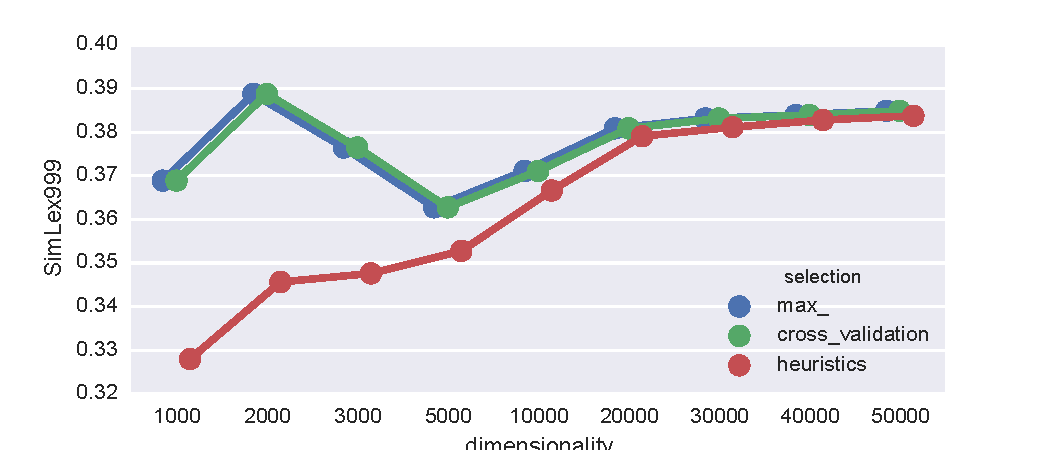
\includegraphics[width=0.5\textwidth]{supplement/figures/SimLex999-results}
  \caption{SimLex-999 results.}
  \label{fig:SimLex999-results}
\end{wrapfigure}

%%% Local Variables:
%%% mode: latex
%%% TeX-master: "../thesis"
%%% End:


\subsubsection{Max selection}
\label{sec:max-selection-simlex}

Figure~\ref{fig:SimLex999-results} illustrates the results based on the best model selection and Table~\ref{tab:parameters} shows the results together with picked parameters. Note that maximum selection is identical with cross-validation: they pick the same models.

In general model performance increases as the dimensionality increases. However, the best result of 0.389 is achieved with a 2000 dimensional space, this could be an example of overfitting. Model performance becomes changes for dimensions grater than 20000.

For spaces with dimensionality less than 5000 \texttt{freq} 1 and inner product yield best results. Otherwise, cosine with \logNSCPMI/, smoothing $\alpha=0.75$ and shifting $k=0.7$ gives the best results.

\begin{table}
  \centering

  \begin{tabular}{rrlllrl}
\toprule
 dimensionality &  SimLex999 &  freq &  discr &     cds &  neg &     similarity \\
\midrule
           1\,000 &      0.369 &     1 &   spmi &       1 &  0.2 &  inner\_product \\
           2\,000 &      0.389 &     1 &  scpmi &  global &  0.7 &  inner\_product \\
           3\,000 &      0.376 &     1 &   spmi &    0.75 &  0.2 &  inner\_product \\
           5\,000 &      0.363 &  logn &  scpmi &  global &  1.0 &            cos \\
          10\,000 &      0.371 &  logn &  scpmi &       1 &  0.7 &            cos \\
          20\,000 &      0.381 &  logn &  scpmi &    0.75 &  0.7 &            cos \\
          30\,000 &      0.383 &  logn &  scpmi &    0.75 &  0.7 &            cos \\
          40\,000 &      0.384 &  logn &  scpmi &    0.75 &  0.7 &            cos \\
          50\,000 &      0.385 &  logn &  scpmi &    0.75 &  0.7 &            cos \\
\bottomrule
\end{tabular}


  \caption{SimLex-999 Max selection.}
  \label{tab:Simlex999-max-selection}
\end{table}


\subsubsection{Heuristics}
\label{sec:heuristics-simlex}

\begin{wraptable}[8]{O}{0.5\textwidth}
  \vspace{-1em}
  \centering

  \begin{tabular}{lr}
\toprule
      parameter &  partial $R^2$ \\
\midrule
     similarity &       0.38 \\
           freq &       0.27 \\
            neg &       0.24 \\
 dimensionality &       0.08 \\
          discr &       0.08 \\
            cds &       0.06 \\
\bottomrule
\end{tabular}


  \caption{SimLex-999 feature ablation}
  \label{tab:SimLex999-ablation}
\end{wraptable}


% \begin{figure}

  \centering

  \begin{subfigure}[t]{0.49\textwidth}
    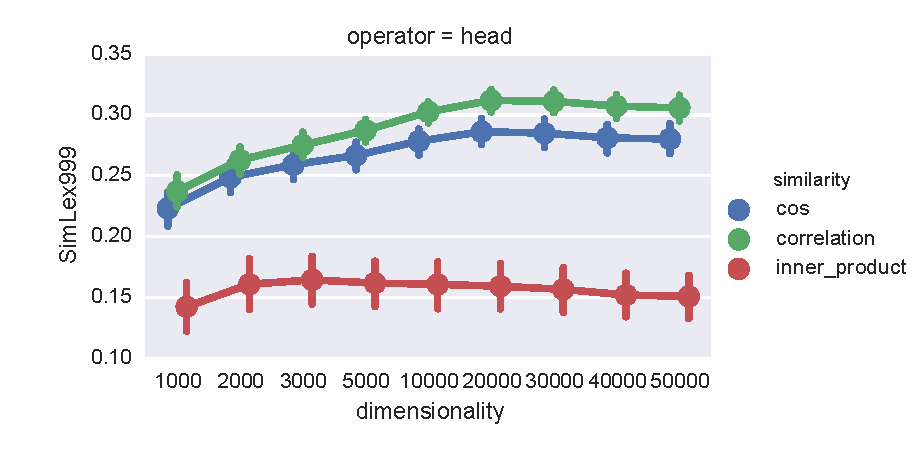
\includegraphics[width=\textwidth]{supplement/figures/SimLex999-interaction-similarity}
    \caption{similarity}
    \label{fig:SimLex999-interaction-similarity}
  \end{subfigure}
  \begin{subfigure}[t]{0.49\textwidth}
    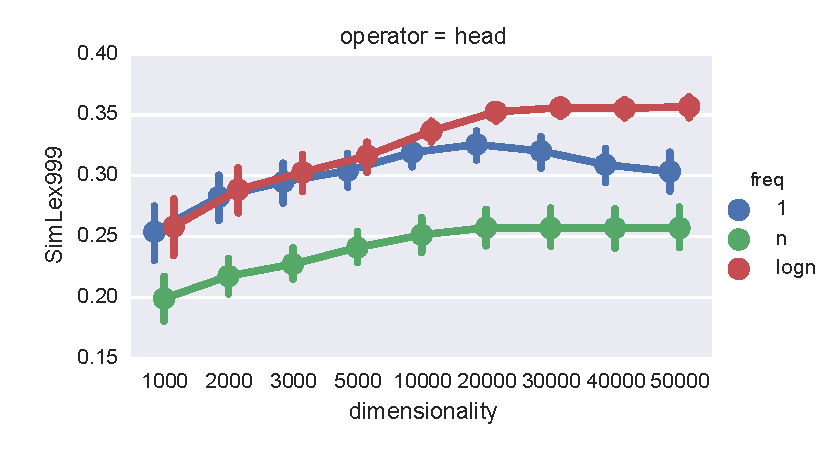
\includegraphics[width=\textwidth]{supplement/figures/SimLex999-interaction-freq}
    \caption{\texttt{freq}}
    \label{fig:SimLex999-interaction-freq}
  \end{subfigure}

  \begin{subfigure}[t]{0.49\textwidth}
    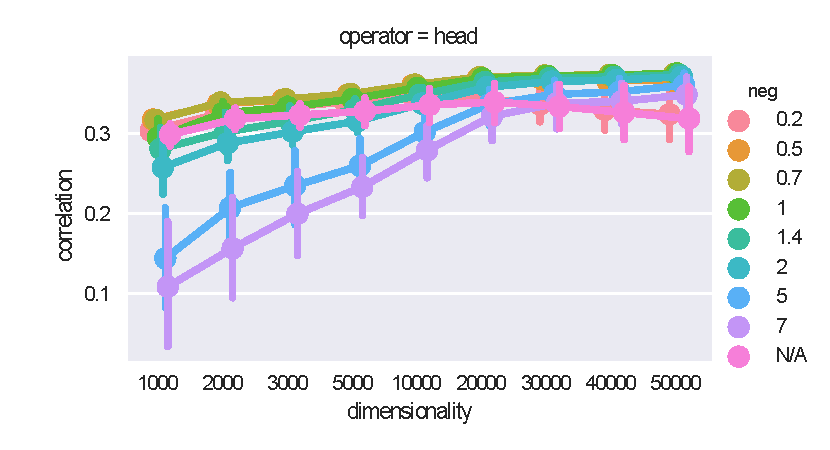
\includegraphics[width=\textwidth]{supplement/figures/SimLex999-interaction-neg}
    \caption{\texttt{neg}}
    \label{fig:SimLex999-interaction-neg}
  \end{subfigure}
  \begin{subfigure}[t]{0.49\textwidth}
    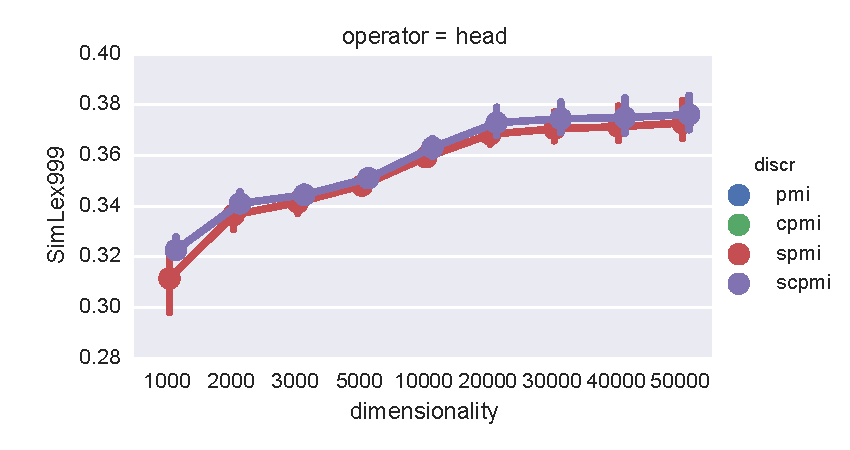
\includegraphics[width=\textwidth]{supplement/figures/SimLex999-interaction-discr}
    \caption{\texttt{discr}}
    \label{fig:SimLex999-interaction-discr}
  \end{subfigure}

  \begin{subfigure}[t]{0.49\textwidth}
    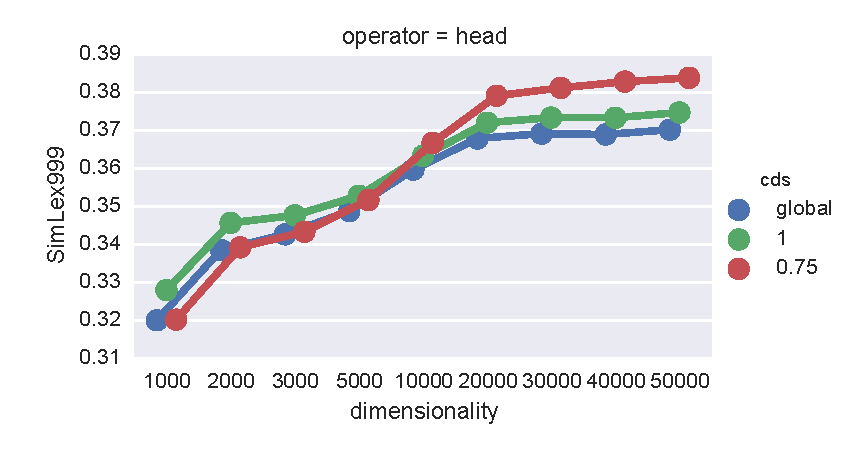
\includegraphics[width=\textwidth]{supplement/figures/SimLex999-interaction-cds}
    \caption{\texttt{cds}}
    \label{fig:SimLex999-interaction-cds}
  \end{subfigure}

  \caption{SimLex-999 parameter interaction. Parameters are shown in the order of their influence.}
  \label{fig:SimLex999-interaction}
\end{figure}

%%% Local Variables:
%%% mode: latex
%%% TeX-master: "../thesis"
%%% End:


The linear model achieves an adjusted $R^2$ of 0.867, indicating that the model is able to predict model performance based on parameter selection quite well. Table~\ref{tab:SimLex999-ablation} shows partial $R^2$ scores for parameters. The most influential parameters in decreasing order are similarity, \texttt{freq} and \texttt{neg}.

% \begin{wrapfigure}{O}{0.5\textwidth}
\begin{figure}
  % \vspace{-30pt}
  \centering

  \begin{subfigure}[t]{0.49\textwidth}
    \hspace{-20pt}
  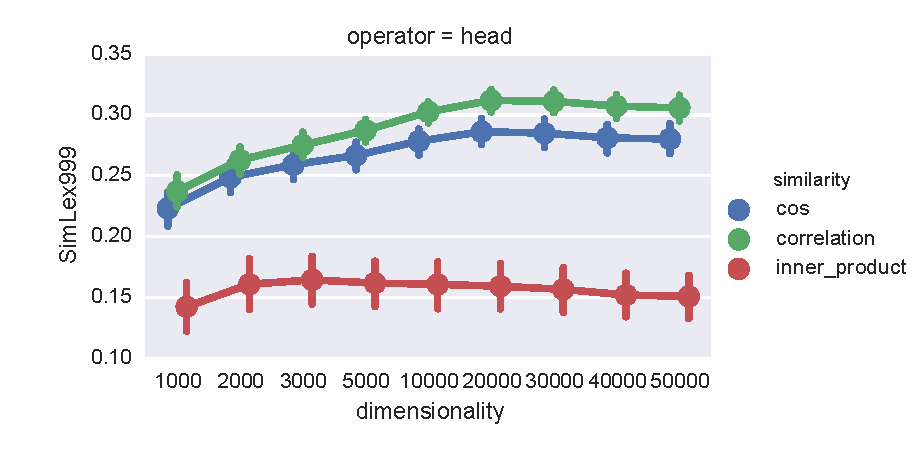
\includegraphics[width=1.1\textwidth]{supplement/figures/SimLex999-interaction-similarity}

  \caption{Similarity measure}
  \label{fig:SimLex999-similarity}

  \end{subfigure}
  \begin{subfigure}[t]{0.49\textwidth}

  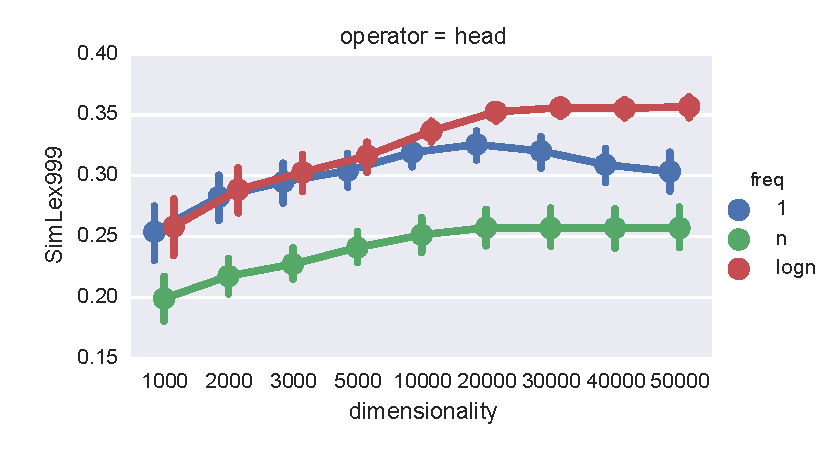
\includegraphics[width=\textwidth]{supplement/figures/SimLex999-interaction-freq}

  \caption{\texttt{freq}}
  \label{fig:SimLex999-freq}

  \end{subfigure}


  \begin{subfigure}[t]{0.49\textwidth}
  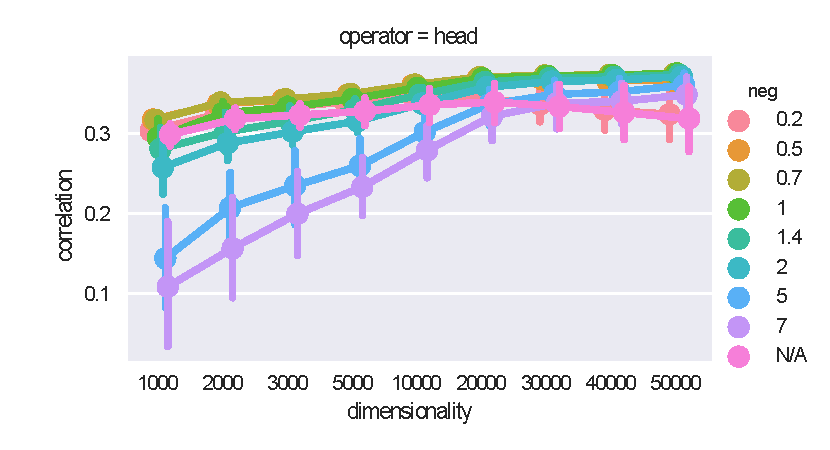
\includegraphics[width=\textwidth]{supplement/figures/SimLex999-interaction-neg}

  \caption{\texttt{neg}}
  \label{fig:SimLex999-neg}
  \end{subfigure}
  \begin{subfigure}[t]{0.49\textwidth}
  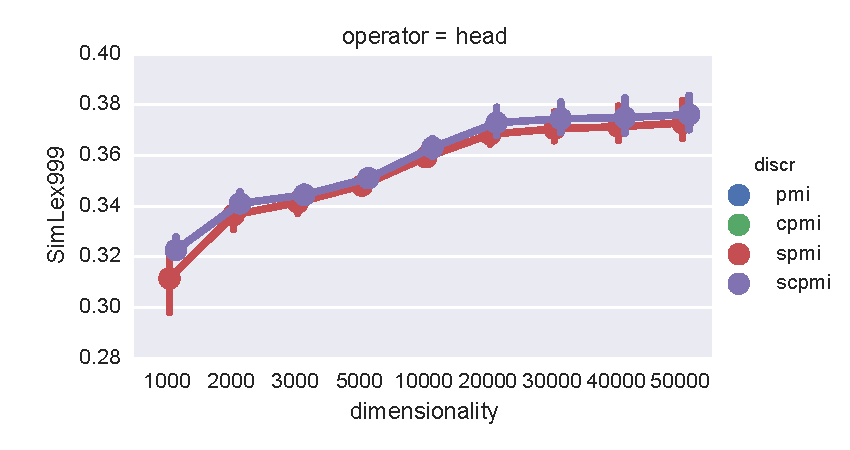
\includegraphics[width=\textwidth]{supplement/figures/SimLex999-interaction-discr}

  \caption{\texttt{discr}}
  \label{fig:SimLex999-discr}
  \end{subfigure}
  
  \caption[SimLex-999 influence of the similarity measure, \texttt{freq}, \texttt{neg} and \texttt{discr}]{SimLex-999 influence of the similarity measure, \texttt{freq}, \texttt{neg} and \texttt{discr}. Error bars indicate the 95\% confidence interval over the group of results.}
\end{figure}

Figure~\ref{fig:SimLex999-similarity} shows the average performance of similarity measures. Correlation outperforms all other measures for all dimensions and peaks at the dimensionality of 20000.

\begin{figure}[h]
% \begin{wrapfigure}{O}{0.5\textwidth}
  % \vspace{-30pt}
  \centering

  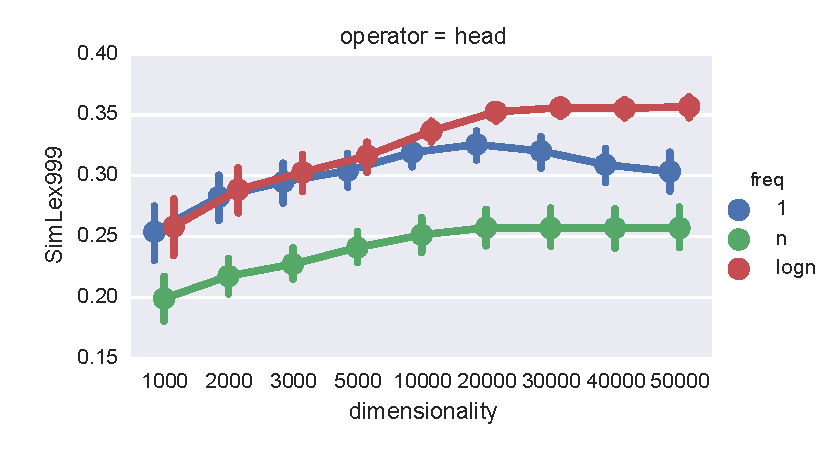
\includegraphics[width=0.5\textwidth]{supplement/figures/SimLex999-interaction-freq}

  \caption{SimLex-999 influence of \texttt{freq}.}
  \label{fig:SimLex999-freq}
\end{figure}

The influence of \texttt{freq}, the second parameter, is shown on Figure~\ref{fig:SimLex999-freq}. $\log n$ frequency outperforms other choices for all dimensions. After 20000 dimensions $\log n$'s performance stabilises.

\begin{figure}[b]
% \begin{wrapfigure}{O}{0.5\textwidth}
  % \vspace{-30pt}
  \centering

  \begin{subfigure}[t]{0.49\textwidth}
  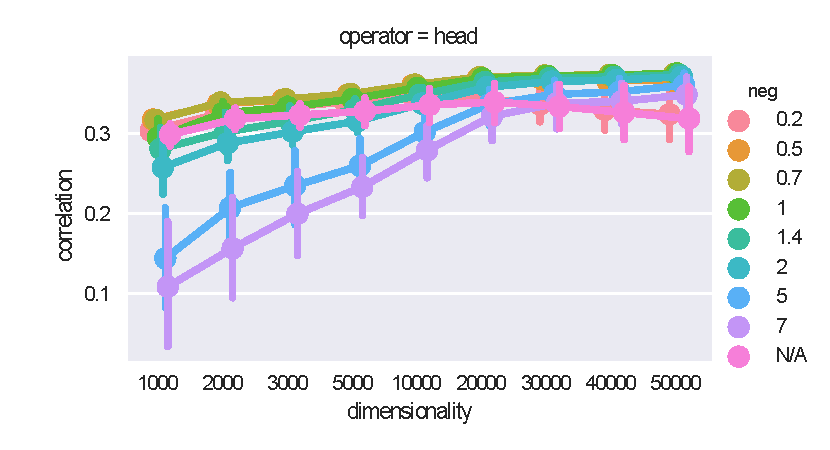
\includegraphics[width=\textwidth]{supplement/figures/SimLex999-interaction-neg}

  \caption{\texttt{neg}}
  \label{fig:SimLex999-neg}
  \end{subfigure}
  \begin{subfigure}[t]{0.49\textwidth}
  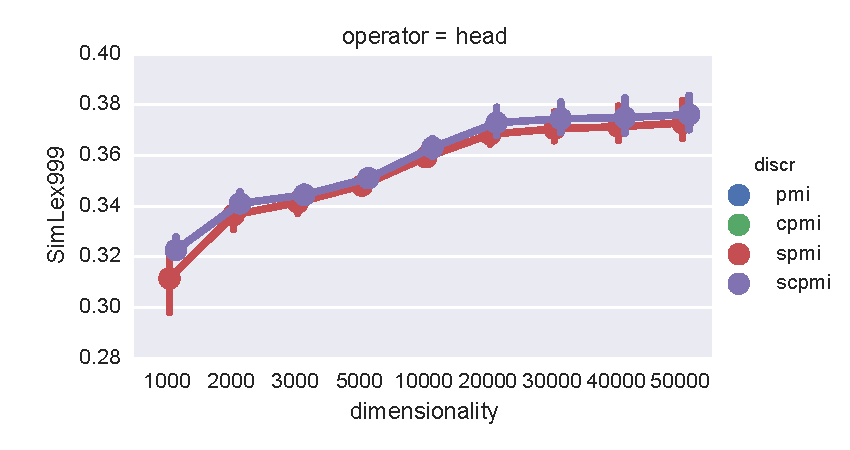
\includegraphics[width=\textwidth]{supplement/figures/SimLex999-interaction-discr}

  \caption{\texttt{discr}}
  \label{fig:SimLex999-discr}
  \end{subfigure}

  \caption{SimLex-999.}
\end{figure}

The third parameter \texttt{neg} of 0.7 shows the best performance (Figure~\ref{fig:SimLex999-neg}). However, there is little difference between models with dimensionality grater than 20000, apart from the models that do not perform shifting, whose performance peaks at 20000 dimensions.

\begin{figure}[h]
% \begin{wrapfigure}{O}{0.5\textwidth}
  % \vspace{-30pt}
  \centering

  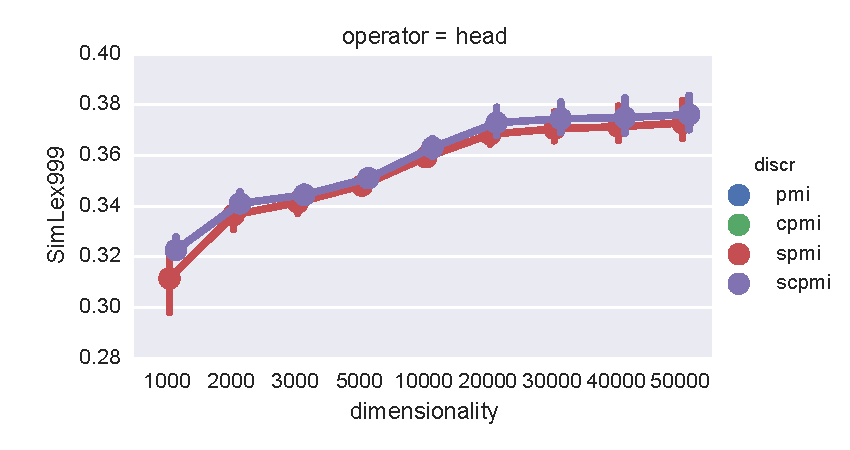
\includegraphics[width=0.5\textwidth]{supplement/figures/SimLex999-interaction-discr}

  \caption{SimLex-999 influence of \texttt{discr}. PMI and CPMI are not shown because at the step before models with shifting were chosen.}
  \label{fig:SimLex999-discr}
\end{figure}

There is little difference between SPMI and SCPMI performance with a little advantage to SCPMI (Figure~\ref{fig:SimLex999-discr}).

% \begin{figure}[h]
\begin{wrapfigure}[5]{O}{0.5\textwidth}
  \vspace{-30pt}
  \centering

  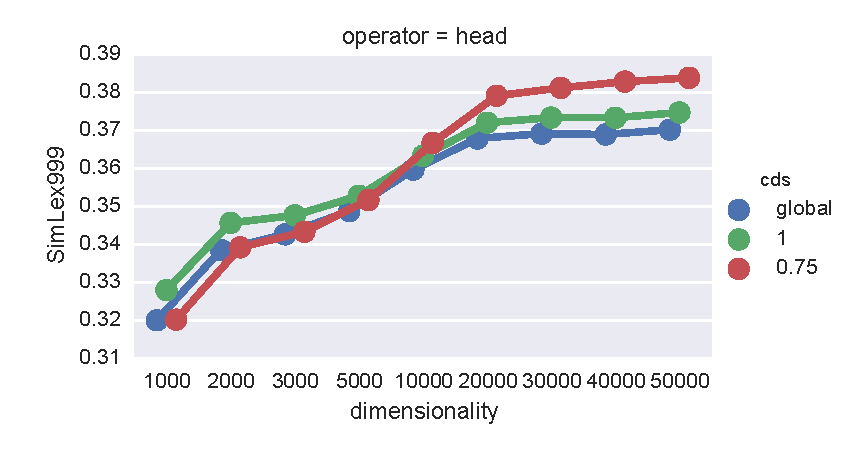
\includegraphics[width=0.5\textwidth]{supplement/figures/SimLex999-interaction-cds}
  \caption{SimLex-999 influence of \texttt{cds}.}
  \label{fig:SimLex999-cds}
\end{wrapfigure}

Finally, models benefit from context distribution smoothing, spaces with less than 10000 dimensions produce the best results with $\alpha = 1$, for spaces with higher dimensionality $\alpha = 0.75$ is the most advantageous (Figure~\ref{fig:SimLex999-cds}).

\todo[noline]{Contrast or compare results with \cite{milajevs:2016:SRW1}}

\paragraph{Difference with "Max" selection}

\begin{table}
  \centering

  \begin{tabular}{rrlllll}
\toprule
 dimensionality &  SimLex999 &  freq &  discr &   cds &  neg &   similarity \\
\midrule
           1\,000 &      0.328 &  logn &  scpmi &     1 &  0.7 &  correlation \\
           2\,000 &      0.346 &  logn &  scpmi &     1 &  0.7 &  correlation \\
           3\,000 &      0.348 &  logn &  scpmi &     1 &  0.7 &  correlation \\
           5\,000 &      0.353 &  logn &  scpmi &     1 &  0.7 &  correlation \\
          10\,000 &      0.367 &  logn &  scpmi &  0.75 &  0.7 &  correlation \\
          20\,000 &      0.379 &  logn &  scpmi &  0.75 &  0.7 &  correlation \\
          30\,000 &      0.381 &  logn &  scpmi &  0.75 &  0.7 &  correlation \\
          40\,000 &      0.383 &  logn &  scpmi &  0.75 &  0.7 &  correlation \\
          \textbf{50\,000} &      \textbf{0.384} &  \textbf{logn} &  \textbf{scpmi} &  \textbf{0.75} &  \textbf{0.7} &  \textbf{correlation} \\
\bottomrule
\end{tabular}


  \caption{SimLex-999 selection based on heuristics. The highest value is 0.384.
  The values that are grater than 0.361 are indistinguishable from the highest score.}
  \label{tab:Simlex999-heuristics-selection}
\end{table}


As expected manual parameter selection is more stable. Both selection models agree on parameters for highly dimensional spaces ($D \geq 2000$), with an exception of similarity: Max selection prefers cosine, while manual prefers correlation based similarity measure. Because of this, manual selection does not pick the best result of the 2000 dimensional model, but at the 50000 dimensions  a model selected manually scores 0.001 lower: 0.384 versus 0.385 as also seen on Figure~\ref{fig:SimLex999-results}.

The average relative difference between Max selection and heuristics is 0.039.

\subsection{MEN}
\label{sec:men}

\subsubsection{Max selection}
\label{sec:max-selection-men}

\begin{figure}
  \centering

    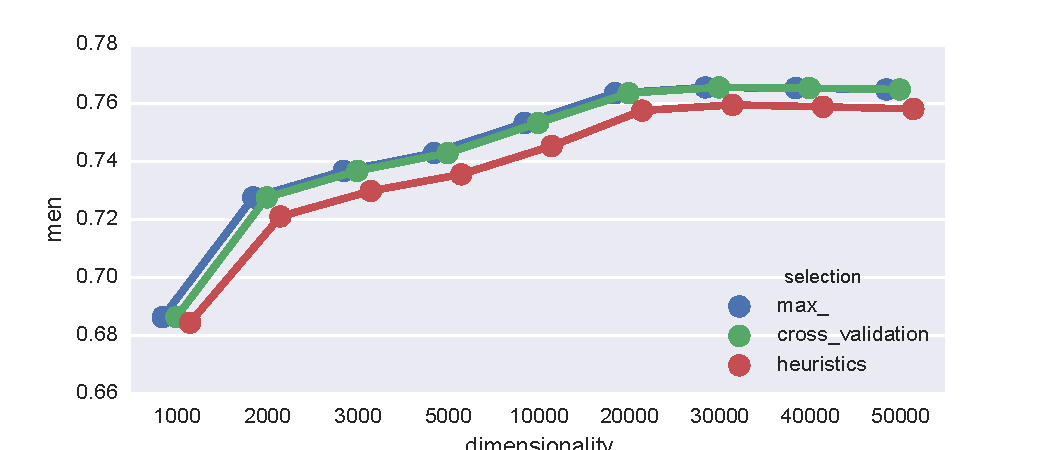
\includegraphics[width=0.5\textwidth]{supplement/figures/men-results}
  \caption{MEN results.}
  \label{fig:men-results}
\end{figure}

%%% Local Variables:
%%% mode: latex
%%% TeX-master: "../thesis"
%%% End:


Figure~\ref{fig:SimLex999-results} shows the selection results. Again, cross-validation results are identical with Max selection. Table~\ref{tab:men-max-selection} shows the results together with the selected models.

\begin{table}[b]
  \centering

  \begin{tabular}{rrlllrl}
\toprule
 dimensionality &    men &  freq &  discr &     cds &  neg &   similarity \\
\midrule
           1\,000 &  0.686 &     1 &  scpmi &  global &  1.4 &  correlation \\
           2\,000 &  0.728 &  logn &  scpmi &       1 &  0.7 &          cos \\
           3\,000 &  0.737 &  logn &  scpmi &       1 &  0.7 &          cos \\
           5\,000 &  0.743 &  logn &  scpmi &    0.75 &  0.7 &          cos \\
          10\,000 &  0.753 &  logn &  scpmi &    0.75 &  1.0 &  correlation \\
          20\,000 &  0.763 &  logn &  scpmi &    0.75 &  1.0 &  correlation \\
          \textbf{30\,000} &  \textbf{0.765} &  \textbf{logn} &  \textbf{scpmi} &    \textbf{0.75} &  \textbf{1.0} &  \textbf{correlation} \\
          \textbf{40\,000} &  \textbf{0.765} &  \textbf{logn} &  \textbf{scpmi} &    \textbf{0.75} &  \textbf{1.0} &  \textbf{correlation} \\
          \textbf{50\,000} &  \textbf{0.765} &  \textbf{logn} &  \textbf{scpmi} &    \textbf{0.75} &  \textbf{1.0} &  \textbf{correlation} \\
\bottomrule
\end{tabular}


  \caption{MEN Max selection}
  \label{tab:men-max-selection}
\end{table}


\subsubsection{Heuristics}
\label{sec:heuristics-men}


\subsection{Universal parameter selection for lexical datasets}
\label{sec:Universal-lexical-param-selection}

% SimLex --> Men
% Men --> SimLex
% Universal, normalized!

% Idea: find common parameters and take average over one for which there is not agreement. Normalize the result and repeat the heuristics selection?

\section{Similarity of sentences}
\label{sec:sentential}

\subsection{KS14}
\label{sec:ks14}


% \clearpage
% \KOMAoptions{paper=A3}
% % \addtolength{\textwidth}{1.35\textwidth}
% \recalctypearea

\newgeometry{margin=1.5cm}

\begin{landscape}
\thispagestyle{empty} %% Remove header and footer.

\begin{figure}
  \centering

  \begin{subfigure}[t]{0.49\textwidth}
    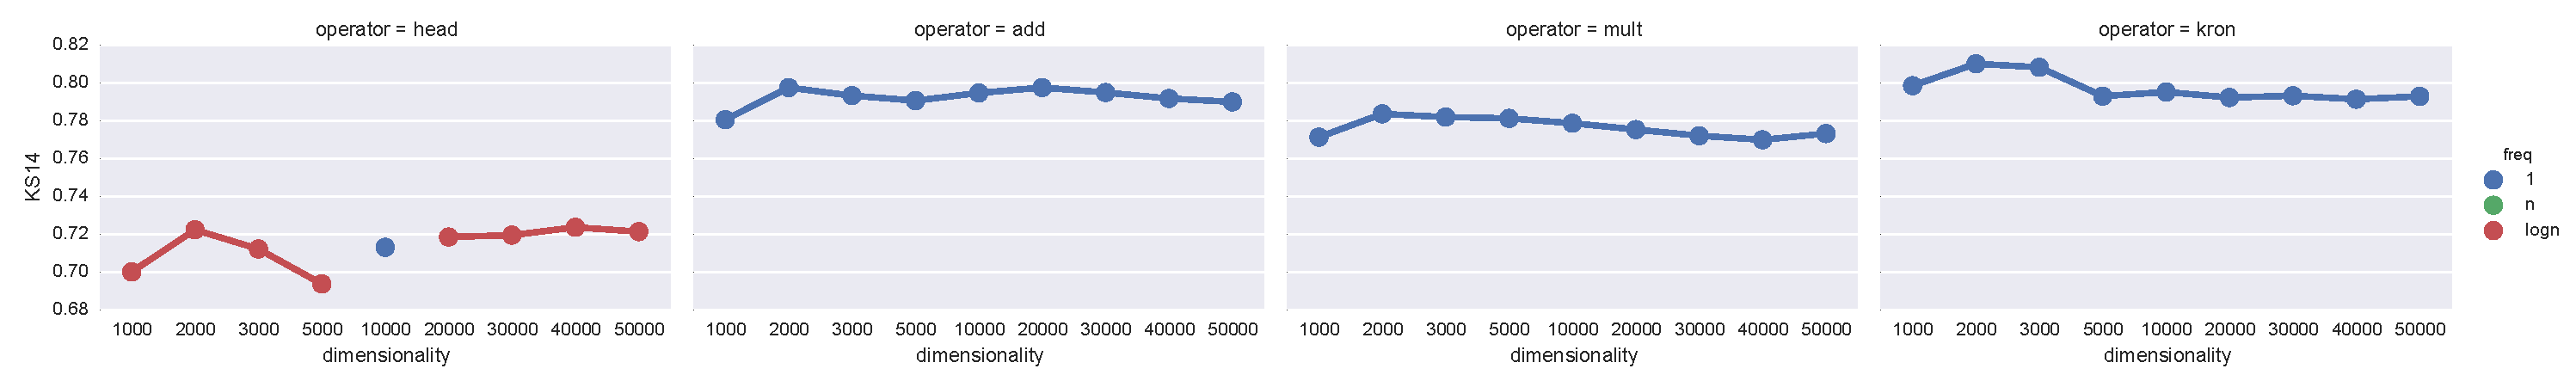
\includegraphics[width=\textwidth]{supplement/figures/KS14-max_-selection-freq}
    \caption{Max. Freq.}
    \label{fig:}
  \end{subfigure}
  \begin{subfigure}[t]{0.49\textwidth}
    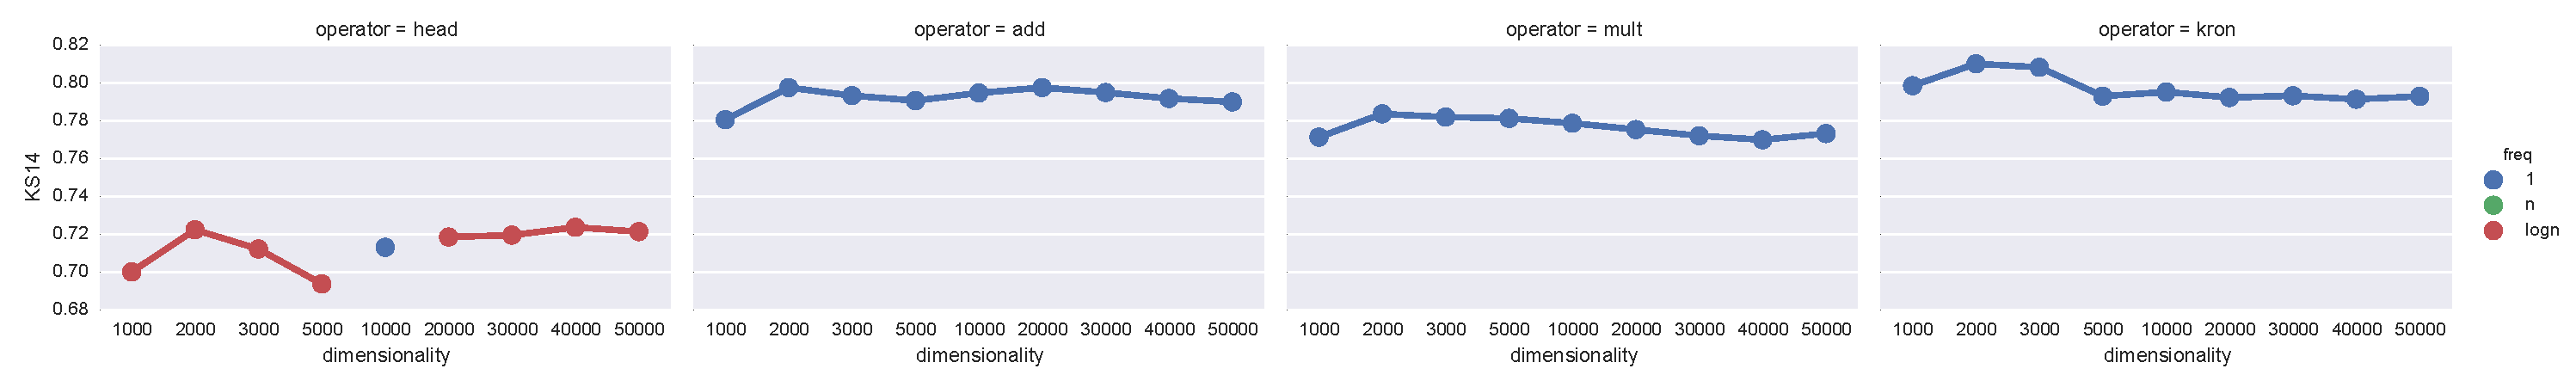
\includegraphics[width=\textwidth]{supplement/figures/KS14-cross_validation-selection-freq}
    \caption{CV. Freq.}
    \label{fig:}
  \end{subfigure}
  \begin{subfigure}[t]{0.49\textwidth}
    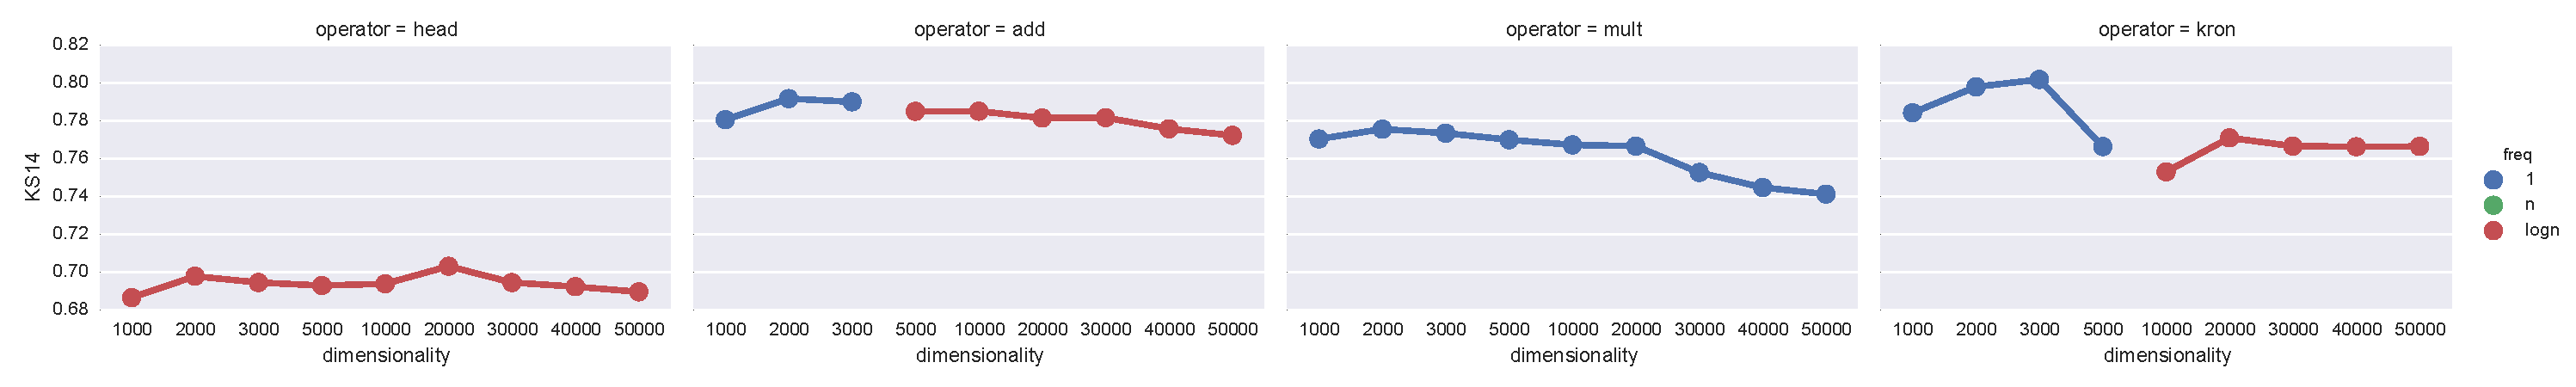
\includegraphics[width=\textwidth]{supplement/figures/KS14-heuristics-selection-freq}
    \caption{H. Freq.}
    \label{fig:}
  \end{subfigure}

  \begin{subfigure}[t]{0.49\textwidth}
    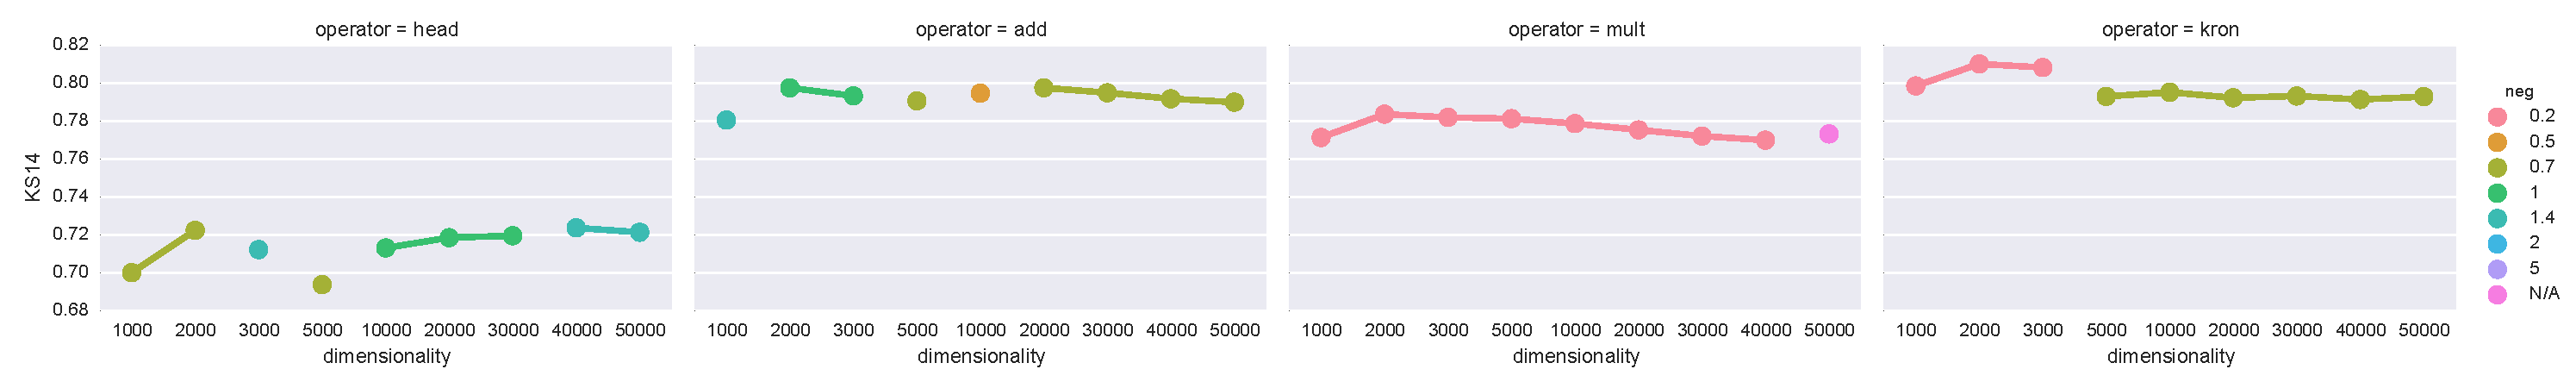
\includegraphics[width=\textwidth]{supplement/figures/KS14-max_-selection-neg}
    \caption{Max. Neg.}
    \label{fig:}
  \end{subfigure}
  \begin{subfigure}[t]{0.49\textwidth}
    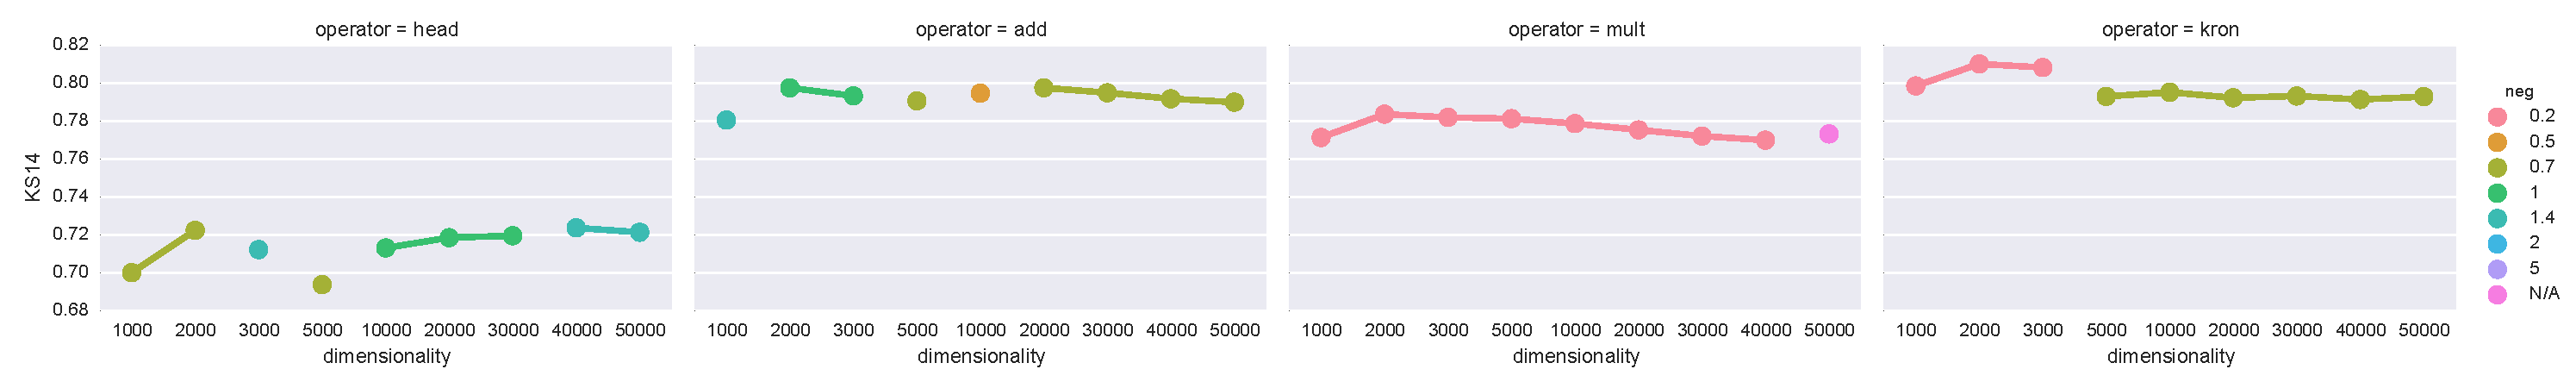
\includegraphics[width=\textwidth]{supplement/figures/KS14-cross_validation-selection-neg}
    \caption{CV. Neg.}
    \label{fig:}
  \end{subfigure}
  \begin{subfigure}[t]{0.49\textwidth}
    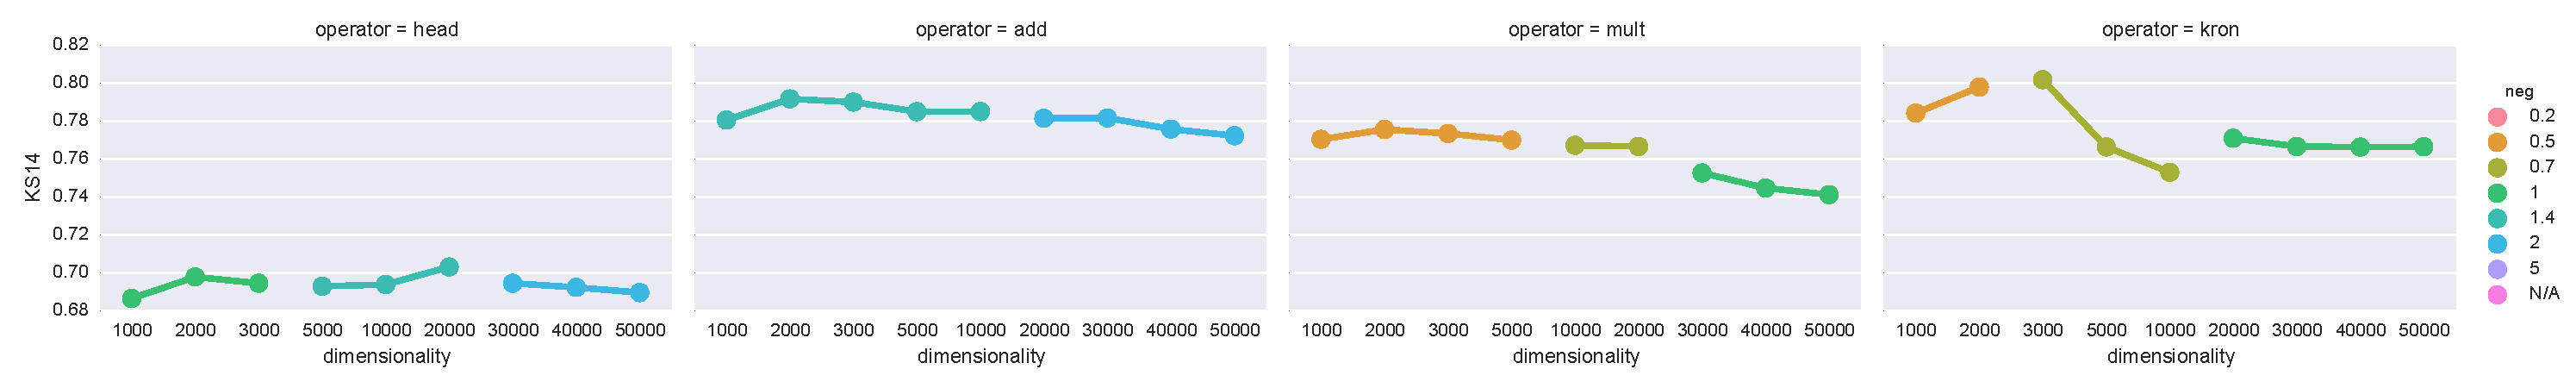
\includegraphics[width=\textwidth]{supplement/figures/KS14-heuristics-selection-neg}
    \caption{H. Neg.}
    \label{fig:}
  \end{subfigure}

  \begin{subfigure}[t]{0.49\textwidth}
    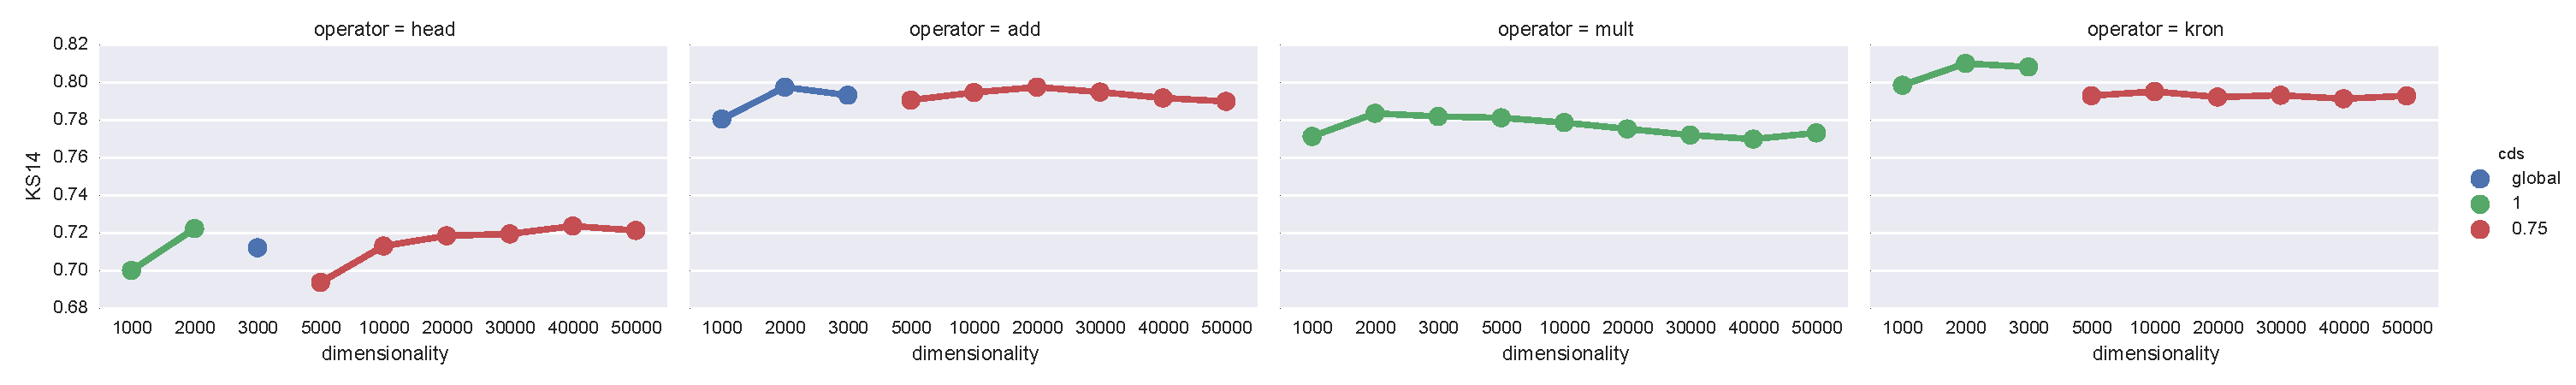
\includegraphics[width=\textwidth]{supplement/figures/KS14-max_-selection-cds}
    \caption{Max. CDS.}
    \label{fig:}
  \end{subfigure}
  \begin{subfigure}[t]{0.49\textwidth}
    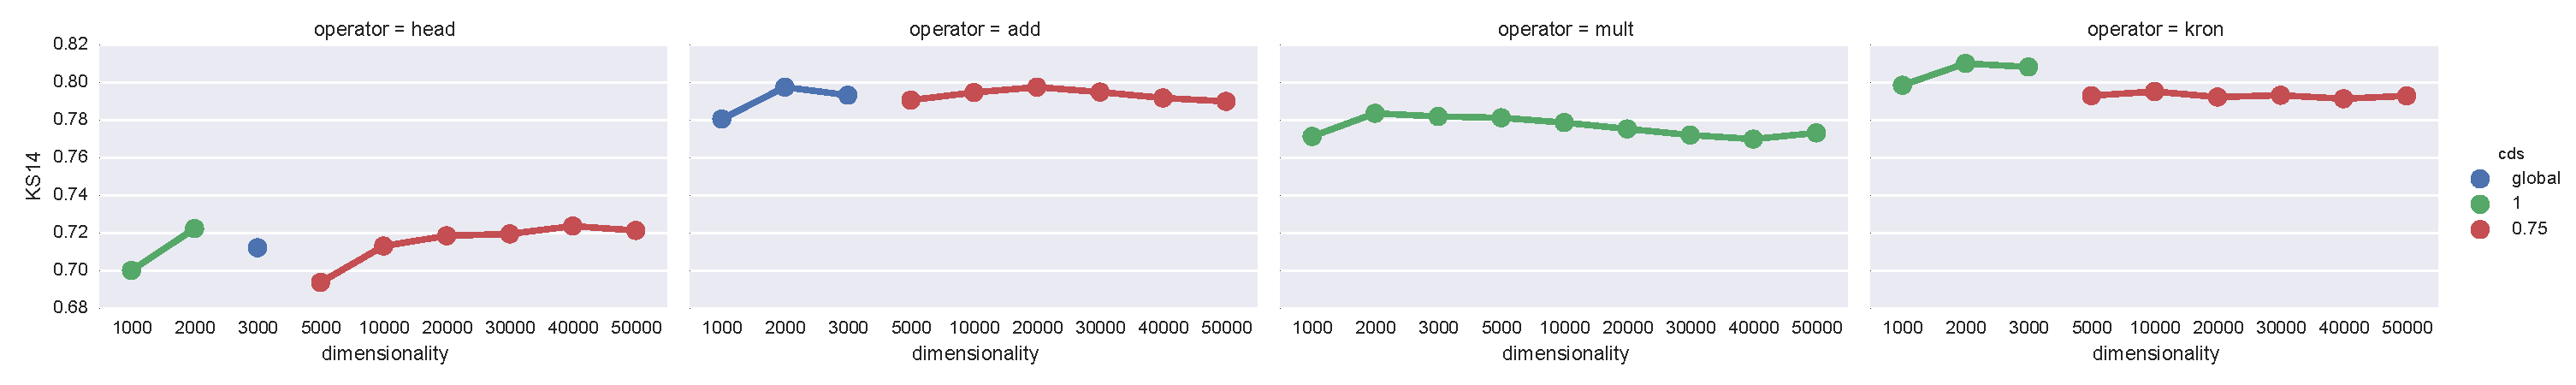
\includegraphics[width=\textwidth]{supplement/figures/KS14-cross_validation-selection-cds}
    \caption{CV. CDS.}
    \label{fig:}
  \end{subfigure}
  \begin{subfigure}[t]{0.49\textwidth}
    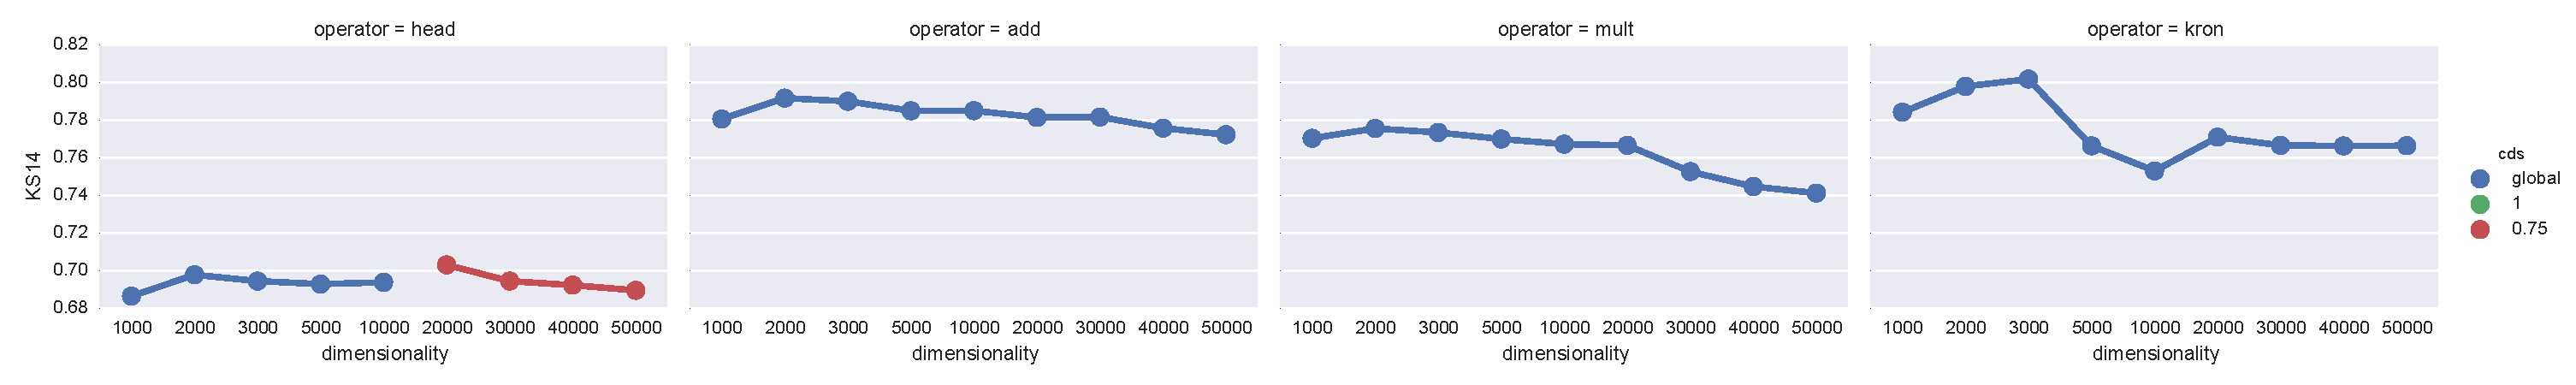
\includegraphics[width=\textwidth]{supplement/figures/KS14-heuristics-selection-cds}
    \caption{H. CDS.}
    \label{fig:}
  \end{subfigure}

  \begin{subfigure}[t]{0.49\textwidth}
    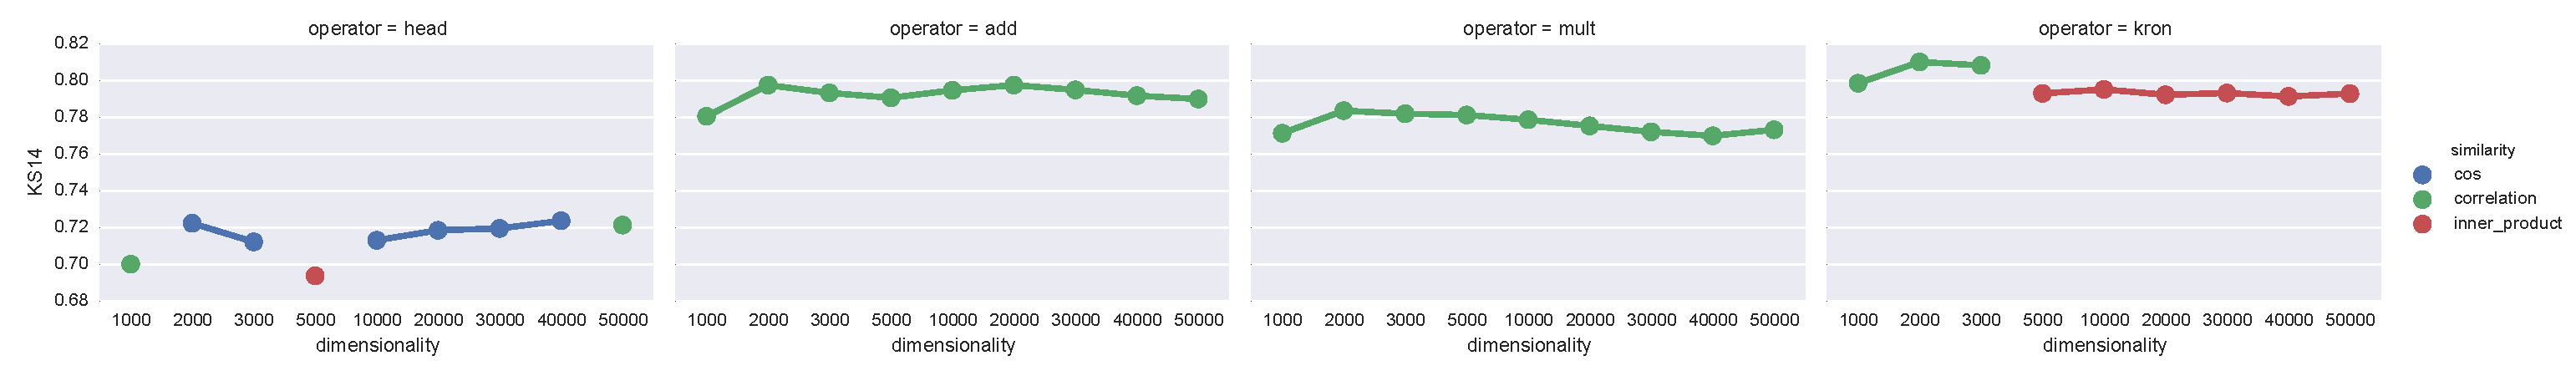
\includegraphics[width=\textwidth]{supplement/figures/KS14-max_-selection-similarity}
    \caption{Max. Sim.}
    \label{fig:}
  \end{subfigure}
  \begin{subfigure}[t]{0.49\textwidth}
    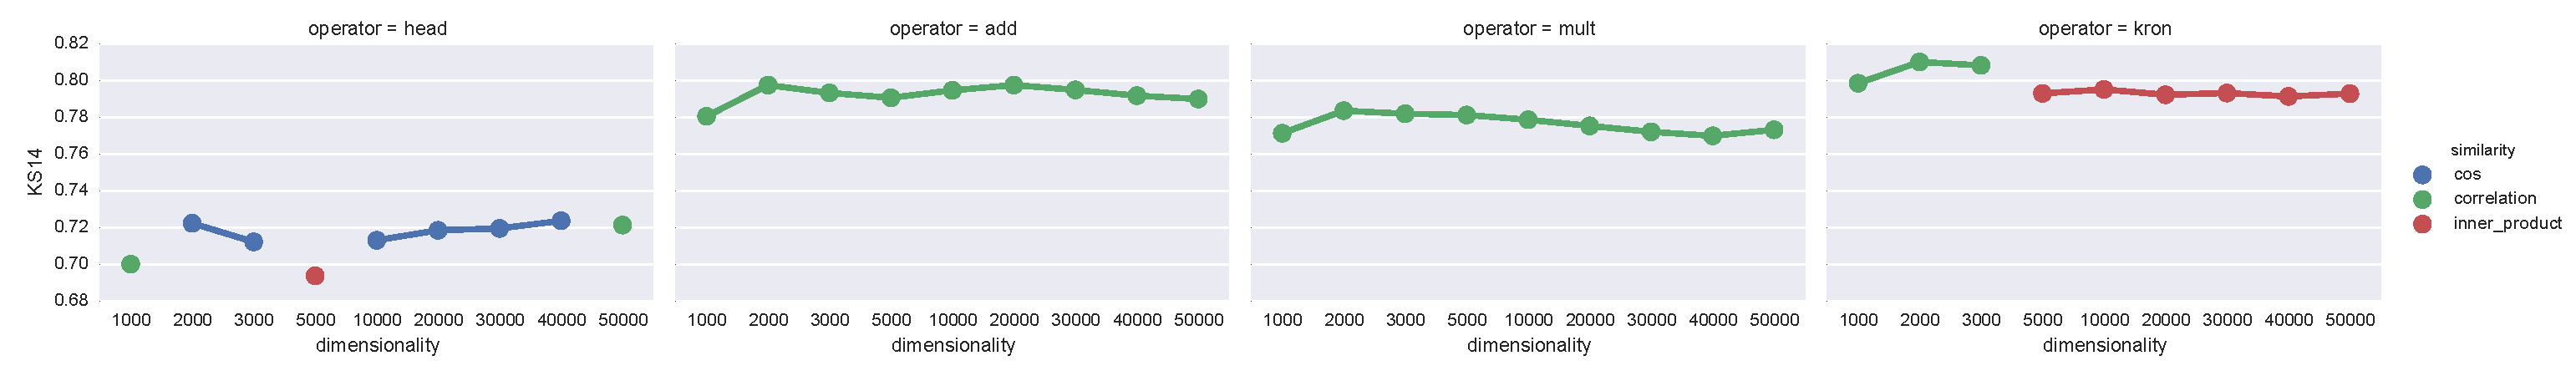
\includegraphics[width=\textwidth]{supplement/figures/KS14-cross_validation-selection-similarity}
    \caption{CV. Sim.}
    \label{fig:}
  \end{subfigure}
  \begin{subfigure}[t]{0.49\textwidth}
    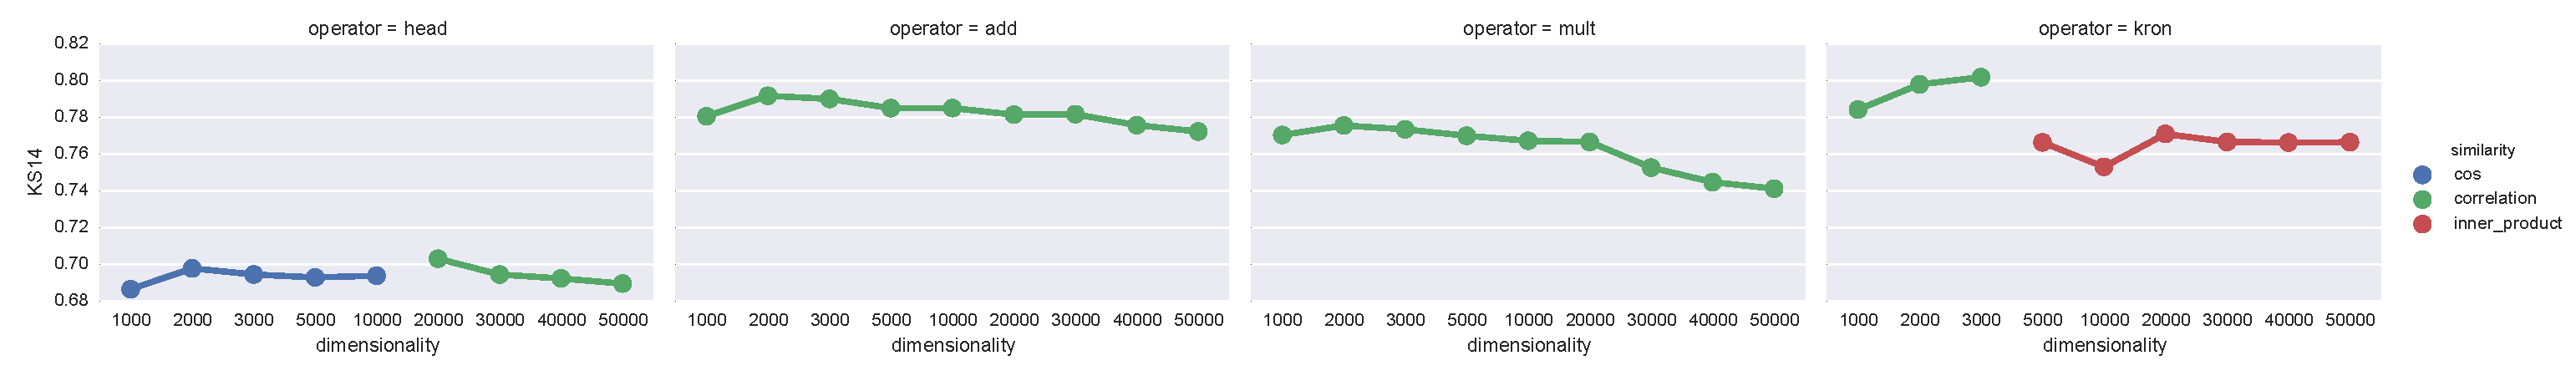
\includegraphics[width=\textwidth]{supplement/figures/KS14-heuristics-selection-similarity}
    \caption{H. Sim.}
    \label{fig:}
  \end{subfigure}

  \begin{subfigure}[t]{0.49\textwidth}
    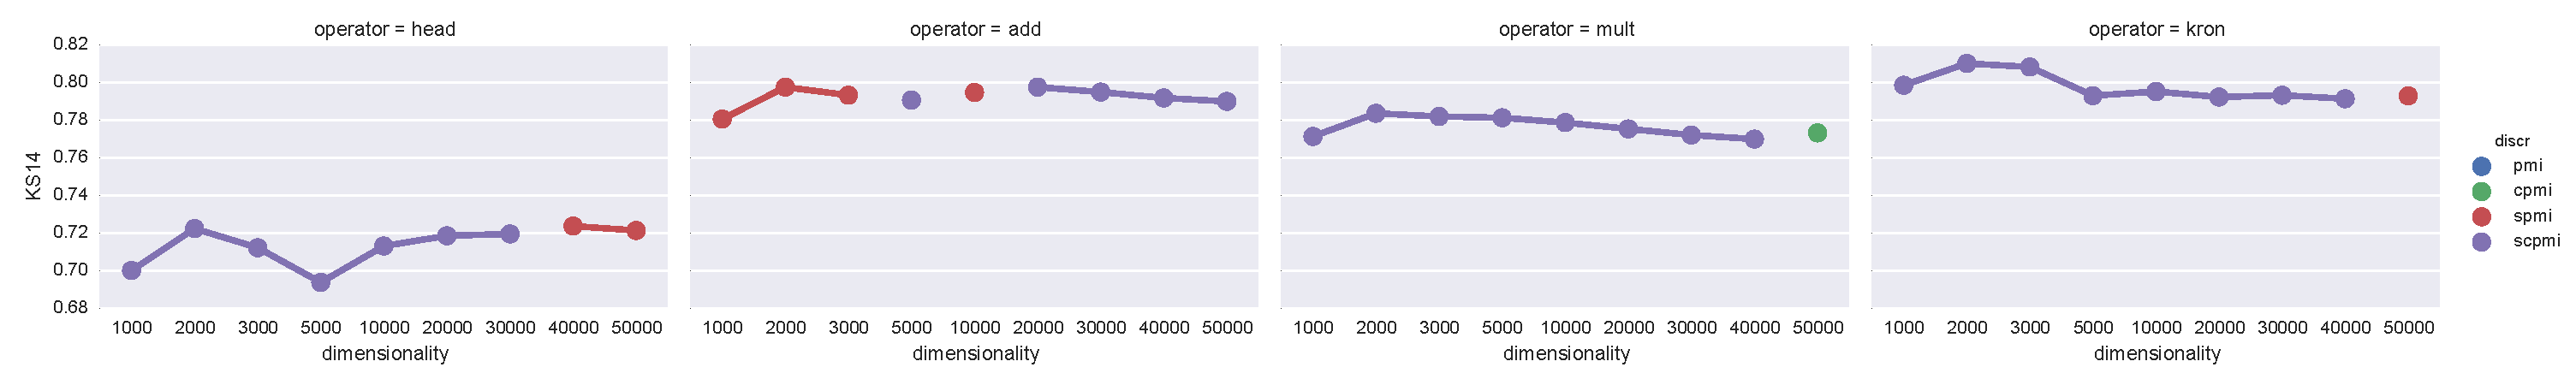
\includegraphics[width=\textwidth]{supplement/figures/KS14-max_-selection-discr}
    \caption{Max. Discr.}
    \label{fig:}
  \end{subfigure}
  \begin{subfigure}[t]{0.49\textwidth}
    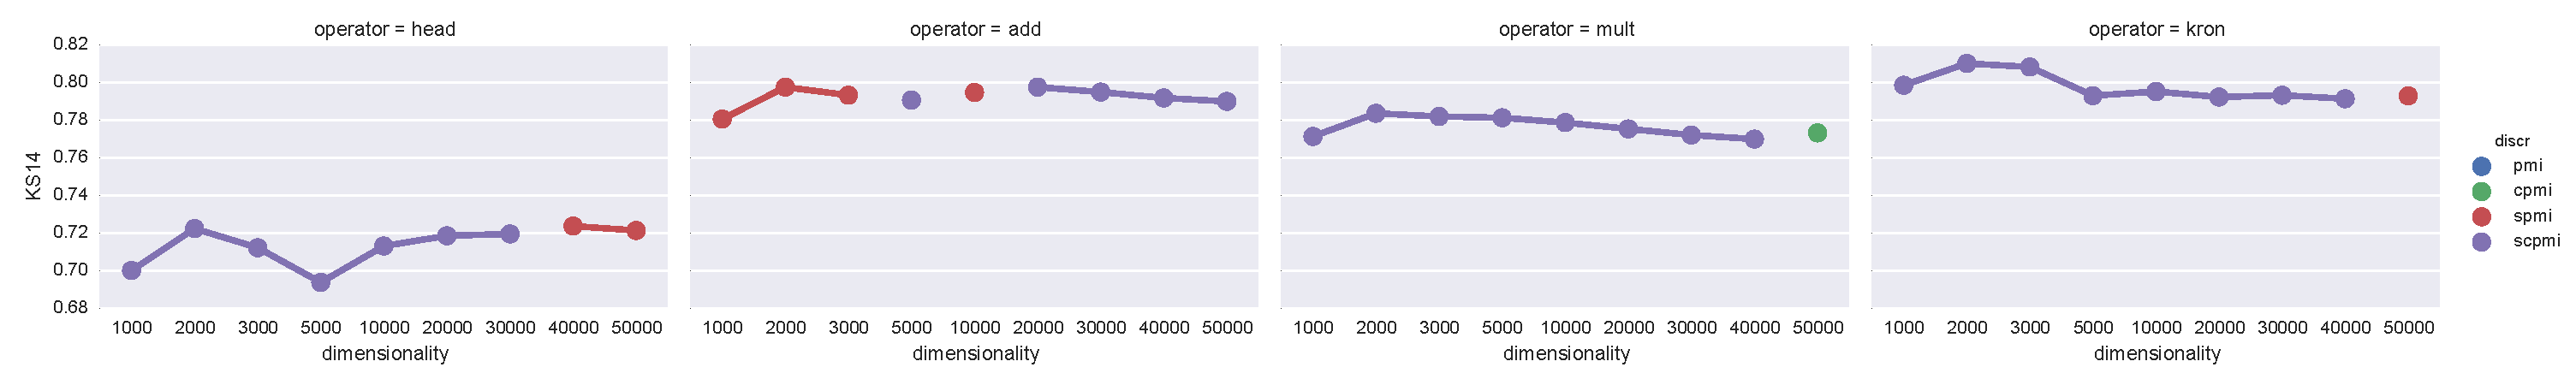
\includegraphics[width=\textwidth]{supplement/figures/KS14-cross_validation-selection-discr}
    \caption{CV. Discr.}
    \label{fig:}
  \end{subfigure}
  \begin{subfigure}[t]{0.49\textwidth}
    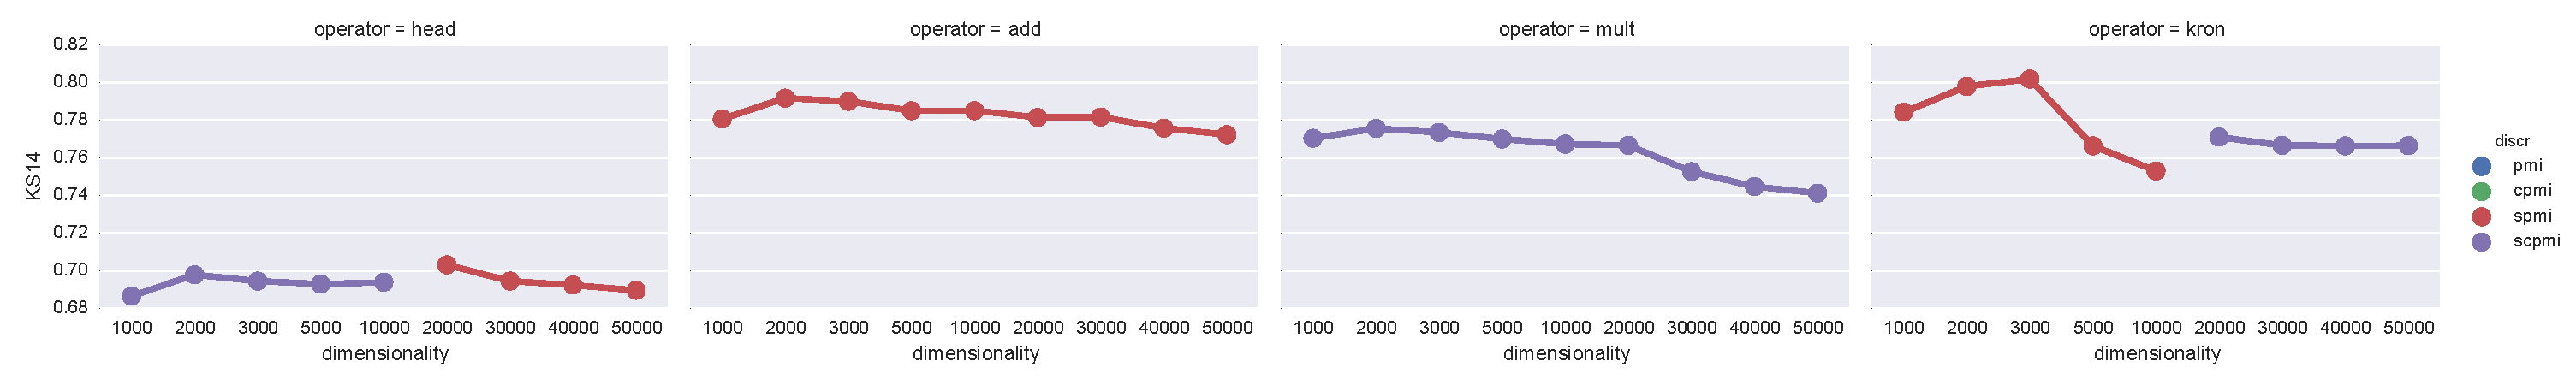
\includegraphics[width=\textwidth]{supplement/figures/KS14-heuristics-selection-discr}
    \caption{H. Discr.}
    \label{fig:}
  \end{subfigure}


  \caption{KS14 selection.}
  \label{fig:selection_ks14}
\end{figure}

\end{landscape}

\restoregeometry

% \clearpage
% \KOMAoptions{paper=A4,pagesize}
% \recalctypearea


\subsection{GS11}
\label{sec:gs11}

% \clearpage
% \KOMAoptions{paper=A3}
% % \addtolength{\textwidth}{1.35\textwidth}
% \recalctypearea

\newgeometry{margin=1.5cm}

\begin{landscape}
% \thispagestyle{empty} %% Remove header and footer.

\begin{figure}
  \centering

  \begin{subfigure}[t]{0.7\textwidth}
    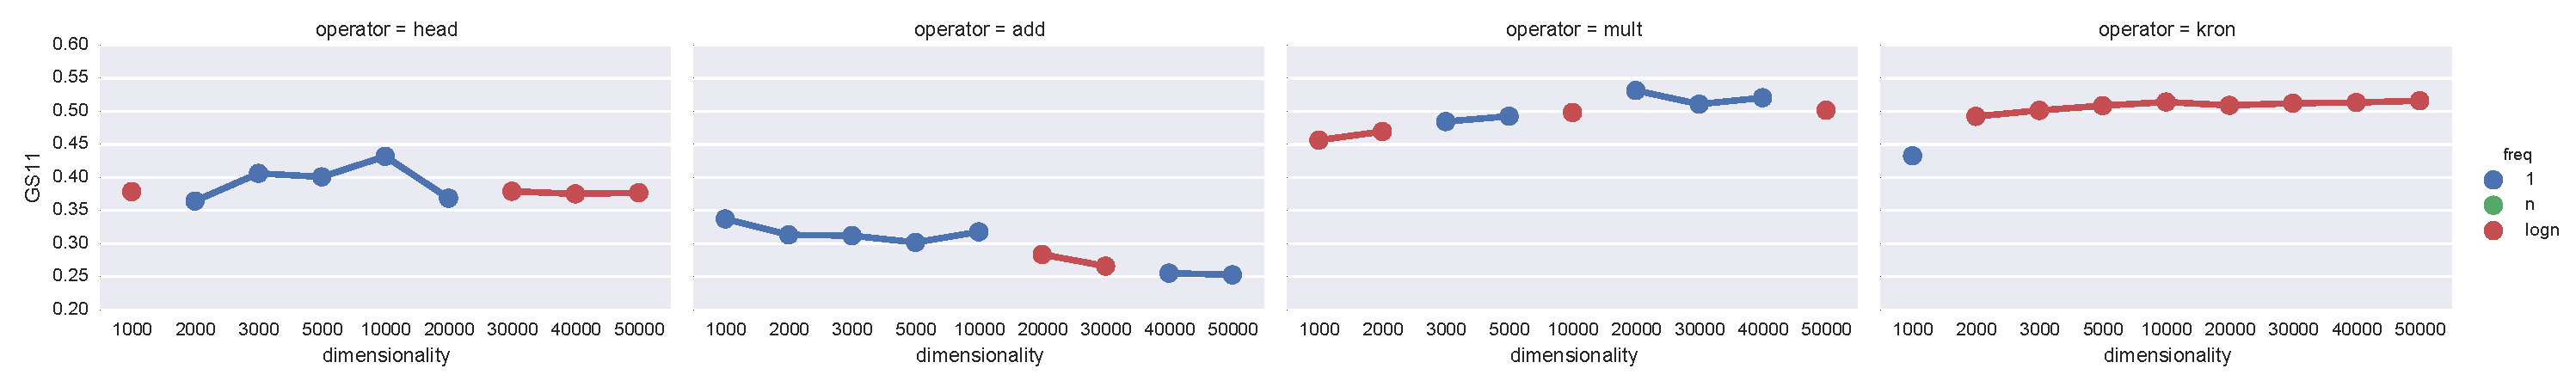
\includegraphics[width=\textwidth]{supplement/figures/GS11-max_-selection-freq}
    \caption{Max. Freq.}
    \label{fig:}
  \end{subfigure}
  % \begin{subfigure}[t]{0.7\textwidth}
  %   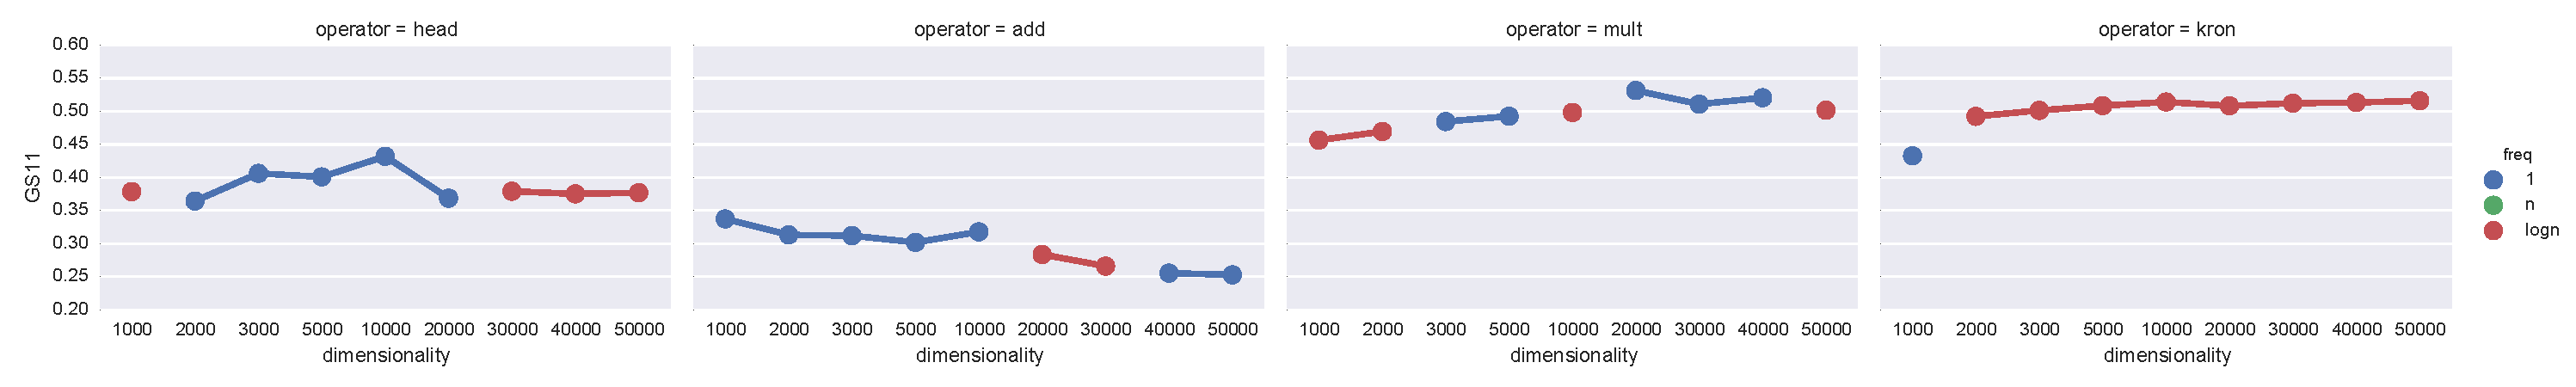
\includegraphics[width=\textwidth]{supplement/figures/GS11-cross_validation-selection-freq}
  %   \caption{CV. Freq.}
  %   \label{fig:}
  % \end{subfigure}
  \begin{subfigure}[t]{0.7\textwidth}
    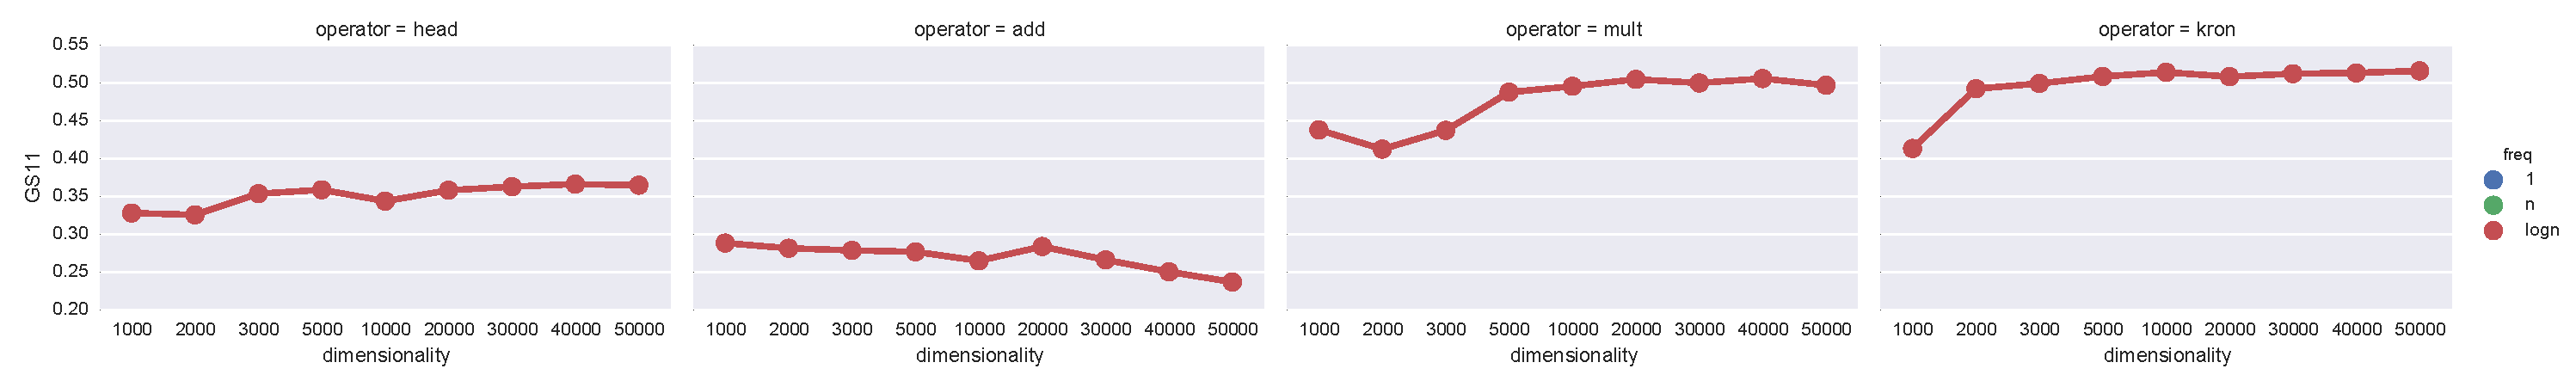
\includegraphics[width=\textwidth]{supplement/figures/GS11-heuristics-selection-freq}
    \caption{H. Freq.}
    \label{fig:}
  \end{subfigure}

  \begin{subfigure}[t]{0.7\textwidth}
    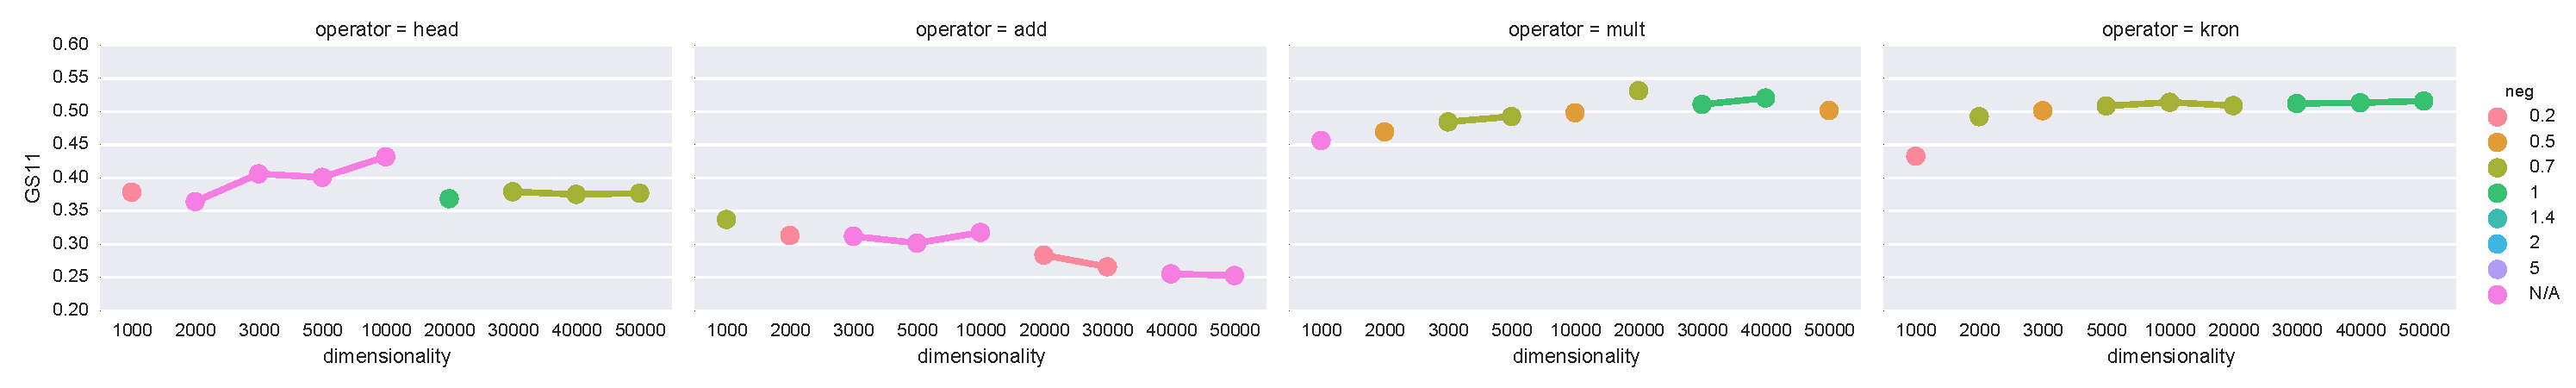
\includegraphics[width=\textwidth]{supplement/figures/GS11-max_-selection-neg}
    \caption{Max. Neg.}
    \label{fig:}
  \end{subfigure}
  % \begin{subfigure}[t]{0.7\textwidth}
  %   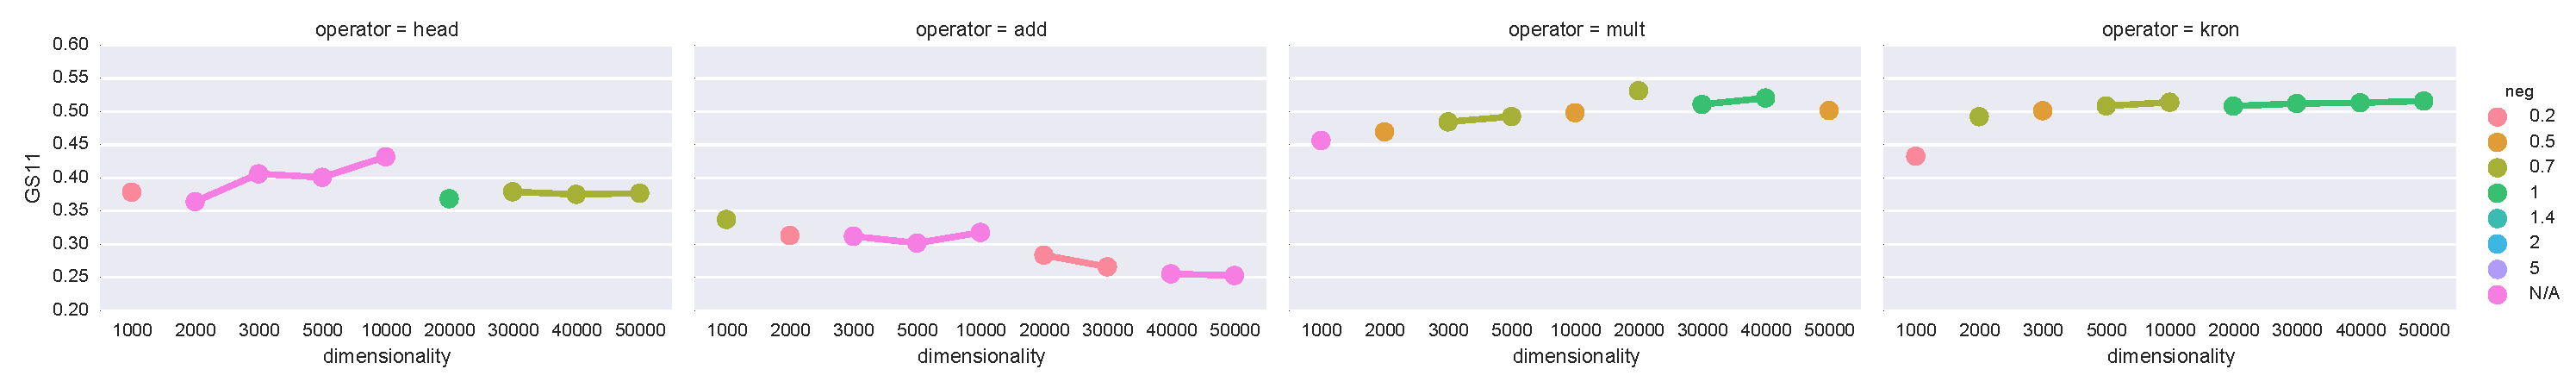
\includegraphics[width=\textwidth]{supplement/figures/GS11-cross_validation-selection-neg}
  %   \caption{CV. Neg.}
  %   \label{fig:}
  % \end{subfigure}
  \begin{subfigure}[t]{0.7\textwidth}
    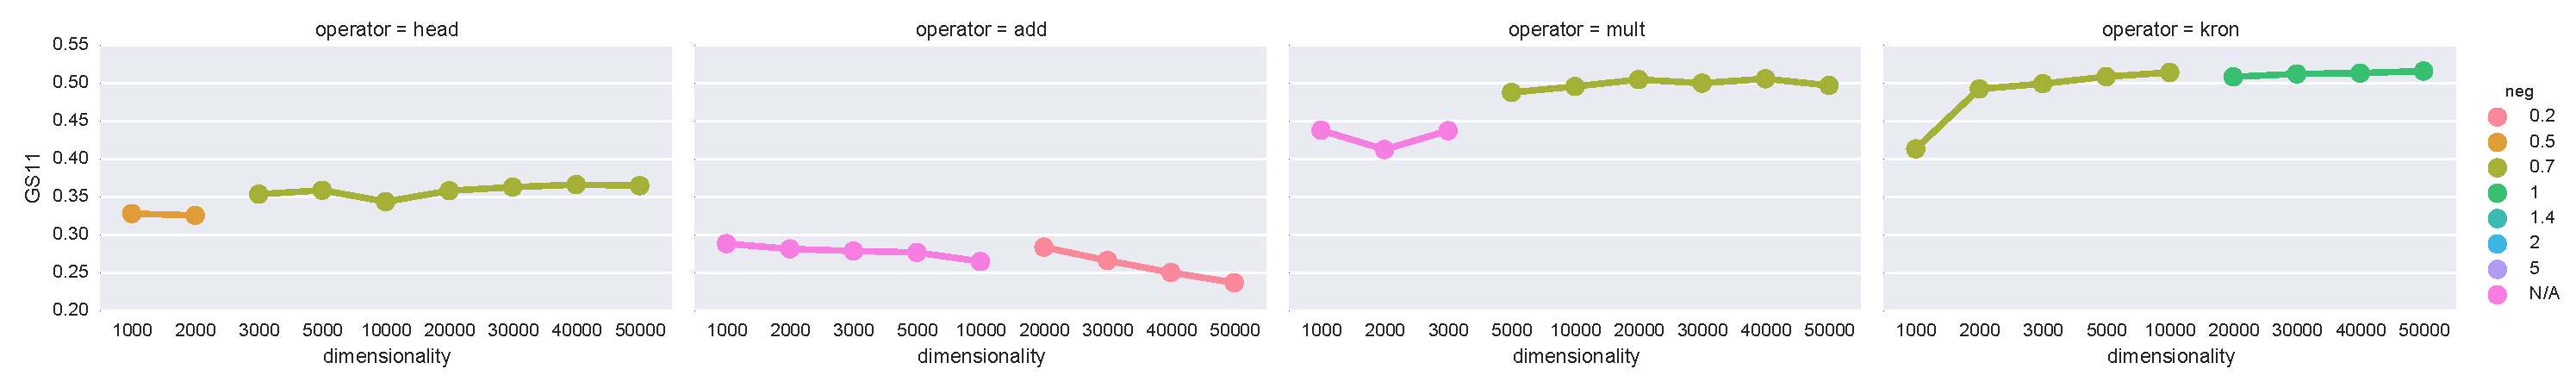
\includegraphics[width=\textwidth]{supplement/figures/GS11-heuristics-selection-neg}
    \caption{H. Neg.}
    \label{fig:}
  \end{subfigure}

  \begin{subfigure}[t]{0.7\textwidth}
    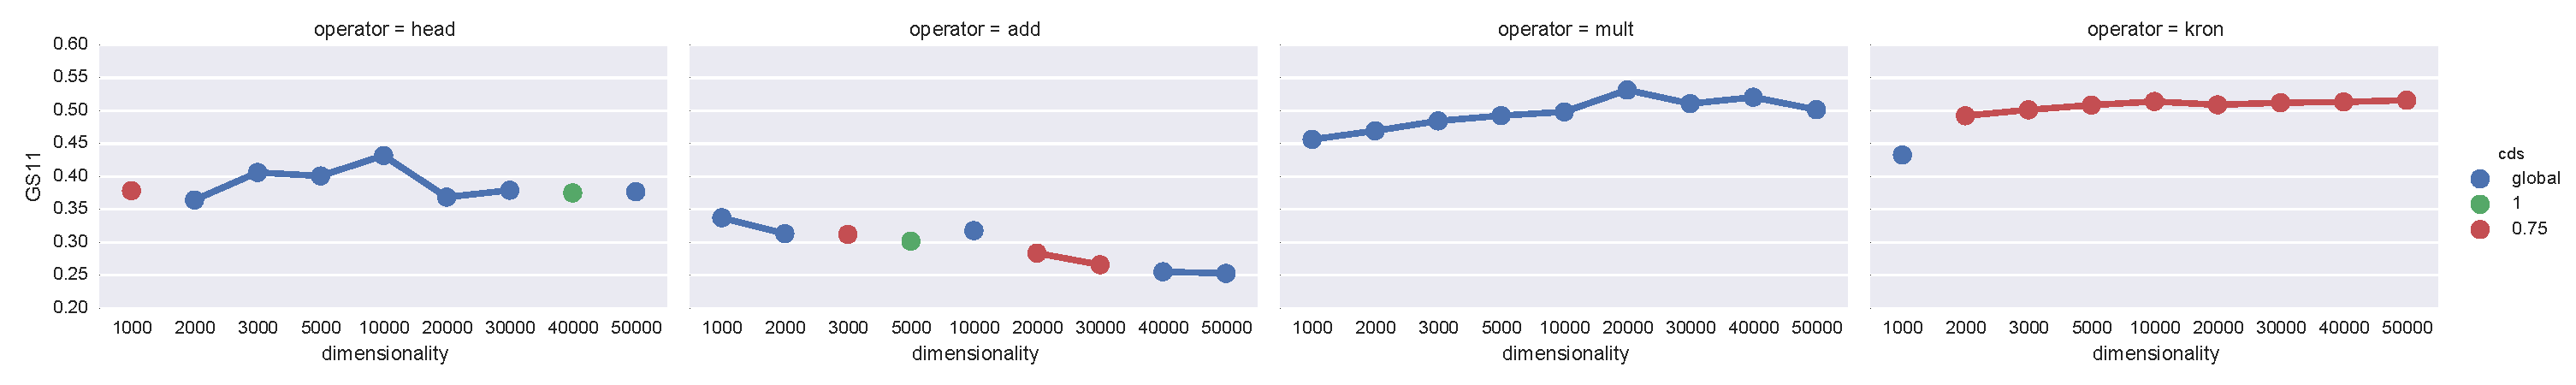
\includegraphics[width=\textwidth]{supplement/figures/GS11-max_-selection-cds}
    \caption{Max. CDS.}
    \label{fig:}
  \end{subfigure}
  % \begin{subfigure}[t]{0.7\textwidth}
  %   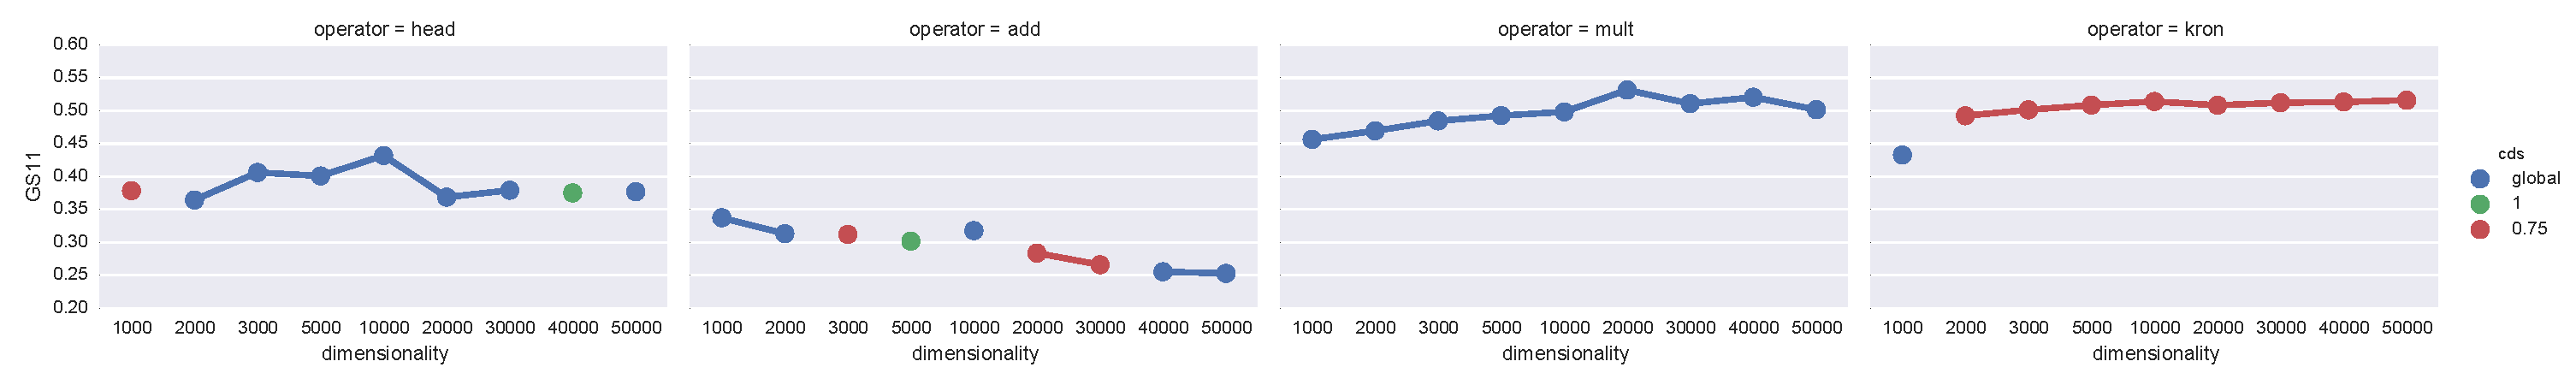
\includegraphics[width=\textwidth]{supplement/figures/GS11-cross_validation-selection-cds}
  %   \caption{CV. CDS.}
  %   \label{fig:}
  % \end{subfigure}
  \begin{subfigure}[t]{0.7\textwidth}
    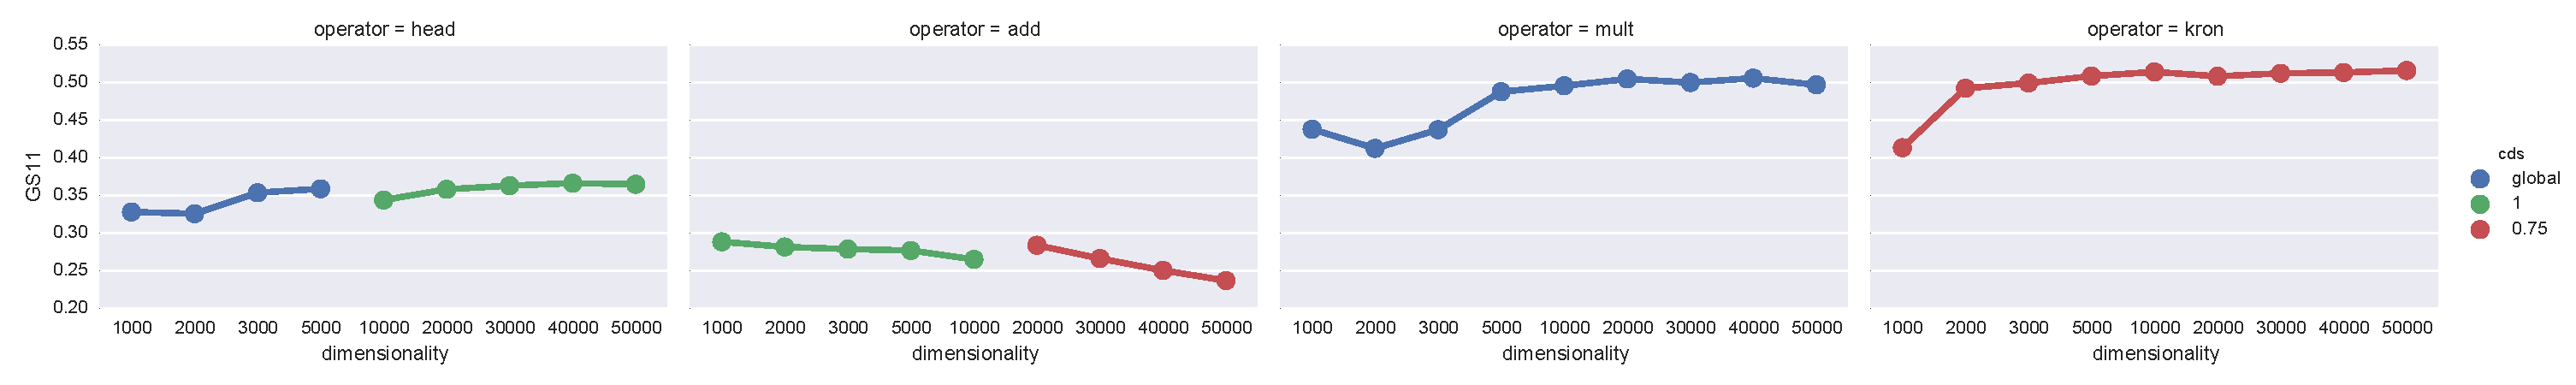
\includegraphics[width=\textwidth]{supplement/figures/GS11-heuristics-selection-cds}
    \caption{H. CDS.}
    \label{fig:}
  \end{subfigure}

  \begin{subfigure}[t]{0.7\textwidth}
    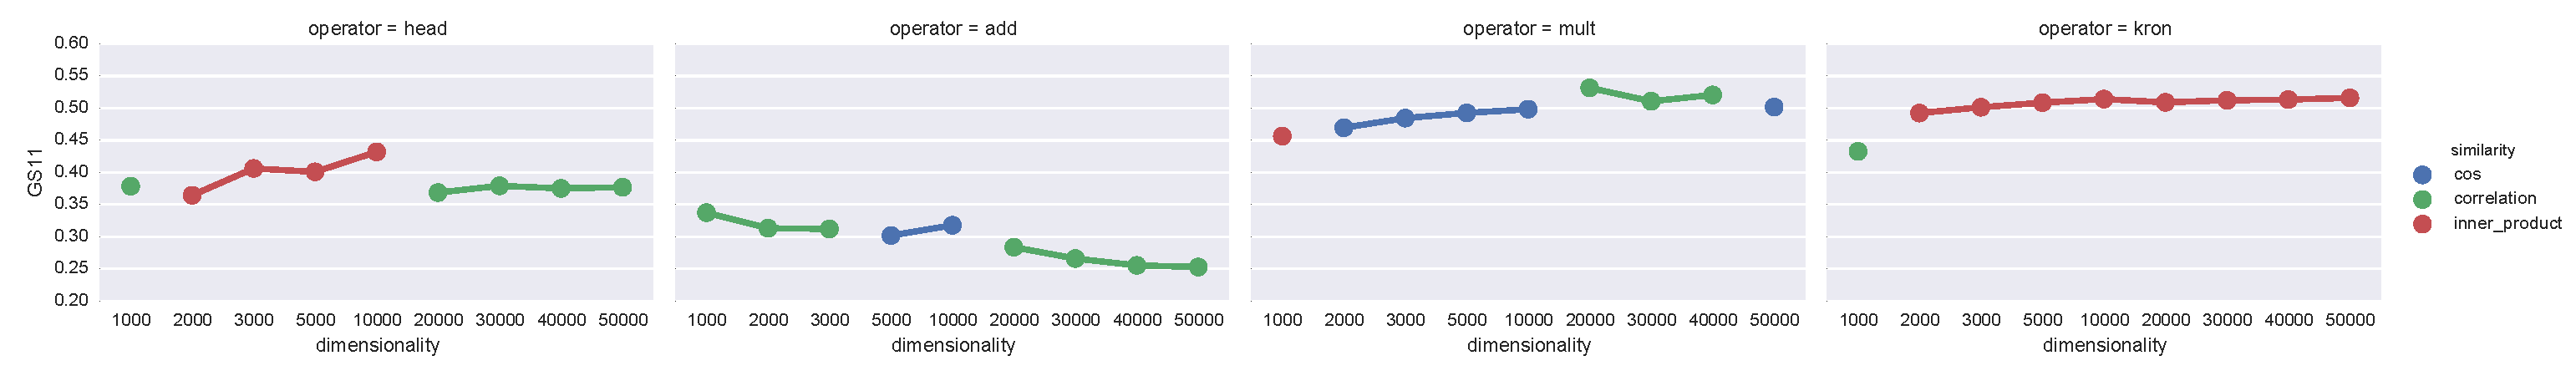
\includegraphics[width=\textwidth]{supplement/figures/GS11-max_-selection-similarity}
    \caption{Max. Sim.}
    \label{fig:}
  \end{subfigure}
  % \begin{subfigure}[t]{0.7\textwidth}
  %   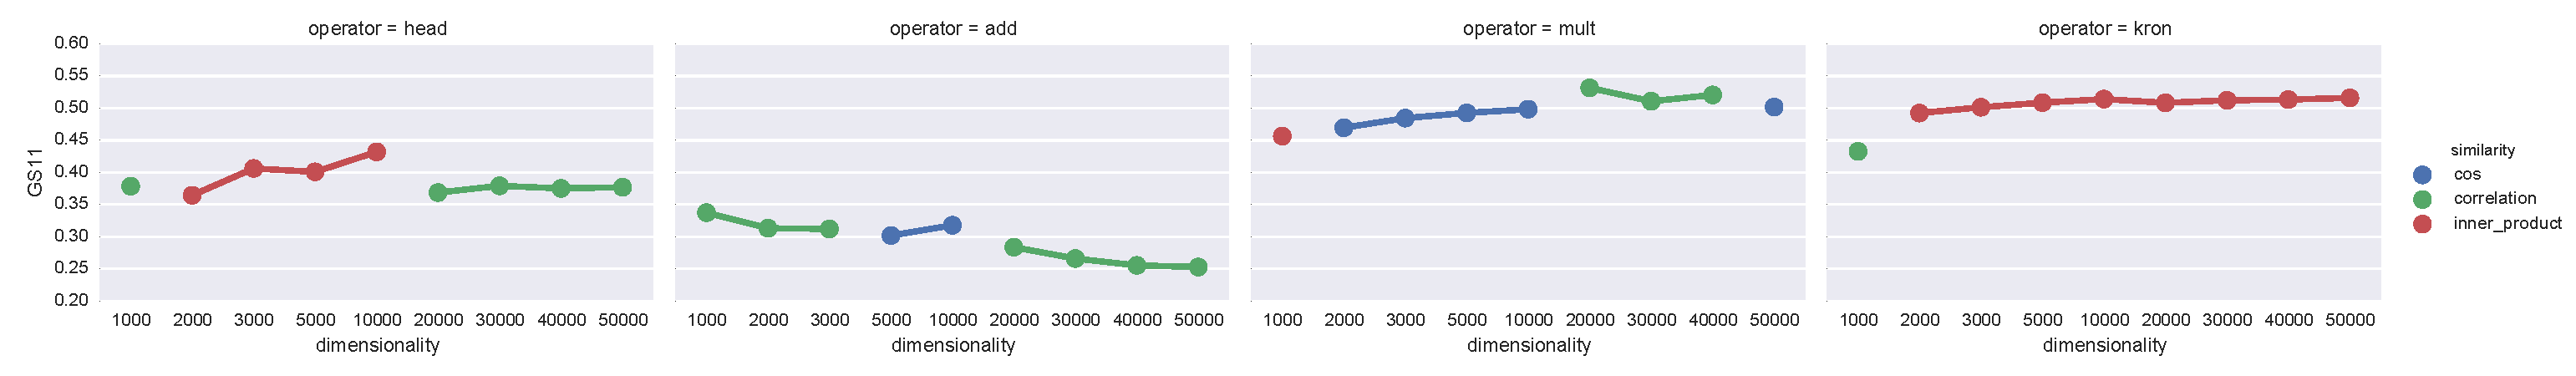
\includegraphics[width=\textwidth]{supplement/figures/GS11-cross_validation-selection-similarity}
  %   \caption{CV. Sim.}
  %   \label{fig:}
  % \end{subfigure}
  \begin{subfigure}[t]{0.7\textwidth}
    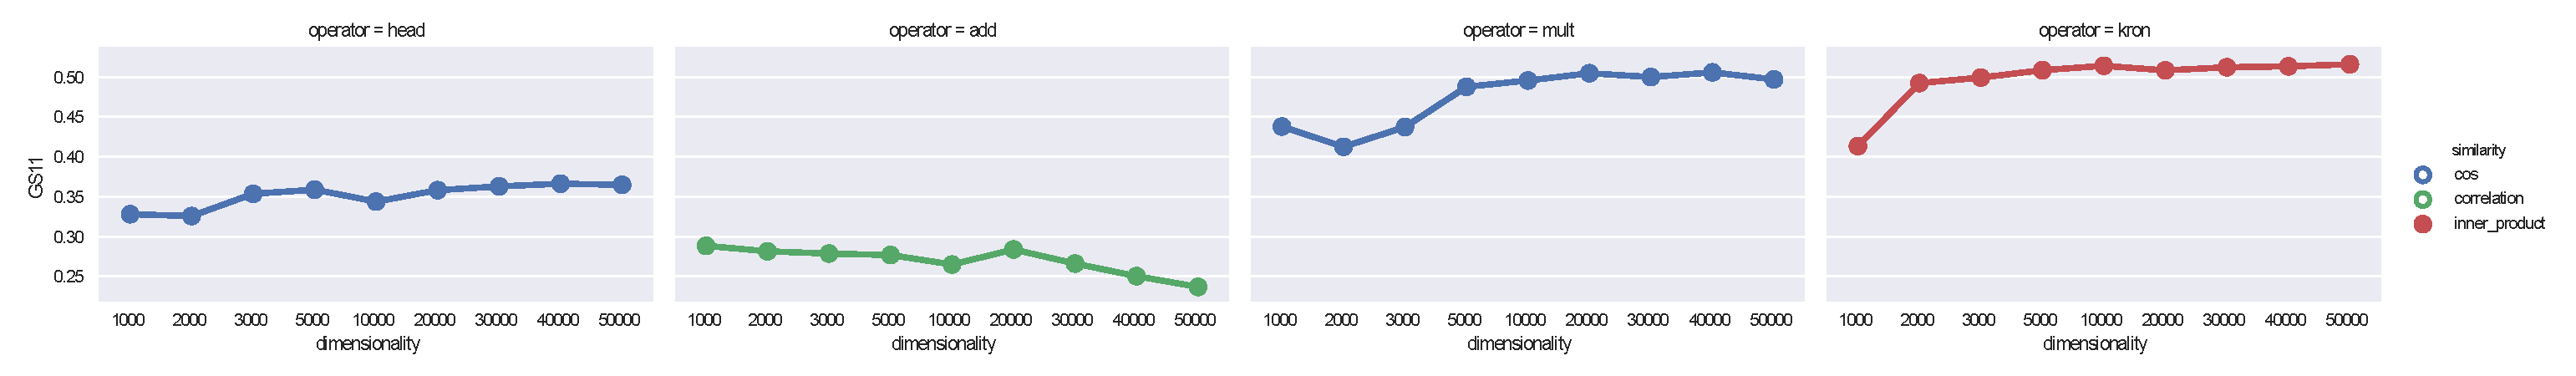
\includegraphics[width=\textwidth]{supplement/figures/GS11-heuristics-selection-similarity}
    \caption{H. Sim.}
    \label{fig:}
  \end{subfigure}

  \begin{subfigure}[t]{0.7\textwidth}
    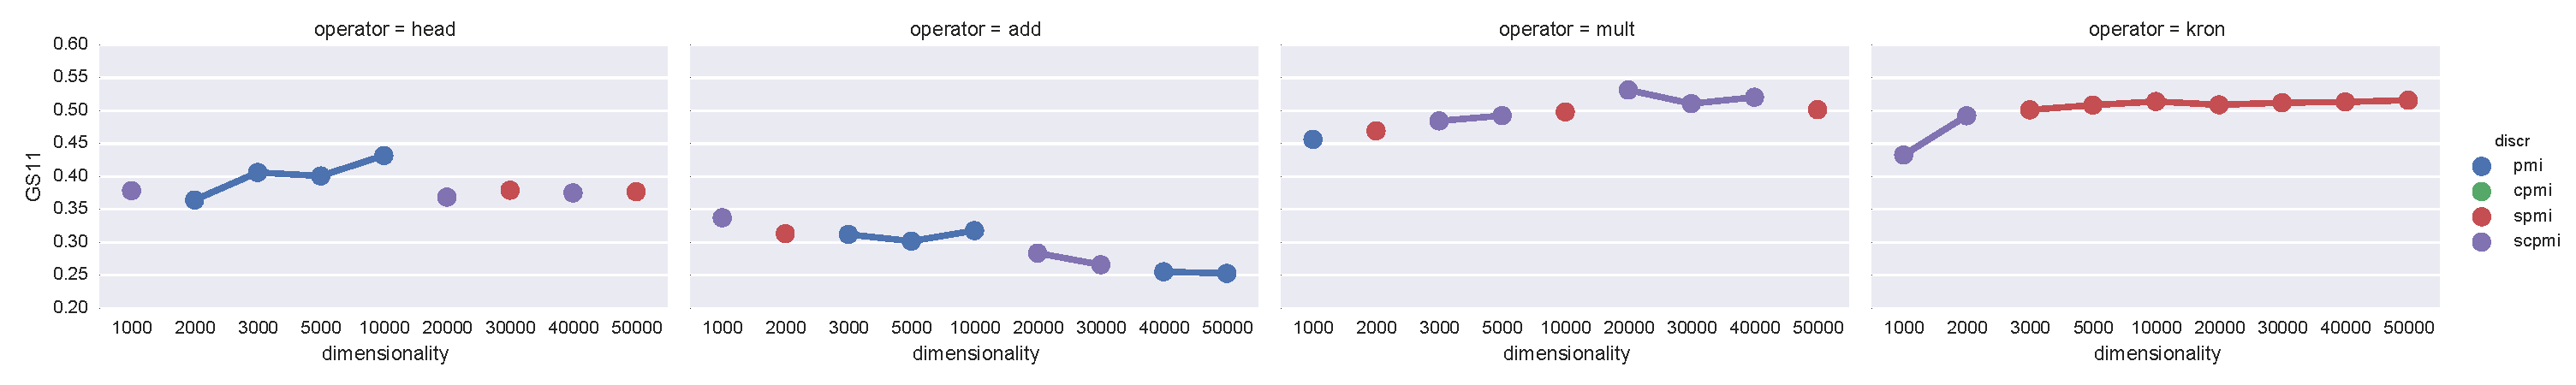
\includegraphics[width=\textwidth]{supplement/figures/GS11-max_-selection-discr}
    \caption{Max. Discr.}
    \label{fig:}
  \end{subfigure}
  % \begin{subfigure}[t]{0.7\textwidth}
  %   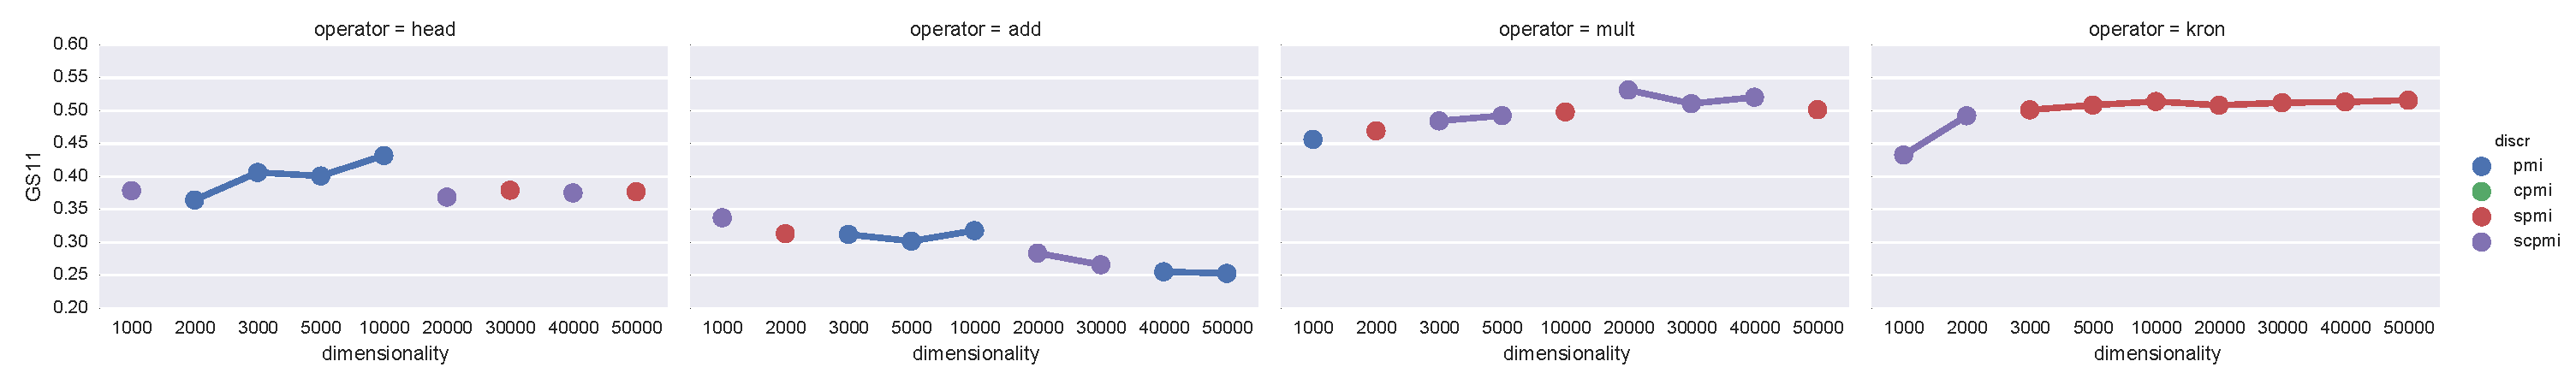
\includegraphics[width=\textwidth]{supplement/figures/GS11-cross_validation-selection-discr}
  %   \caption{CV. Discr.}
  %   \label{fig:}
  % \end{subfigure}
  \begin{subfigure}[t]{0.7\textwidth}
    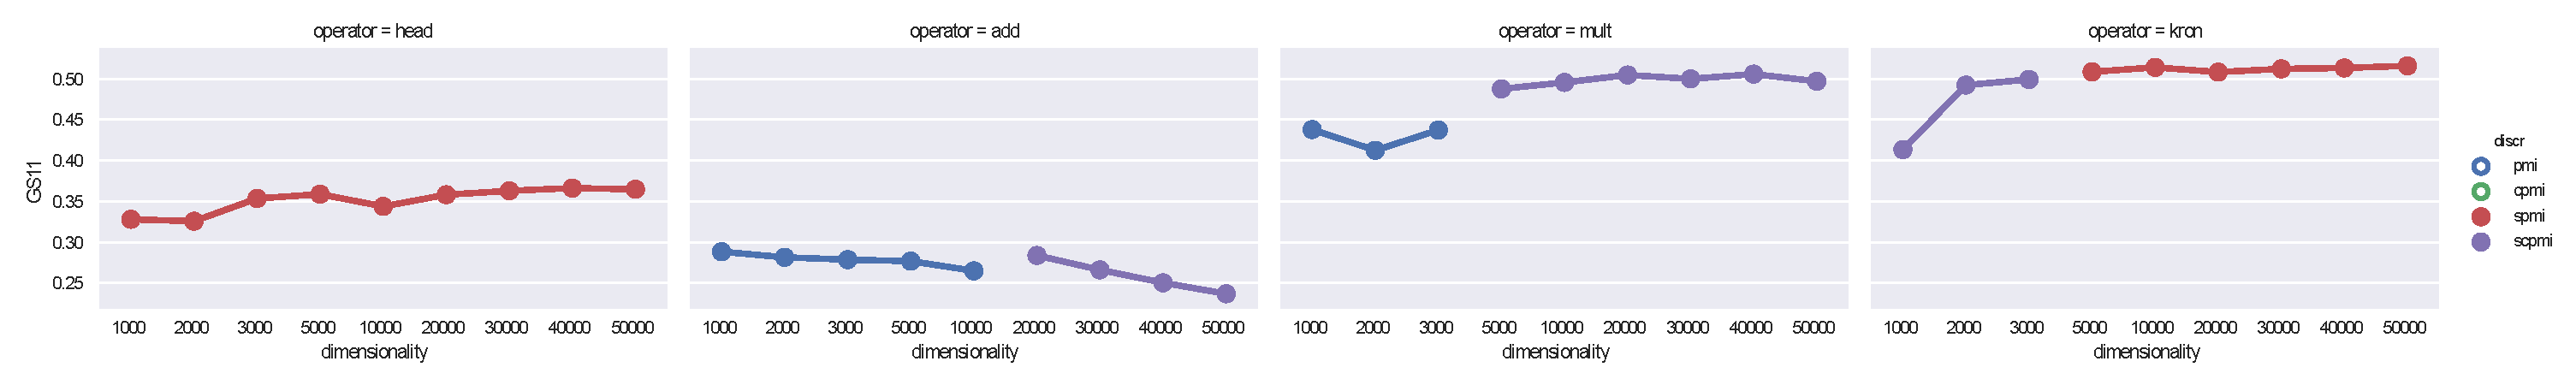
\includegraphics[width=\textwidth]{supplement/figures/GS11-heuristics-selection-discr}
    \caption{H. Discr.}
    \label{fig:}
  \end{subfigure}

  \caption{GS11 selection.}
  \label{fig:selection_gs11}
\end{figure}

\end{landscape}

\restoregeometry

% \clearpage
% \KOMAoptions{paper=A4,pagesize}
% \recalctypearea


% \subsection{GS12}
% \label{sec:gs12}

\subsection{Universal parameter selection for compositional datasets}
\label{sec:robust-param-comp-selecion}

\section{Universal parameter selection for lexical and compositional datasets}
\label{sec:universal-param-selection}



% \subsubsection{Tweaked IR evaluation}
% \label{sec:tweak-ir-eval}

% \todo[inline]{Discuss \cite{Milajevs:2015:IMN:2808194.2809448} and link to \ref{sec:phraserel}}

% \section{PhraseRel: relevance of sentences}
% \label{sec:sentential-relevance}

%%% Local Variables:
%%% mode: latex
%%% TeX-master: "thesis"
%%% End:

% \chapter{Issues with evaluation of distributional models}
% \label{cha:reflection}

% \section{Limitations of current similarity datasets}
% \label{sec:notion-similarity}

% In contrast to linguistic datasets which contain randomly paired words from a broad selection, datasets that come from psychology contain entries that belong to a single category such as \textit{verbs of judging} \cite{FILLENBAUM197454} or \textit{animal terms} \cite{HENLEY1969176}. The reason for category oriented similarity studies is that ``stimuli can only be compared in so far as they have already been categorised as identical, alike, or equivalent at some higher level of abstraction'' \cite{turner1987rediscovering}. Moreover, because of the \emph{extension effect} \cite{medin1993respects}, the similarity of two entries in a context is less than the similarity between the same entries when the context is extended. ``For example, \textit{black} and \textit{white} received a similarity rating of 2.2 when presented by themselves; this rating increased to 4.0 when \textit{black} was simultaneously compared with \textit{white} and \textit{red} (\textit{red} only increased 4.2 to 4.9)'' \cite{medin1993respects}. In the first case \textit{black} and \textit{white} are more dissimilar because they are located on the extremes of the greyscale, but in the presence of \textit{red} they become more similar because they are both monochromes.

% Both MEN and SimLex-999 provide pairs that do not share any similarity to control for false positives, and they do not control for the comparison scale. This makes similarity judgements ambiguous as it is not clear what low similarity values mean: incompatible notions or contrast in meaning. SimLex-999 assigns low similarity scores to the incompatible pairs (0.48, \textit{trick} and \textit{size}) and to antonymy (0.55, \textit{smart} and \textit{dumb}), but \textit{smart} and \textit{dumb} have relatively much more in common than \textit{trick} and \textit{size}!

\chapter{PhraseRel: an IR-inspired compositional dataset}
\label{sec:phraserel}

Datasets that quantify relationships between words have a long history.\footnotemark{} Some of the most well-known datasets are RG65 \cite{Rubenstein:1965:CCS:365628.365657}, WS353 \cite{2002:PSC:503104.503110}, BLESS \cite{baroni-lenci:2011:GEMS}, MEN \cite{Bruni:2014:MDS:2655713.2655714} and SimLex-999 \cite{hill2014simlex}. All of them have been applied to evaluate the distributional models of meaning.

\footnotetext{This chapter addresses the evaluation concerns stated in \newcite{Milajevs:2015:IMN:2808194.2809448}, which was presented at ICTIR 2015. The dataset and all referred data files are available at \url{\BASEURL}.}

Naturally, the idea of capturing lexical relationships was extended to phrases and sentences. Many phrase and sentence datasets exist, such as the MS Paraphrase Corpus \cite{dolan2005par} or the phrase entailment dataset of \newcite{baroni-EtAl:2012:EACL2012}. These are potentially applicable to evaluating compositional distributional models. We say potentially because the grammar-preserving compositional settings \cite{baroni2014frege,DBLP:journals/corr/abs-1003-4394}  rely on high dimensional tensor spaces which do not, at the moment, scale up to  the complex syntactic structures of such datasets. Instead, a family of phrasal, mostly \emph{similarity}-oriented datasets \cite{mitchell-lapata:2008:ACLMain,Grefenstette:2011:ESC:2145432.2145580,kartsaklis-sadrzadeh:2013:EMNLP,kartsadrqpl2014} are widely used for the evaluation of these models, see, for example, \citet{kim-demarneffe-foslerlussier:2015:VSM-NLP}.

We extend the possibility of evaluating compositional distributional models by proposing a task and a corresponding dataset  with controlled syntax. The task focuses on \emph{relevance}, a notion from Information Retrieval (IR).  Further, this task will assist with the understanding of how compositional distributional  models  can be used in IR, without limiting the choice of compositional methods. Much of the original research in distributional semantics has stemmed from vector models of IR, but the IR-NLP connection has been less apparent in  the newer compositional distributional models; our work attempts to bring them back together.

\newcite{Milajevs:2015:IMN:2808194.2809448} got promising results when testing distributional methods in an IR-inspired setting, improving over an IR baseline. However, that work was based on a \emph{similarity} rather than relevance gold standard with a tweaked evaluation method.

To overcome that flaw, we introduce a dataset that measures relevance. To develop the dataset, we took the  dataset of \newcite{kartsaklis-sadrzadeh:2013:EMNLP,kartsadrqpl2014} as the base, extensively extended it with query-document phrase pairs and re-annotated it using Amazon Mechanical Turk, asking for relevance judgements.

Due to the novelty of the method used in the creation of the dataset (which makes it to measure relevance rather than similarity), the effort dedicated to it and since is yet unpublished, we devote a separate chapter to explain it.

\section{Preparation of candidate entries for the dataset}
\label{sec:design}

As the base, we took the 72 unique sentences from the dataset of \newcite{kartsaklis-sadrzadeh:2013:EMNLP,kartsadrqpl2014}, which is later referred to as \emnlp/.\footnotemark{} These sentences formed the candidate \emph{query sentences}. We paired each query sentence with 23 \emph{document sentences} obtained by four conceptually different methods. Note that even though similarity is different from relevance, it has been used in the IR setting---see for example \newcite{2016arXiv160801972K}.
%
\footnotetext{\url{http://compling.eecs.qmul.ac.uk/wp-content/uploads/2015/07/KS2014.txt}}

\begin{figure*}
  \centering
  \tiny
  \begin{tabular}{lllllllllll}
    \toprule
    \multicolumn{3}{c}{Query} &
    \multicolumn{3}{c}{Document} &
    \multirow{2}{*}{Method} &
    \multicolumn{3}{c}{Relevance} &
    \multirow{2}{*}{Diverse}
    % \multirow{2}{*}{Diverse query}
    \\
    \cmidrule(r){1-3} \cmidrule(r){4-6} \cmidrule(r){8-10}
    Subject  & Verb & Object   & Subject  & Verb   & Object & &
    Mean & Std. & Type & \\
    \midrule
    delegate & buy  & land     & agent    & sell      & property & ks14 &
    1.33 & 1.53 & strict & false  \\
    agent & sell & property &
    delegate       & buy       & land       & ks14       &
    2.00  & 1.00 & strict & false \\

    agent & sell & property &
    representative & exchange  & possession & wordnet:hyper &
    1.00  & 1.73 & N/A & false    \\


    agent & sell & property &
    deputy         & trade     & estate     & wordnet:hypo  &
    1.00  & 0.00 & loose & false  \\

    agent & sell & property &
    people         & buy       & home       & frequency:0   &
    1.33  & 1.53 & strict & false \\

    agent & sell & property &
    company        & offer     & product    & frequency:1   &
    -2.00 & 1.73 & N/A & false    \\

    agent & sell & property &
    people         & advertise & product    & frequency:2   &
    -2.00 & 1.00 & N/A & false    \\

    agent & sell & property &
    family         & buy       & home       & selection     &
    -1.33 & 1.53 & N/A & false    \\

    agent & sell & property &
    company        & specify   & need       & selection     &
    -3.00 & 0.00 & N/A & false    \\

    agent & sell & property &
    people         & represent & set        & selection     &
    -3.00 & 0.00 & N/A & false    \\

    student & acquire & skill &
    student        & gain      & experience & selection     &
    2.00    & 1.00 & strict & true \\
  \bottomrule
  \end{tabular}
  \caption{An Example of query-document pairs}
  \label{fig:emnlp-pairing}
\end{figure*}


%%% Local Variables:
%%% mode: latex
%%% TeX-master: "../thesis"
%%% End:


\subsection{Entries taken from the \emnlp/ dataset}

Each query sentence is paired with a counterpart sentence from the high similarity band\footnotemark{} in the \emnlp/ dataset by treating the similarity band assignments as symmetric. For example, given a \emnlp/ combination
%
\footnotetext{%
The \emnlp/ dataset consists of three bands of intended similarity:
\begin{compactitem}
\item high similarity \dataurl{emnlp2013_turk_HighSim.txt},
\item medium similarity \dataurl{emnlp2013_turk_MedSim.txt},
\item low similarity \dataurl{emnlp2013_turk_LowSim.txt}.
\end{compactitem}
}
%
\begin{eqnarray*}
(\textmd{agent}, \textmd{sell}, \textmd{property}),
(\textmd{delegate}, \textmd{buy}, \textmd{land})
\end{eqnarray*}
%
in the high similarity band, we generated two query-document permutations listed
in Figure~\ref{fig:emnlp-pairing} with the method labelled as \texttt{ks14}.

\subsection{Entries generated from WordNet}
We generated two more document sentences for each query based on \emph{hyponymy} and \emph{hypernymy} relations from WordNet \cite{Miller:1995:WLD:219717.219748}. For each query sentence, one document sentence was manually generated by substituting the words of a sentence with their \emph{hypernymy} and another document sentence was obtained using \emph{hyponymy}.

During the manual process of retrieving hypernymy and hyponymy, we noticed that some were very good, for instance, \textit{datum}: \textit{information} and \textit{statistics}. However, some candidates were problematic, such as \textit{party}: \textit{political unit} and \textit{communist party} because we were looking for single words rather than phrases. In such cases, we dropped adjectives and adverbs or ignored a candidate. Two instances of WordNet-based sentence generation are shown in Figure~\ref{fig:emnlp-pairing} with the method set to \texttt{wordnet:hyper} and \texttt{wordnet:hypo}.

\subsection{Entries generated using ukWaC phrase frequencies}

To generate more document sentences we used a dependency-parsed version of ukWaC \cite{ukwac}. We extracted all possible subject-verb-object triplets from the corpus with their frequencies. Then, to generate document sentences for a query, we extracted candidate subjects, verbs and objects independently.

Consider that we need to extract candidate objects for the phrase \textit{agent sell property}. We retrieve objects of the 10 most frequent triplets with the same subject and object. In case there are less triplets like this, we retrieve additional subjects of the most frequent triplets that share only the subject or only the verb to fetch 10 subjects in total, giving preference to more frequent triplets. Candidate subjects and verbs are obtained in the same way.

Once candidate subjects, verbs and objects are fetched, we ranked all possible combinations of them by the frequency of appearance in ukWaC and select the top 7 triplets. Documents generated in this manner are labeled as \texttt{frequency:*} in Figure~\ref{fig:emnlp-pairing}, where the numbers are the frequency ranks of the triplets.

\subsection{Semantically similar entries}

To obtain more query-document pairings, we computed the cosine similarity of all queries and documents generated by the model based on  the SPMI weighting, $k=1$, with multiplicative composition. We appended 13 more documents most similar to a corresponding query to each query-document pool. In Figure~\ref{fig:emnlp-pairing} these pairs are labeled as \texttt{selection}.

We had 23 unique documents (1 \texttt{ks14}, 2 \texttt{wordnet}, 7
\texttt{frequency} and 13 \texttt{selection}) for each of the 72 queries, making
1656 query-document pairs to be evaluated by humans.

\section{Human evaluation}
\label{sec:human-evaluation}

\begin{figure}
\centering
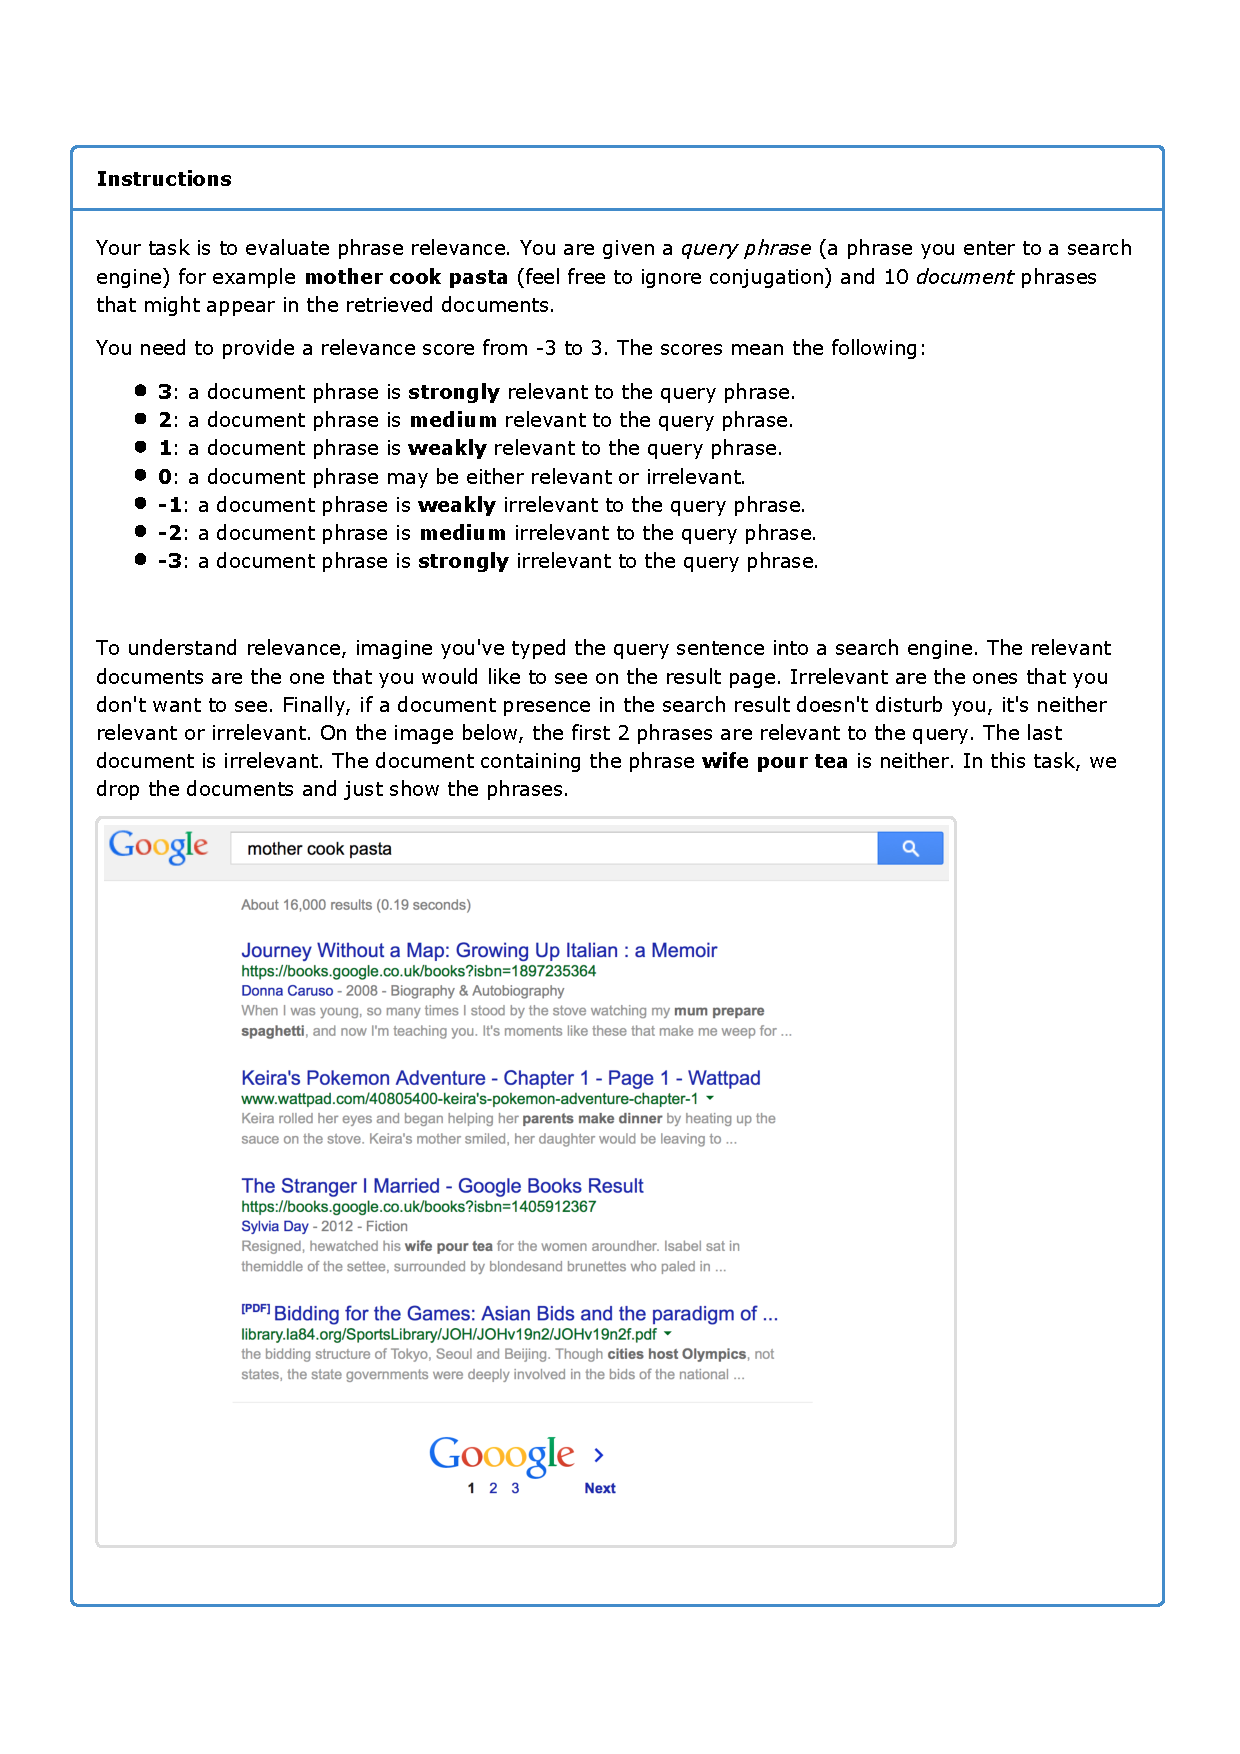
\includegraphics[width=0.9\textwidth]{figures/instructions}

\caption{Instructions given to the Mechanical Turkers}

\label{fig:instructions}
\end{figure}

%%% Local Variables:
%%% mode: latex
%%% TeX-master: "../paper.tex"
%%% End:


We recruited 19 human subjects using the Amazon Mechanical Turk platform.\footnote{\url{https://requester.mturk.com/}} Before answering a question, the subjects were given the instructions shown in Figure~\ref{fig:instructions}.

Each query-document pair was judged by three different people. The data was collected in two batches. Each question (or a HIT, Human Intelligence Task, in the Mechanical Turk terminology) consisted of a query phrase and 20 document sentences for the first batch and 10 documents for the second batch. Documents were shuffled before being shown to a human subject. Each document had to be judged for relevance using the following scoring system:
\begin{compactitem}
\item \textbf{-3}: strong irrelevance,
\item \textbf{-2}: medium irrelevance,
\item \textbf{-1}: weak irrelevance,
\item  \textbf{0}: a document may be either relevant or irrelevant,
\item  \textbf{1}: weak relevance,
\item  \textbf{2}: medium relevance,
\item  \textbf{3}: strong relevance.
\end{compactitem}

An example question is shown in Figure~\ref{fig:task}. The \dataurl{phraserel-raw.csv} file consists of human judgements together with anonymized Worker and HIT identifiers.

\begin{figure}
\centering
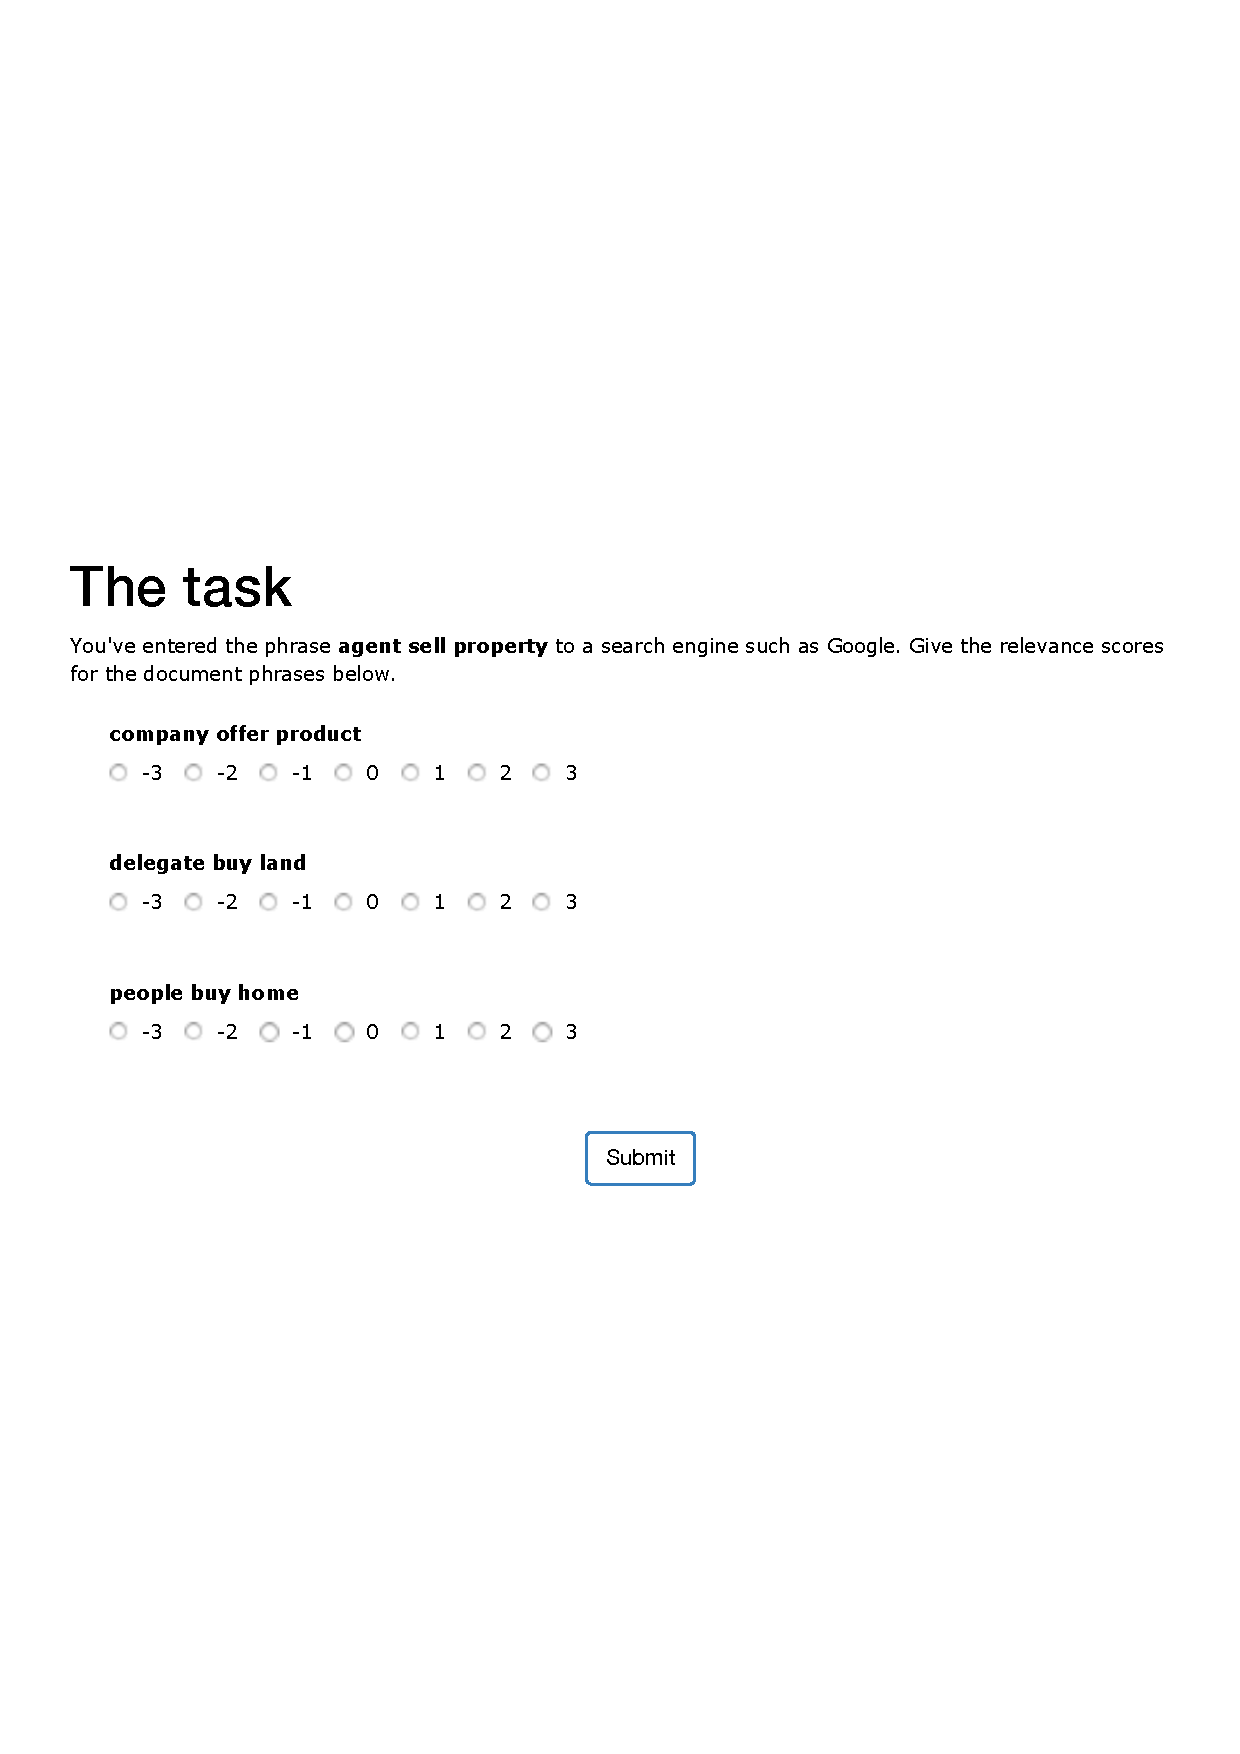
\includegraphics[width=0.9\textwidth]{figures/task}

\caption{\textbf{A sample question.}}

\label{fig:task}
\end{figure}

%%% Local Variables:
%%% mode: latex
%%% TeX-master: "../paper.tex"
%%% End:


\section{Final dataset construction}
\label{sec:postprocessing}

\subsection{Pair classification}

The pairs have been classified by the individual relevance judgements. A pair is of the \textit{strict relevance} type if all human judgements are greater than or equal to 0 and there is at least one 3 (strong relevance). A pair of the \textit{loosely   relevant} type is a pair where all human judgements are greater than or equal to 0. Figure~\ref{fig:emnlp-pairing} shows the mean and standard deviation of human judgements per query-document pair and the relevance division of a pair if applicable. There are 110 (or 7\%) strictly relevant pairs and 221 (13\%) loosely relevant pairs.
% * <sdyck@ualberta.ca> 2016-11-04T13:35:55.761Z:
%
% >  greater than or equal to 0
%
% but no 3's? otherwise loosely and strictly relevant classifications would overlap (all strictly would also be loosely) if that makes sense. 
%
% ^.

\subsection{Query classification}

Each query has been classified by the number of strictly relevant documents it has been paired with. On average, each query in the dataset is paired with 3.3 loosely relevant and 1.6 strictly relevant documents. The minimum number of loosely relevant documents per query is 1, the maximum is 14. Regarding the strict relevance, there are 8 queries without a single strictly relevant document, and the maximum number of strictly relevant documents per query is 7.

A query is \textit{diverse} if it is paired with 4 or more loosely relevant documents. There are 28 (42\%) such queries. On average, diverse queries are paired with 5.2 loosely relevant documents and 2.4 strictly relevant documents.
% \begin{compactitem}
% \item 14 queries with 4 loosely relevant documents,
% \item 6 with 5,
% \item 5 with 6,
% \item 1 with 7,
% \item 1 with 9,
% \item 1 with 14.
% \end{compactitem}

%%% Local Variables:
%%% mode: latex visual-line
%%% TeX-master: "thesis"
%%% TeX-engine: xetex
%%% End:

\chapter{Relationships between sentences}
\label{sec:sentential}

\lettrine[lines=5,loversize=0.25]{I}{n} this chapter, we study the relationship between lexical representations and various methods of composition and look for the optimal lexical representations for additive, multiplicative and Kronecker-based compositional methods.\footnotemark{} We do not make any assumption regarding lexical representations and test all of them to see their behavioural patterns in compositional setting.

\footnotetext{This chapter includes the results presented in \newcite{milajevs-EtAl:2014:EMNLP2014} at EMNLP 2014.}

Here we report the results on the compositional datasets KS14 \cite{kartsadrqpl2014}, GS11 \cite{Grefenstette:2011:ETV:2140490.2140497} and PhraseRel (Chapter~\ref{sec:phraserel}). For the first two datasets, the evaluation is done similarly to the lexical evaluation (Chapter~\ref{sec:lexical}) by computing Sperman-$\rho$ rank correlation between human judgements and model estimation. If a dataset provides several human judgements for a sentence pair, the judgements are averaged before computing the correlation. For PhraseRel, we report relevant@3, the measure that is the proportion of sentences for which the top-3 most similar neighbours contain at least one sentence that was judged relevant with respect to the source sentence.

We show that the optimal choice of lexical parameters depends on the method of composition, so, for example, with addition the vectors that are used with addition should be sparser then the vectors that are used with multiplication and Kronecker. We also show that the parameter choice optimal in lexical tasks is sub-optimal in compositional tasks especially for multiplication and Kronecker. 

\section{Experiments on KS14 dataset}
\label{sec:ks14}

KS14 is a sentence similarity dataset prepared by \citet{kartsadrqpl2014}. It consists of pairs of transitive sentences that are judged by similarity. The goal is to achieve high correlation with human judgements in predicting sentential similarity. We also report behaviour of a baseline operator \texttt{head}, which ignores the subject and the object of a sentence and makes the vector of a sentence equal to the vector of the head word, in our case the verb.

\subsection{Max selection}
\label{sec:max-selection-ks14}

Figure~\ref{fig:ks14-results} shows the performance of compositional models on the sentence similarity dataset KS14. All operators outperform the non-compositional \texttt{head} operator. Table~\ref{tab:ks14-max-selection} shows the performance of models selected by Max selection together with the selected parameters.

% \todo[noline]{Significance test}
Kronecker with a few thousand dimensions and correlation as the similarity measure gives the highest scores, supporting H\ref{hyp:order} that word order is important in predicting similarity. As the dimensionality increases, Kronecker performance stays constant. Addition is slightly better than multiplication, but the performance of both peaks at 2\,000 dimensions and decreases as dimensionality increases.

\begin{figure}[b]
  \centering

    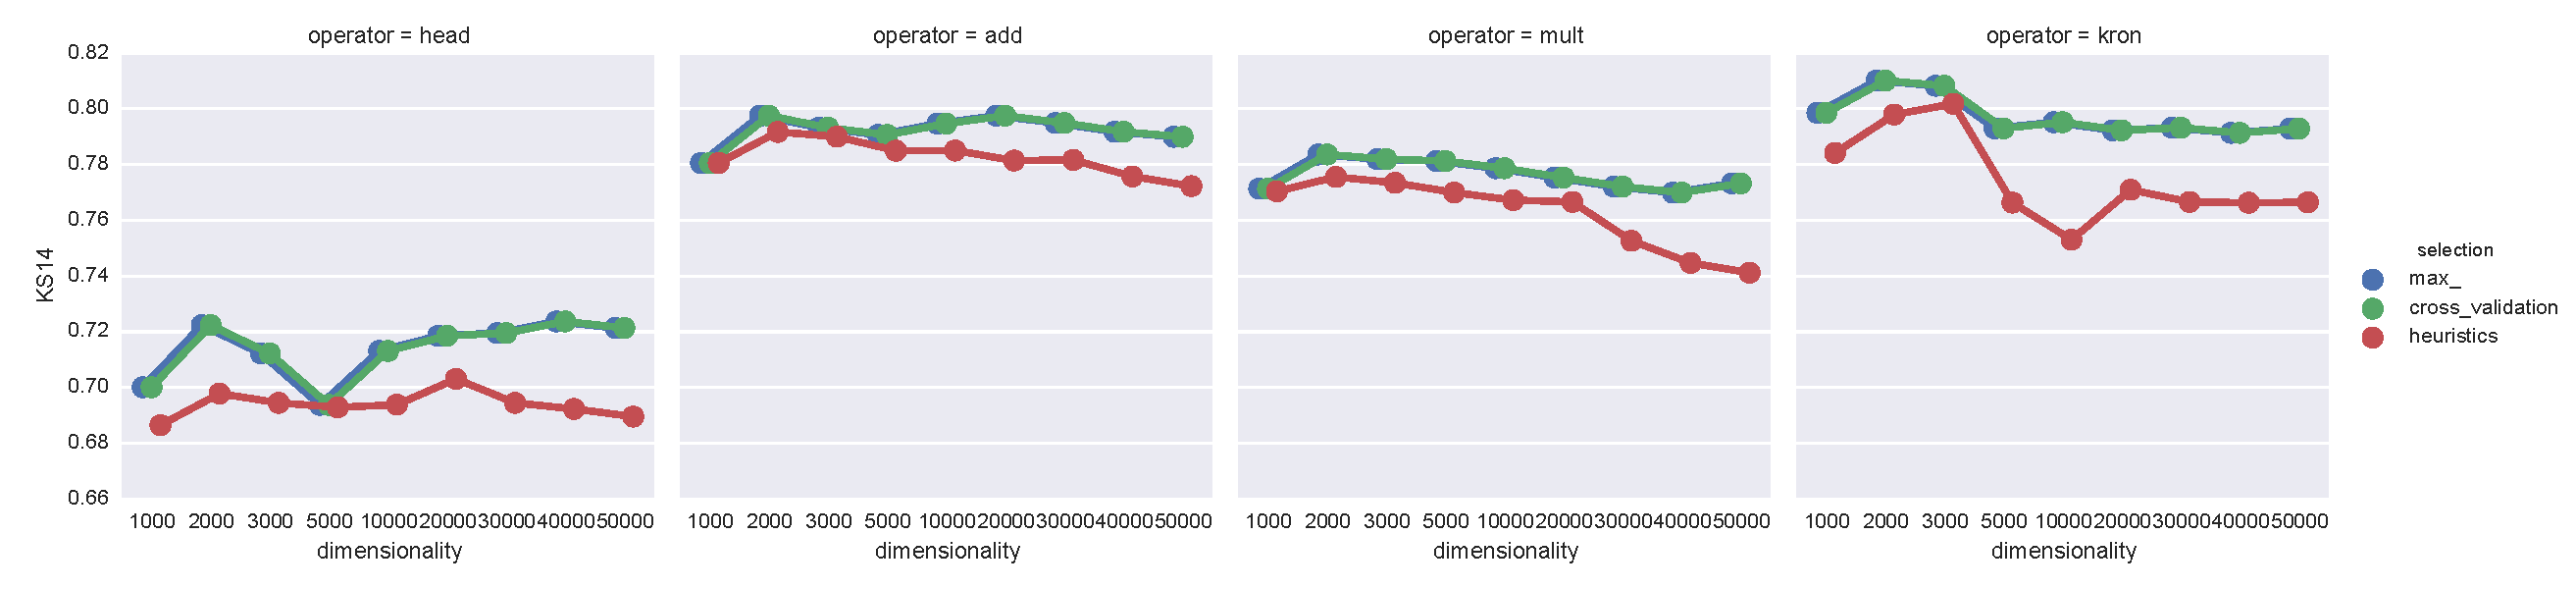
\includegraphics[width=\textwidth]{supplement/figures/ks14-results}
  \caption{KS14 results.}
  \label{fig:ks14-results}
\end{figure}

%%% Local Variables:
%%% mode: latex
%%% TeX-master: "../thesis"
%%% End:


Parameters of the baseline compositional method \texttt{head} are similar to the lexical Max selection (Table~\ref{tab:lexical-max-selection}), with an exception of \texttt{neg}, which controls vector sparsity, where higher values that are similar to MEN (Table~\ref{tab:men-max-selection}) are chosen.

All compositional operators agree in the choice of \texttt{freq} ($\log n$), \texttt{discr} (SCPMI) and similarity (correlation---note that Kronecker was tested only with the inner product for $D > 3\,000$ because of limited computational resources).

Compositional operators perform best with constant \texttt{freq} of 1, in contrast to the lexical setting, where $\log n$ is more beneficial. This might be because during composition the $\log n$ term dominates over the PMI value and minimises its effect.

Local context probabilities perform better in compositional tasks then in lexical tasks. Multiplication benefits from the unsmoothed distribution probability, while high-dimensional models perform best with smoothing ($\alpha = 0.75$), supporting H\ref{hyp:cds} that context smoothing is needed only for high-dimensional models. The only exceptions are additive models with $D < 5\,000$, where global probabilities perform best.

For low-dimensional spaces, addition performs best with sparse spaces ($k > 1$, $D < 5\,000$), but for high-dimensional spaces, addition performs best  with dense spaces ($k = 0,7$, $D \geq 5\,000$). This is against H\ref{hyp:neg} that states the opposite.

Multiplication, independently of dimensionality, performs best with dense spaces ($k = 0.2$).

Kronecker---in contrast to addition---performs best with dense low-dimensional models ($k = 0.2$, $D < 5\,000$) and sparser high-dimensional models ($k = 0.7$, $D \geq 5\,000$), which complies with H\ref{hyp:neg}. However, this difference might be explained by the change of the similarity measure, which is the inner product for $D \geq 5\,000$.

\subsection{Heuristics}
\label{sec:heuristics}

\begin{wraptable}[11]{O}{0.5\textwidth}
  %\vspace{-10pt}
  \centering

  \begin{tabular}{lr}
\toprule
      parameter &  partial $R^2$ \\
\midrule
            neg &  0.331 \\
           freq &  0.307 \\
       operator &  0.305 \\
            cds &  0.136 \\
     similarity &  0.061 \\
          discr &  0.054 \\
 dimensionality &  0.034 \\
\bottomrule
\end{tabular}


  \caption{KS14 feature ablation}
  \label{tab:ks14-ablation}
\end{wraptable}


The linear model achieves an $R^2$ of 0.794. The partial $R^2$s are shown in Table~\ref{tab:ks14-ablation}. The most influential parameters are \texttt{neg}, \texttt{freq}, compositional operator and \texttt{cds}. Interestingly, similarity has much less influence on this compositional dataset than on lexical datasets, where for Sim-Lex-999 (Table~\ref{tab:SimLex999-ablation}) and combined (Table~\ref{tab:lexical-ablation}) it is the most influential parameter. Also, note that dimensionality has the lowest partial $R^2$.

\subsubsection{Shifting}

For the baseline operator \texttt{head}, the best shifting choice of $k$ is 1 for spaces with dimensionality less than 5\,000 (Figure~\ref{fig:ks14-neg}). For $5\,000 \leq D < 30\,000$, \texttt{head} behaves best with $k = 1.4$. For $D \geq 3\,000$, $k$ should be set to 2.

For addition, spaces with $D < 20\,000$ should be used with $k = 1.4$, and with $k = 2$ otherwise.

For multiplication, there are three most beneficial choices: for $D < 10\,000$ $k = 0.5$, for $10\,000 \leq D < 30\,000$ $k = 0.7$ and, finally, for $D > 30\,000$ $k = 1$.

Kronecker shows a behaviour  similar to multiplication for $k$ as dimensionality increases, but prefers sparser spaces. For $D < 3\,000$: $k = 0.5$, for $3\,000 \leq D < 20\,000$: $k = 0.7$ and for $20\,000 \leq D$: $k = 1$.

All operators behave in accordance to H\ref{hyp:neg} that low-dimensional spaces benefit from being dense, while high-dimensional spaces benefit from being sparse.

\begin{figure}
% \begin{wrapfigure}{O}{0.5\textwidth}
  % \vspace{-30pt}
  \centering

  \begin{subfigure}[t]{\textwidth}
    \includegraphics[width=1.1\textwidth]{supplement/figures/ks14-interaction-neg}

  \caption{\texttt{neg}}
  \label{fig:ks14-neg}
  \end{subfigure}

  \begin{subfigure}[t]{\textwidth}
    \includegraphics[width=1.1\textwidth]{supplement/figures/ks14-interaction-freq}

  \caption{\texttt{freq}}
  \label{fig:ks14-freq}
  \end{subfigure}

  \caption{KS14.}
\end{figure}


\subsubsection{Frequency}
The best option of frequency for the baseline operator \texttt{head} is $\log n$ (Figure~\ref{fig:ks14-freq}). The constant frequency 1 is very close to $\log n$, but its performance declines for spaces with $D > 20\,000$.

For addition, frequency should be set to 1 for spaces with $D < 5\,000$ and to $\log n$ otherwise.

There is one choice of frequency for multiplication: 1. However, $\log n$ behaves similarly to it when $D \geq 3\,000$.

Kronecker follows addition with regard to frequency, but the split point is $D = 10\,000$: low-dimensional spaces should be used with constant frequency 1, and high-dimensional spaces with $\log n$.

Generally, H\ref{hyp:freq}---that non-constant frequency is beneficial for high-dimensional spaces---is supported by all operators in this dataset.

\subsubsection{Context distribution smoothing}

\begin{figure}
% \begin{wrapfigure}{O}{0.5\textwidth}
  % \vspace{-30pt}
  \centering

  \begin{subfigure}[t]{\textwidth}
    \includegraphics[width=1.1\textwidth]{supplement/figures/ks14-interaction-cds}

  \caption{\texttt{cds}}
  \label{fig:ks14-cds}
  \end{subfigure}

  \begin{subfigure}[t]{\textwidth}
    \includegraphics[width=1.1\textwidth]{supplement/figures/ks14-interaction-similarity}

  \caption{\texttt{similarity}}
  \label{fig:ks14-similarity}
  \end{subfigure}

  \caption{KS14.}
\end{figure}

The baseline operator \texttt{head} with spaces with dimensionality less than 20\,000 should be used with global probabilities, and more dimensional models should be used with smoothed local probabilities: $\alpha = 0.75$ (Figure~\ref{fig:ks14-cds}).

All other operators perform best with global context probability. Even though local context probability with $\alpha = 1$ is close to global, H\ref{hyp:cds} is not supported by this dataset: context distribution smoothing does not affect high-dimensional spaces.

\subsubsection{Similarity}
The baseline operator \texttt{head} on spaces with $D < 20\,000$ performs best with cosine similarity, while more dimensional models prefer correlation as the similarity measure (Figure~\ref{fig:ks14-similarity}), strictly according to H\ref{hyp:similarity}: the adjustment by the mean value that is performed by correlation is need by high-dimensional models.

Other operators work best with correlation. Addition and multiplication also support H\ref{hyp:similarity}. In the case of multiplication, correlation dominates over cosine, even for small values of $D$. There is little to say about Kronecker, as it is tested only with the inner product for spaces with $D > 3\,000$, due to its computational complexity ($\mathcal{O}(n^2)$ with respect to the number of vector components).

\subsubsection{Discriminativeness}

\begin{figure}[b]
% \begin{wrapfigure}{O}{0.5\textwidth}
  % \vspace{-30pt}
  \centering

  \includegraphics[width=1.1\textwidth]{supplement/figures/KS14-interaction-discr}

  \caption{KS14 influence of \texttt{discr}}
  \label{fig:ks14-discr}
\end{figure}

The baseline operator \texttt{head} with $D < 20\,000$ prefers SCPMI as the discriminativeness weighting. SPMI is preferred otherwise (Figure~\ref{fig:ks14-discr}).

For addition, SPMI is the better choice. For multiplication, SCPMI is more beneficial, as expected by H\ref{hyp:comp-pmi-cpmi}: the compression of PMI values improves performance of compositional models.

For Kronecker, the two choices are very close to each other. For spaces with dimensionality less than 20\,000, SPMI is slightly better; for spaces with greater dimensionality---SCPMI.

\subsection{Difference between Max selection and heuristics on KS14}

Table~\ref{tab:ks14-heuristics-selection} shows the selection based on heuristics, which is more homogeneous than the selection based on the highest score (Table~\ref{tab:ks14-max-selection}). Both methods agree on the similarity choice (with the exception of \texttt{head}).

Multiplication agrees on the majority of parameters, except \texttt{cds} and \texttt{neg}. Local probabilities ($\alpha = 1$) and $k = 0.2$ give the highest score, while manual selection picked global context probabilities with \texttt{neg} in the range of 0.5 to 1, in accordance with H\ref{hyp:neg} that high-dimensional spaces should be sparser.

The average difference between Max and heuristic-based selections is 0.022. Per operator, the differences are: 0.028 (\texttt{head}), 0.012 (addition), 0.018 (multiplication) and 0.028 (Kronecker). All values are within the 10\% set by H\ref{hyp:10percent}.

\section{Experiments on GS11 dataset}
\label{sec:gs11}

GS11 is a dataset of transitive sentences \cite{Grefenstette:2011:ESC:2145432.2145580,Grefenstette:2011:ETV:2140490.2140497}. It consists of ambiguous transitive verbs together with their arguments and two landmark verbs that each disambiguate a particulate sense of the ambiguous verb. Human judgements provide pairwise similarity scores between the sentence with the ambiguous verb and the two sentences with the landmark verbs.

\subsection{Max selection}
\label{sec:max-selection-gs11}

\begin{figure}[b]
  \centering

    \includegraphics[width=\textwidth]{supplement/figures/gs11-results}
  \caption{GS11 results.}
  \label{fig:gs14-results}
\end{figure}

%%% Local Variables:
%%% mode: latex
%%% TeX-master: "../thesis"
%%% End:


Figure~\ref{fig:gs14-results} shows performance of the compositional models on the verb disambiguation task. Table~\ref{tab:gs11-max-selection} shows the selected model performance together with chosen parameters.

Multiplication with 20\,000 dimensions gives the highest result of 0.532. Kronecker gets close with a score of 0.516 with $D = 50\,000$, giving no support to H\ref{hyp:order} that word order is important for similarity measurement. Addition does not outperform the baseline \texttt{head} operator: addition scores 0.338, while \texttt{head}'s best performance is 0.432.

The behaviour of the baseline operator \texttt{head} is unstable for dimensions less than 20\,000, and its best behaviour might be the case of overfitting similarly with SimLex-999. However, models with dimensions greater than 20\,000 yield similar scores, even though the parameters are different.

In general, Max parameter selection is very different than the one based on KS14 (Table~\ref{tab:ks14-max-selection}). Compositional operators behave best with $\log n$ frequency, especially Kronecker. PMI often outperforms other discriminativeness components in the case of \texttt{head} and addition. Global context probability estimation behaves better than local and correlation is not always the best similarity measure.

Addition's behaviour degrades as dimensionality increases, whereas multiplication behaviour increases, but becomes unstable for spaces with more than 20\,000 dimensions. Kronecker depends the least on the dimensionality.

Addition works best with dense models. Multiplication and Kronecker prefer dense, low-dimensional spaces and sparse, high-dimensional spaces, supporting H\ref{hyp:neg} that a frequency component is required for high-dimensional spaces.

\subsection{Heuristics}
\label{sec:heuristics-gs11}

The linear model achieves an $R^2$ of 0.753. The partial $R^2$ scores are shown in Table~\ref{tab:gs11-ablation}. The most influential parameters are a compositional operator, \texttt{freq} and \texttt{neg}. This is the same as in the case of KS14, but in reverse order (Table~\ref{tab:ks14-ablation}).

\subsubsection{Frequency}

\begin{wraptable}[8]{O}{0.5\textwidth}
% \begin{table}[b]
  \vspace{-4em}
  \centering
  \begin{tabular}{lr}
\toprule
      parameter &  partial $R^2$ \\
\midrule
       operator &  0.37 \\
           freq &  0.21 \\
            neg &  0.18 \\
     similarity &  0.09 \\
            cds &  0.05 \\
          discr &  0.04 \\
 dimensionality &  0.04 \\
\bottomrule
\end{tabular}


  \caption{GS11 feature ablation}
  \label{tab:gs11-ablation}
\end{wraptable}

On average, $\log n$ behaves best for all operators (Figure~\ref{fig:gs11-freq}). For $D \leq 5\,000$, 1 is also a good frequency choice, supporting H\ref{hyp:freq} that non-constant frequency component is required for high-dimensional spaces.

\subsubsection{Shifting}

The baseline operator \texttt{head} on average works best with shifted models. For models with dimensionality less than 3\,000, $k = 0.5$ is best, otherwise $k = 0.7$ is more beneficial (Figure~\ref{fig:gs11-neg}).

For addition, models without shifting behave best for $D < 20\,000$, however, for more dimensional spaces, $k = 0.2$ should be preferred. This is a weak support of H\ref{hyp:neg} (high-dimensional vectors should be sparse), because unshifted spaces can be seen as shifted with a very small $\alpha$ value.

Multiplication also works best with unshifted low-dimensional spaces ($D < 5\,000$) and with $k = 0.7$ for high-dimensional spaces, supporting H\ref{hyp:neg}.

Kronecker prefers shifting. For spaces with dimensionality less then 20\,000 $k = 0.7$ and $k = 1$ otherwise. This is inline with H\ref{hyp:neg}.

\begin{figure}
% \begin{wrapfigure}{O}{0.5\textwidth}
  % \vspace{-30pt}
  \centering

  \begin{subfigure}[t]{\textwidth}
    \includegraphics[width=1.1\textwidth]{supplement/figures/GS11-interaction-freq}

  \caption{\texttt{freq}}
  \label{fig:gs11-freq}
  \end{subfigure}

  \begin{subfigure}[t]{\textwidth}
    \includegraphics[width=1.1\textwidth]{supplement/figures/GS11-interaction-neg}

  \caption{\texttt{neg}}
  \label{fig:gs11-neg}
  \end{subfigure}

  \caption{GS11 influence of \texttt{freq} and \texttt{neg}}
\end{figure}


\subsubsection{Similarity}

The baseline operator \texttt{head} and multiplication work best with cosine similarity, addition with correlation and Kronecker with inner product (Figure~\ref{fig:gs11-similarity}).

Addition strictly supports H\ref{hyp:similarity} that cosine is optimal for high-dimensional spaces, while multiplication supports it by behaving similarly to cosine and correlation.

\subsubsection{Context distribution smoothing}

The baseline operator \texttt{head} with $D < 10\,000$ works best with global context probabilities. For more dimensional spaces, local context probabilities $\alpha = 1$ should be preferred (Figure~\ref{fig:gs11-cds}).

Addition works best with local probabilities. In the low-dimensional case, when $D < 20\,000$, unsmoothed estimation ($\alpha = 1$) is preferred and $\alpha = 0.75$ should be chosen otherwise.

Multiplication works best with global context probabilities and Kronecker with smoothed local ($\alpha = 0.75$).

There is no support of H\ref{hyp:cds} (context distribution smoothing leads to optimal results with high-dimensional models) because global context probabilities outperform other choices for multiplication, addition behaves the same with all options and Kronecker works best with $\alpha = 0.75$.

\begin{figure}
% \begin{wrapfigure}{O}{0.5\textwidth}
  % \vspace{-30pt}
  \centering

  \begin{subfigure}[t]{\textwidth}
    \includegraphics[width=1.1\textwidth]{supplement/figures/gs11-interaction-similarity}

  \caption{Similarity}
  \label{fig:gs11-similarity}
  \end{subfigure}

  \begin{subfigure}[t]{\textwidth}
    \includegraphics[width=1.1\textwidth]{supplement/figures/gs11-interaction-cds}

  \caption{\texttt{cds}}
  \label{fig:gs11-cds}
  \end{subfigure}

  \caption{GS11.}
\end{figure}


\subsubsection{Discriminativeness}

\begin{figure}[b]
% \begin{wrapfigure}{O}{0.5\textwidth}
  % \vspace{-30pt}
  \centering

  \includegraphics[width=1.1\textwidth]{supplement/figures/GS11-interaction-discr}

  \caption{GS11 \texttt{discr}}
  \label{fig:gs11-discr}
\end{figure}


The baseline operator \texttt{head} works best with SPMI, but SCPMI is very close (Figure~\ref{fig:gs11-discr}). Addition works best with PMI for $D < 20\,000$ and SCPMI otherwise.

Multiplication is similar to addition in that it prefers PMI in the low-dimensional case and SCPMI in the high-dimensional case, but the change happens at 5\,000 dimensions rather than 20\,000.

Kronecker with less than 5\,000 dimensions prefers SCPMI and SPMI, which is opposite to addition and multiplication.

This dataset does not give evidence to support H\ref{hyp:comp-pmi-cpmi}---PMI values should be compressed when used in compositional setting---because there is almost no difference betwen *PMI and *CPMI.

\subsection{Difference between Max selection and heuristics on GS11}

Only logarithmic frequency component ($\log n$) was chosen by heuristics (Table~\ref{tab:gs11-heuristics-selection}), while there is a mix of 1 and $\log n$ in the Max selection (Table~\ref{tab:gs11-max-selection}).

Kronecker and most of multiplication's discriminativeness choices agree, while for \texttt{head} and addition there is little agreement between parameter selection. The same goes for context distribution smoothing and shifting.

Similarity choice is the same for Kronecker and addition, but \texttt{head} and multiplication---according to heuristics---should be used with cosine similarity, while there is no single metric that leads to maximum performance.

The overall average normalised difference in results between Max and heuristic-based selections is 0.054. Per operator, the differences are: 0.090 \texttt{head}, 0.077 addition, 0.043 multiplication and 0.006 Kronecker. All the values are within the 10\% boundary set by H\ref{hyp:10percent}.

\section{Experiments on PhraseRel dataset}
\label{sec:phraserel-experiment}

PhraseRel is a dataset that is built for evaluation of distributional models, but instead of similarity judgements, relevance judgements are provided. The evaluation measure is relevance@3. This is the proportion of the retrieval results for which there is a relevant document among the top three ranked documents.

\subsection{Max selection}
\label{sec:max-selection-phraserel}

\begin{figure}
  \centering

    \includegraphics[width=\textwidth]{supplement/figures/phraserel-results}
  \caption{PhraseRel results.}
  \label{fig:phraserel-results}
\end{figure}

%%% Local Variables:
%%% mode: latex
%%% TeX-master: "../thesis"
%%% End:


Figure~\ref{fig:phraserel-results} shows the performance of the models on the PhraseRel dataset. All operators outperform the non-compositional \texttt{head} baseline. Table~\ref{tab:phraserel-max-selection} shows the models that yield the best result together with model parameters.

Multiplication, in general, outperforms all other operators, and with the dimensions of 10\,000 and 20\,000, gets the perfect score of 1. The fact that Kronecker (a word order sensitive operator) is outperformed by multiplication (a word order insensitive operator) gives no support of H\ref{hyp:order} that word order matters. Model performance weakly depends on the dimensionality for all operators. Multiplication and Kronecker show strong performance similarly to the preliminary study, where similarity was assumed to correspond to relevance \cite{Milajevs:2015:IMN:2808194.2809448}.

Addition and Kronecker achieve the best score with constant frequency, \texttt{head} works best with linear and multiplication with sublinear ($\log n$) frequency.

SPMI is the preferred discriminativeness component for the low-dimensional spaces ($D < 10\,000$) for the baseline \texttt{head}, otherwise, SCPMI is the best behaving \texttt{discr}. For addition and the spaces with $D > 1\,000$, SPMI is the best, while for the spaces with the same dimensionality, multiplication prefers CPMI, which is in line with H\ref{hyp:comp-pmi-cpmi}: PMI values should be compressed when used in compositional tasks. Kronecker, most of the time, prefers SCPMI.

The baseline operator \texttt{head} with dimensions less than 20\,000 works best with local smoothed context probabilities, however, for more dimensional spaces, global context probabilities are more competitive. On the contrary, addition prefers smoothed local context probabilities for spaces with dimensions more than 5\,000. Multiplication exhibits different pattern: when a model contains few dimensions, it prefers local, smoothed context probabilities, and for high-dimensional spaces it prefers local, but unsmoothed context probabilities, which goes against H\ref{hyp:cds} (context distribution smoothing should be optimal with high-dimensional spaces). Kronecker is inconsistent with regards to the choice of \texttt{cds}, but for models with $D \geq 30\,000$, global context probabilities perform the best.

Regarding shifting, the baseline operator \texttt{head} prefers sparse spaces $k > 1$, but as dimensionality increases, the optimal $k$ values decrease. Addition does not show a consistent behaviour with regard to this parameter. Multiplication, in general, benefits from dense, unshifted spaces. Kronecker works best with sparse spaces with increasing sparsity as the dimensionality increases, supporting H\ref{hyp:neg}: low-dimensional models should be dense, but high-dimensional models should be sparse.

The baseline operator \texttt{head} benefits from the correlation as the similarity measure, as does multiplication. Addition works best with correlation with spaces $D < 10\,000$, and with the inner product for more dimensional spaces. Multiplication works best with correlation. Kronecker, for spaces with less than 5\,000 dimensions, works best with correlation and with the inner product, otherwise.

\subsection{Heuristics}
\label{sec:heuristics-phraserel}

\begin{wraptable}[10]{O}{0.5\textwidth}
% \begin{table}[b]
  \vspace{-1em}
  \centering

  \begin{tabular}{lr}
\toprule
      parameter &  partial $R^2$ \\
\midrule
            neg &       0.58 \\
       operator &       0.35 \\
            cds &       0.08 \\
           freq &       0.04 \\
     similarity &       0.03 \\
 dimensionality &       0.03 \\
          discr &       0.02 \\
\bottomrule
\end{tabular}


  \caption{PhraseRel feature ablation}
  \label{tab:phraserel-ablation}
\end{wraptable}


The linear model achieves an $R^2$ of 0.822. The partial $R^2$ scores are shown in Table~\ref{tab:phraserel-ablation}. The most influential parameters are \texttt{neg}, operator and \texttt{cds}, but the first two have partial $R^2$ scores much higher than the other parameters. Table~\ref{tab:phraserel-heuristics-selection} shows the performance of the chosen models.

\subsubsection{Shifting}
\label{sec:shifting-phraserel}

The baseline operator \texttt{head} should be used with $k = 1.4$, addition should be used with $k = 2$ and multiplication should be used with $k = 0.5$ (Figure~\ref{fig:phraserel-neg}).

Kronecker has three optimal values of $k$ that are proportional to dimensionality. For models with dimensionality less than 5\,000, $k = 0.5$ is preferred; for $5\,000 \leq D < 20\,000$, the most beneficial choice of \texttt{neg} is $k = 1$; finally, for spaces with more than 20\,000 dimensions, $k$ should be set to 1.4. This supports H\ref{hyp:neg} that model sparsity should increase as dimensionality increases.

\begin{figure}
% \begin{wrapfigure}{O}{0.5\textwidth}
  % \vspace{-30pt}
  \centering

  \begin{subfigure}[t]{\textwidth}
    \includegraphics[width=1.1\textwidth]{supplement/figures/phraserel-interaction-neg}

  \caption{\texttt{neg}}
  \label{fig:phraserel-neg}
  \end{subfigure}

  \begin{subfigure}[t]{\textwidth}
    \includegraphics[width=1.1\textwidth]{supplement/figures/phraserel-interaction-cds}

  \caption{\texttt{cds}}
  \label{fig:phraserel-cds}
  \end{subfigure}

  \caption{PhraseRel.}
\end{figure}


\subsubsection{Context distribution smoothing}
\label{sec:cont-distr-smooth-phraserel}

The best choice for the baseline operator \texttt{head} deponds on dimensionality: spaces with less than 10\,000 dimensions benefit from smoothed local context probabilities ($\alpha = 0.75$) (Figure~\ref{fig:phraserel-cds}). Addition and multiplication work best with global context probabilities, while Kronecker prefers unsmoothed local probabilities ($\alpha = 1$).

\subsubsection{Frequency}
\label{sec:frequency-phraserel}

The baseline operator\texttt{head} works best with linear frequency, but the difference between other options is small (Figure~\ref{fig:phraserel-freq}). Addition benefits from linear frequency, but sublinear frequency is very close. Multiplication works best with sublinear frequency, but linear is very close to it. Finally, Kronecker works best with $\log n$ with spaces with dimensionality less than 5\,000, and with linear frequency with more dimensional spaces.

In general, H\ref{hyp:freq} (non-linear frequency should be used with high-dimensional spaces) holds, because there is no difference between 1 and $\log n$ choices in model performance.

\begin{figure}[b]
% \begin{wrapfigure}{O}{0.5\textwidth}
  % \vspace{-30pt}
  \centering

  \begin{subfigure}[t]{\textwidth}
    \includegraphics[width=1.1\textwidth]{supplement/figures/phraserel-interaction-freq}

  \caption{\texttt{freq}}
  \label{fig:phraserel-freq}
  \end{subfigure}

  \begin{subfigure}[t]{\textwidth}
    \includegraphics[width=1.1\textwidth]{supplement/figures/phraserel-interaction-similarity}

  \caption{similarity}
  \label{fig:phraserel-similarity}
  \end{subfigure}

  \caption{PhraseRel.}
\end{figure}


\subsubsection{Similarity}
\label{sec:similarity-phraserel}

For all operators, there is little difference between cosine and correlation, weakly supporting H\ref{hyp:similarity} that correlation should be used with high-dimensional spaces and cosine with low-dimensional spaces.

The baseline operator \texttt{head} works best with correlation as the similarity measure with models with $D < 5\,000$, and with cosine for more dimensional ones (Figure~\ref{fig:phraserel-similarity}). Note, however, that the difference between the two is very small.

Addition benefits from cosine when $D < 20\,000$ and from inner product otherwise. But, in the case of addition, all three similarity measures are close to each other.

Multiplication works best with correlation. Where tested, correlation behaves best with Kronecker.

\subsubsection{Discriminativeness}
\label{sec:discriminativeness-phraserel}

\begin{figure}[b]
% \begin{wrapfigure}{O}{0.5\textwidth}
  % \vspace{-30pt}
  \centering

  \includegraphics[width=1.1\textwidth]{supplement/figures/phraserel-interaction-discr}

  \caption{PhraseRel \texttt{discr}}
  \label{fig:phraserel-discr}
\end{figure}


The baseline \texttt{head} prefers different discriminativeness components depending on dimensionality. For models with $D < 5\,000$, SPMI is the best, while for other dimensions SCPMI is more competitive.

Addition and Kronecker benefit from SPMI, and multiplication from SCPMI, apart from the dimensionality of 10\,000. H\ref{hyp:comp-pmi-cpmi}, that PMI compression improves results in compositional tasks, is only supported by multiplication.

\subsection{Difference between Max selection and heuristics on PhraseRel}
\label{sec:diff-phraserel}

Manual parameter selection is more stable than the one based on the maximum values. However, in cases where different parameters are picked, there is little or no difference between these parameter choices. For example studied similarity measures yield similar average performance for addition, see Figure~\ref{fig:phraserel-freq}.

Manual heuristics do not pick the best result of 1 (Table~\ref{tab:phraserel-max-selection}), but are close with a multiplicative model with 20\,000 and 30\,000 dimensions, yielding a score of 0.964 (Table~\ref{tab:phraserel-heuristics-selection}).

The average relative difference between the Max selection and the selection based on heuristics is 0.022 for \texttt{head}, 0.072 for addition, 0.041 for multiplication and 0.061 for Kronecker.

Over all compositional methods, the difference is 0.049, which is within the 10\% limit set by H\ref{hyp:10percent}.

\section{Selected model transfer across the datasets}
\label{sec:select-model-transf-comp}

\begin{figure}[t]
  \centering
    \includegraphics[width=\textwidth]{supplement/figures/KS14-transfer}
    \caption{Transfer from KS14.}
    \label{fig:ks14-transfer}
\end{figure}

%%% Local Variables:
%%% mode: latex
%%% TeX-master: "../thesis"
%%% End:


\subsection{Difference between heuristics}
\label{sec:diff-betw-heur-comp}

There is little agreement on parameter selection based on heuristics among the three compositional datasets. The only consistent choice is global context probability (\texttt{cds}) and SCPMI discriminativeness for multiplicative models.

There is more pairwise agreement, for example, similarity based on correlation for additive models on KS14 and GS11 and $\log n$ frequency for multiplicative models between GS11 and PhraseRel. The pairwise agreement might be a sign of overfitting, because there is no clear pattern. On the other side, the difference in performance between parameter choices might be negligible, as some parameters consistently show low $R^2$ scores, for example \texttt{discr}. Consequently, there is inconsistency in the supported hypotheses.

\subsection{Model transfer from KS14}
\label{sec:from-ks14}

Figure~\ref{fig:ks14-transfer} shows the behaviour of models selected on the KS14 when they are transferred to GS11 and PhraseRel. During the transfer, there is little difference in performance between the selection methods, except in multiplicative models where heuristics show better performance and 5\,000-dimensional Kronecker where heuristics give lower results than the Max-based selection.

Heuristic-based selection, on average, is closer to the upper bound than Max-based selection, supporting H\ref{hyp:overfitting} that Max selection overfits. However, both are beyond the 10\% boundary set by H\ref{hyp:10percent}. When transferred to GS11, the average difference with the upper bound is 0.335 for Max and 0.238 for heuristics. When transferred to PhraseRel the average difference is 0.093 for Max and 0.091 for heuristics.

\subsection{Model transfer from GS11}
\label{sec:from-gs11}

\begin{figure}
  \centering
    \includegraphics[width=\textwidth]{supplement/figures/GS11-transfer}
    \caption{Transfer from GS11}
    \label{fig:gs11-transfer}
\end{figure}

%%% Local Variables:
%%% mode: latex
%%% TeX-master: "../thesis"
%%% End:


Figure~\ref{fig:gs11-transfer} shows that there is little difference between Max and heuristic-based selections. In case of \texttt{head} composition, heuristics lead to higher performance, while for low-dimensional multiplicative models heuristics fall behind the Max selection on the KS14 dataset.

% \todo[noline]{Significance tests}
When GS11 models are transferred to KS14, the average difference with the upper bound is 0.119 and 0.106 for Max and heuristics respectively. For the transfer to PhraseRel, the differences are 0.133 for Max and 0.188 for heuristics. Again, the heuristic-based selection outperforms the Max based. This supports H\ref{hyp:overfitting} that Max selection overfits, but the results are beyond the limit of H\ref{hyp:10percent}.

\subsection{Model transfer from PhraseRel}
\label{sec:from-phraserel}

\begin{figure}
  \centering
    \includegraphics[width=\textwidth]{supplement/figures/PhraseRel-transfer}
    \caption{Transfer from Phraserel.}
    \label{fig:phraserel-transfer}
\end{figure}

%%% Local Variables:
%%% mode: latex
%%% TeX-master: "../thesis"
%%% End:


Figure~\ref{fig:phraserel-transfer} shows that the performance of models based on PhraseRel is less stable, especially for selection by maximum performance.

% \todo[noline]{Significance tests}
Transfer to KS14 yields the average differences of 0.152 for Max and 0.136 for heuristics. Transfer to GS11 yields the average differences of 0.454 for Max and 0.509 for heuristics. Note that the PhraseRel to GS11 transfer is the only case where Max selection, on average, is better than heuristics.

In general, over all compositional datasets, we see---in contrast to the lexical evaluation---that the Max-based selection might be prone to overfitting (H\ref{hyp:overfitting}). However, the result difference is far beyond the 10\% limit set by H\ref{hyp:10percent}, which might be due to the different nature of the tasks: similarity, disambiguation and relevance (compositional) versus similarity and relatedness (lexical).

\section{Universal parameter selection for compositional datasets}
\label{sec:robust-param-comp-selecion}

Figure~\ref{fig:compositional-results} shows the performance of the models based on the combined selection over the KS14, GS11 and PhraseRel datasets. The combined score is calculated the following way:

{
\scriptsize
\begin{align}
\operatorname{score}_\mathit{compositional}&(\mathit{m}, \mathit{o}) =
&\frac{1}{3}\times%
\frac{\operatorname{score}_\mathit{KS14}(\mathit{m}, \mathit{o})}%
{\max_m\operatorname{score}_\mathit{KS14}(m, \mathit{o})}%
+%
\frac{1}{3}\times%
\frac{\operatorname{score}_\mathit{GS11}(\mathit{m}, \mathit{o})}%
{\max_m\operatorname{score}_\mathit{GS11}(m, \mathit{o})}%
+%
\frac{1}{3}\times%
\frac{\operatorname{score}_\mathit{PhraseRel}(\mathit{m, \mathit{o}})}%
{\max_m\operatorname{score}_\mathit{PhraseRel}(m, \mathit{o})}%
\end{align}
%\normalsize
}
where $m$ is a model and $o$ is an operator.

The performance of selected models together with the selected parameters is shown in Table~\ref{tab:compositional-max-selection} (Max selection) and Table~\ref{tab:compositional-heuristics-selection} (selection based on heuristics).

\begin{figure}
  \centering

  \begin{subfigure}[t]{\textwidth}
    \includegraphics[width=\textwidth]{supplement/figures/compositional-results-ks14}
    \caption{KS14.}
    \label{fig:compositional-results-ks14}
  \end{subfigure}

  \begin{subfigure}[t]{\textwidth}
    \includegraphics[width=\textwidth]{supplement/figures/compositional-results-gs11}
    \caption{GS11.}
    \label{fig:compositional-results-gs11}
  \end{subfigure}

  \begin{subfigure}[t]{\textwidth}
    \includegraphics[width=\textwidth]{supplement/figures/compositional-results-phraserel}
    \caption{PhraseRel.}
    \label{fig:compositional-results-phraserel}
  \end{subfigure}


  \caption{Performance of models based on the selection over the average compositional performance.}
  \label{fig:compositional-results}
\end{figure}

%%% Local Variables:
%%% mode: latex
%%% TeX-master: "../thesis"
%%% End:


\subsection{Max selection}
\label{sec:max-selection-compositional}

Models with many dimensions do not always perform better than their low-dimensional counterparts. Particularly, only \texttt{head} and multiplication benefit from the high number of dimensions. Addition and Kronecker are closer to the upper bound with dimensionality of a few thousand.

Regarding the hypotheses, there is support of H\ref{hyp:freq} (non-constant frequency should be used with high-dimensional spaces) for addition, multiplication and Kronecker, H\ref{hyp:cds} (context distribution smoothing is optimal for high-dimensional spaces) for multiplication and H\ref{hyp:neg} (low-dimensional spaces should be dense, high-dimensional---sparse) for Kronecker.

\subsection{Heuristics}
\label{sec:heuristics-compositional}

\begin{wraptable}[6]{O}{0.5\textwidth}
% \begin{table}
  \vspace{-5em}
  \centering

  \begin{tabular}{lr}
\toprule
      parameter &  partial $R^2$ \\
\midrule
            neg &           0.40 \\
           freq &           0.29 \\
       operator &           0.21 \\
            cds &           0.15 \\
     similarity &           0.08 \\
          discr &           0.06 \\
 dimensionality &           0.05 \\
\bottomrule
\end{tabular}


  \caption{Compositional feature ablation}
  \label{tab:compositional-ablation}
\end{wraptable}


The linear model achieves  $R^2 = 0.769$. Table~\ref{tab:compositional-ablation} shows the partial $R^2$ values for the parameters. The most influential parameters are \texttt{neg}, \texttt{freq} and compositional operator.

\subsubsection{Neg}
\label{sec:neg-compositional}

\begin{figure}
% \begin{wrapfigure}{O}{0.5\textwidth}
  % \vspace{-30pt}
  \centering

  \begin{subfigure}[t]{\textwidth}
    \includegraphics[width=1.1\textwidth]{supplement/figures/compositional-interaction-neg}

  \caption{\texttt{neg}}
  \label{fig:compositional-neg}
  \end{subfigure}

  \begin{subfigure}[t]{\textwidth}
    \includegraphics[width=1.1\textwidth]{supplement/figures/compositional-interaction-freq}

  \caption{\texttt{freq}}
  \label{fig:compositional-freq}
  \end{subfigure}

  \caption{Compositional.}
\end{figure}


For \texttt{head} and models with $D < 10\,000$, the \texttt{neg} should be set to 1, otherwise, it should be 1.4 (Figure~\ref{fig:compositional-neg}).

For addition, 1 is the best choice of \texttt{neg}, but the performance of $k$ values follows H\ref{hyp:neg}.

Multiplication benefits from denser spaces. If the dimensionality is less than 10\,000, then \texttt{neg} should be set to 0.5, otherwise 0.7 is a good choice, confirming H\ref{hyp:neg}.

Kronecker benefits from the \texttt{neg} of 0.7 if $D < 10\,000$ and from 1 for the more dimensional cases, supporting H\ref{hyp:neg}. This is similar to multiplication, but Kronecker prefers less dense vectors.

\subsubsection{Freq}
\label{sec:freq-compositional}

The frequency value of choice of all operators is $\log n$ with an exception of multiplication, where the constant frequency is preferred (Figure~\ref{fig:compositional-freq}).
% * <sdyck@ualberta.ca> 2016-11-05T00:53:40.350Z:
%
% > $\log n$ is
%
% rearrange so the sentence doesn't start with a lowercase
% DM: done.
% ^.

For low-dimensional vector spaces ($D \leq 5\,000$), 1 behaves good giving support of H\ref{hyp:freq}.
% * <sdyck@ualberta.ca> 2016-11-05T00:54:01.016Z:
%
% > 1 behav
%
% rearrange so that sentence doesn't start with a number
% DM: done.
% ^.

\subsubsection{Context distribution smoothing}
\label{sec:cont-distr-smooth-compositional}

\begin{figure}[b]
% \begin{wrapfigure}{O}{0.5\textwidth}
  % \vspace{-30pt}
  \centering

  \begin{subfigure}[t]{\textwidth}
    \includegraphics[width=1.1\textwidth]{supplement/figures/compositional-interaction-cds}

  \caption{\texttt{cds}}
  \label{fig:compositional-cds}
  \end{subfigure}

  \begin{subfigure}[t]{\textwidth}
    \includegraphics[width=1.1\textwidth]{supplement/figures/compositional-interaction-similarity}

  \caption{Similarity}
  \label{fig:compositional-similarity}
  \end{subfigure}

  \caption{Compositional influence of \texttt{cds} and similarity}
\end{figure}


As Figure~\ref{fig:compositional-cds} shows, global context probability is the preferred choice of context probability in all cases, with an exception of Kronecker with $D > 3\,000$, where smoothed local probabilities are better ($\alpha = 0.75$), supporting H\ref{hyp:cds}.

\subsubsection{Similarity}
\label{sec:similarity-compositional}

Correlation is the dominant choice of the similarity measure (Figure~\ref{fig:compositional-similarity}). However, cosine is preferred in the case of \texttt{head}, with $D > 5\,000$, and inner product is the only choice for composition with Kronecker with $D > 3\,000$.

There is no distinction between cosine and correlation for all compositional operators, which neither supports nor disputes H\ref{hyp:similarity}.
% * <sdyck@ualberta.ca> 2016-11-05T00:55:26.642Z:
%
% > es not contradict H
%
% does not contradict is not necessarily the same as support. So are you saying it neither supports nor disputes H13?
% DM: yes.
% ^.

\subsubsection{Discr}
\label{sec:discr-compositional}

\begin{figure}
% \begin{wrapfigure}{O}{0.5\textwidth}
  % \vspace{-30pt}
  \centering

  \includegraphics[width=1.1\textwidth]{supplement/figures/compositional-interaction-discr}

  \caption{Compositional influence of \texttt{discr}}
  \label{fig:compositional-discr}
\end{figure}


SPMI is the choice of \texttt{discr} that leads to the best average performance in most cases (Figure~\ref{fig:compositional-discr}). However, the difference between SPMI and SCPMI is very small.

The exceptions are Multiplicative composition with $D \geq 10\,000$ and Kronecker with $D \leq 5\,000$ where SCPMI outperforms SPMI, as expected by H\ref{hyp:comp-pmi-cpmi} that PMI values compression is needed for composition.

\subsection{Comparison with the selection based on one dataset}
\label{sec:comp-with-single-comp}

Manual selection based on a combination of the compositional datasets is more stable with regards to the chosen parameter values than the selection based on the highest values, even though manual selection does not always achieve the performance of Max selection, see Figure~\ref{fig:compositional-results}.

The average difference with the upper bound is 0.040 and 0.041 for Max and heuristics, respectively, when applied to KS14. For GS11, the difference is 0.045 (Max) and 0.127 (Heuristics). For PhraseRel, the difference is 0.055 (Max) and 0.084 (Heuristics).

The numbers are much lower than the transfer of spaces selected on the basis of one dataset (Section~\ref{sec:select-model-transf-comp}). The average normalised difference is within the 10\% limit (H\ref{hyp:10percent}), with an exception of heuristics on GS11. This is evidence that there might be one universal model that fits various tasks (H\ref{hyp:universal}). The fact that the average normalised difference is smaller for Max-based selection is against H\ref{hyp:overfitting}. A combination of datasets that covers several phenomena (in our case, similarity, disambiguation and relatedness) might be more effective than manual heuristic-based selection.

The model selection procedures improve from the combination of datasets. One needs to keep in mind that in this case we test model performance on the same dataset as we do parameter selection.

\section{Conclusion}
\label{sec:conclusion-comp}

Phrasal experiments support most of the hypotheses stated in
Section~\ref{sec:hypotheses}.

The confirmation of hypotheses on optimal parameter dependence on dimensionality (in particular H\ref{hyp:freq} (\texttt{freq}) and H\ref{hyp:neg} (\texttt{neg}), that are supported by all datasets) confirms H\ref{hyp:dimen}. It is worth noting that even though an optimal choice of \texttt{cds} does not depend on dimensionality on KS14 and GS11, in the combined case the dependence holds.

Models that are selected on the experiments on a single dataset are prone to overfitting. Neither manual selection of parameters prevents it and the average normalised difference is above 10\% on model transfer. This confirms H\ref{hyp:overfitting} and rejects H\ref{hyp:10percent}.

Model selection based on the combination of datasets performs much better on each dataset (contrary to a single-dataset selected models). Both selection methods are within 10\%, supporting H\ref{hyp:10percent}.

Max selection models outperform heuristic selection models, suggesting that there is no overfitting in this case and H\ref{hyp:overfitting} is not valid. In this case, the dataset combination covered three phenomena (similarity, disambiguation and relevance) and the precaution of overfitting by heuristics might be redundant.

This also suggests that there is a unique parameter choice that is universally applicable to compositional tasks H\ref{hyp:universal}. The universal spaces are studied in Chapter~\ref{sec:universal-param-selection}.

\chapter[Universal models]{Universal models for both lexical and compositional tasks}
\label{sec:universal-param-selection}

\lettrine[lines=5,loversize=0.25]{T}{his} chapter investigates how well one model can perform on all tasks in contrast to the task-tailored models of previous chapters.
% This is achieved by performing the evaluation on a combined score over the previous two lexical and three phrasal datasets.
We not only combine the datasets together, but also look for parameters that are good across all datasets with all compositional operators. Once optimal parameters are identified, they are tested on categorical compositional methods.

Even though the identified parameters have to compromise over different tasks (lexical and compositional) and compositional methods we achieve the new state-of-the-art results with Kronecker on KS14 and GS11. Moreover, the selected lexical representations improve over the results of the categorical compositional methods reported in the literature.

\section{Operator-dependent universal models}
\label{sec:model-selection}

\subsection{Max selection}
\label{sec:max-selection-universal}

Table~\ref{tab:universal-max-selection} shows the performance of the models evaluated with a combined score of the lexical and compositional datasets. The combined score for a model and an operator is computed as:

{\scriptsize
  \begin{align}
    \begin{split}
\operatorname{score}_\mathit{universal}(\mathit{m}, \mathit{o}) = & %
\frac{1}{2}\times\left(
\frac{1}{2}\times%
\frac{\operatorname{score}_\mathit{SimLex-999}(\mathit{m})}%
{\max_m\operatorname{score}_\mathit{SimLex-999}(m)}%
+%
\frac{1}{2}\times%
\frac{\operatorname{score}_\mathit{MEN}(\mathit{m})}%
{\max_m\operatorname{score}_\mathit{MEN}(m)}%
\right) +
\\
&\frac{1}{2}\times\left(
\frac{1}{3}\times%
\frac{\operatorname{score}_\mathit{KS14}(\mathit{m}, \mathit{o})}%
{\max_m\operatorname{score}_\mathit{KS14}(m, \mathit{o})}%
+%
\frac{1}{3}\times%
\frac{\operatorname{score}_\mathit{GS11}(\mathit{m}, \mathit{o})}%
{\max_m\operatorname{score}_\mathit{GS11}(m, \mathit{o})}%
+%
\frac{1}{3}\times%
\frac{\operatorname{score}_\mathit{PhraseRel}(\mathit{m, \mathit{o}})}%
{\max_m\operatorname{score}_\mathit{PhraseRel}(m, \mathit{o})}%
\right)
\end{split}
\end{align}
% \normalsize
}

Parameter selection is much more stable than on all previous Max-based selections. The dominant \texttt{freq} choice is $\log n$, cosine is the measure of choice for multiplication and Kronecker (if available). Correlation is the best similarity measure for the additive composition. The optimal choice of a similarity measure does not depend on dimensionality---this observation does not support H\ref{hyp:similarity}.

Interestingly, when shifting is applied, dense spaces perform better: 1 and 0.7 are the optimal \texttt{neg} values. Multiplication  supports H\ref{hyp:neg}.

% \todo[noline]{This is one of the major findings.}
The preference of a compositional operator depends on a model. Addition with many dimensions gives the best results on lexical tasks: 0.384 on SimLex-999 and 0.761 on MEN. Kronecker, on the other side, gives the highest values on compositional datasets supporting H\ref{hyp:order}: 0.798 on KS14, 0.514 on GS11 and 0.964 on PhraseRel. Multiplication, however, is a good compromise between the two. It gives the highest ``combined'' score of 0.945.

\subsection{Heuristics}
\label{sec:heuristics-universal}

\begin{wraptable}[6]{O}{0.5\textwidth}
  \vspace{-7em}
  \centering

  \begin{tabular}{lr}
\toprule
      parameter &  partial $R^2$ \\
\midrule
           freq &       0.32 \\
            neg &       0.29 \\
     similarity &       0.22 \\
            cds &       0.10 \\
          discr &       0.09 \\
 dimensionality &       0.07 \\
       operator &       0.05 \\
\bottomrule
\end{tabular}


  \caption{Universal (operator dependent) feature ablation}
  \label{tab:universal-ablation}
\end{wraptable}


Performance of the models selected manually is shown in Table~\ref{tab:universal-heuristics-selection}. Again, there is a lot of consistency between parameters. The linear model achieves $R^2 = 0.828$. The most influencing parameters are \texttt{freq}, \texttt{neg} and a similarity measure. See Table~\ref{tab:universal-ablation} for more details.

Heuristics for addition choose models that score the highest on lexical tasks: 0.384 on SimLex-999 and 0.764 on MEN (Table~\ref{tab:universal-heuristics-selection}). Moreover, with more than 20\,000 dimensions, there is no difference between the selection procedures (Max or heuristics) of the additive and Kronecker-based models.

Kronecker is strong in compositional tasks scoring 0.795 on KS14, 0.516 on GS11 and 0.929 on PhraseRel, which is in line with H\ref{hyp:order} that word order is important (Table~\ref{tab:universal-heuristics-selection}).

Multiplication and Kronecker support H\ref{hyp:neg}: the optimal shifting value $k$ depends on the dimensionality. Addition and Kronecker are consistent with H\ref{hyp:cds}: low-dimensional spaces benefit from global context probabilities, while high-dimensional spaces benefit from smoothed context probabilities with $\alpha=0.75$.

Multiplication, again, is a compromise between the two: it gives the highest combined score of 0.941. The highest Kronecker's combined score is 0.913, while addition's highest score is only 0.843.

Regarding the hypotheses, we clearly see on Figure~\ref{fig:universal-freq} that there is little difference between 1 and $\log n$ frequencies for the low-dimensional spaces, but $\log n$ is the best choice for the high-dimensional spaces, which is consistent with H\ref{hyp:freq}.

Shifting performs also in accordance with H\ref{hyp:neg}: for low-dimensional spaces $k=0.7$ or even $k=0.5$ leads to the highest result, while for high-dimensional spaces $k=1$ or $k=1.4$ are optimal.

We also see that there is no difference between the cosine and correlation similarity measures giving a weak support of H\ref{hyp:similarity}.

Addition and Kronecker work best with global context probabilities on low-dimensional spaces, but benefit from local probabilities ($\alpha=0.75$) for high-dimensional spaces, supporting H\ref{hyp:cds}. Multiplication, however, does not follow H\ref{hyp:cds}, as $\alpha=0.75$ leads to weak performance for all dimensions.

There is no support of H\ref{hyp:comp-pmi-cpmi}: for all operators, there is little difference between SPMI and SCPMI.

\subsection{Comparison of the selection methods}
\label{sec:comparison-universal}

On lexical tasks, there is little difference between the model selection methods, especially for spaces with more than 30\,000 dimensions, as Figures~\ref{fig:universal-results-simlex} and \ref{fig:universal-results-men} show.

The average relative differences for Max selection are 0.034 (SimLex-999), 0.010 (MEN), 0.033 (KS14), 0.109 (GS11) and 0.061 (PhraseRel). For manual heuristics, the differences are 0.047 (SimLex-999), 0.009 (MEN), 0.034 (KS14), 0.114 (GS11) and 0.065 (PhraseRel). The numbers between different selection methods are close, with the exceptions of SimLex-999 (where Max selection is 0.013 points lower), and GS11 (where Max is lower by 0.05 points).

The high relative difference on GS11 is due to a poor performance of addition and \texttt{head}. The average normalised difference for addition is 0.219 for Max selection and 0.224 for heuristics. For \texttt{head} the differences are 0.105 and 0.141 respectively. The differences for multiplication and Kronecker are less than 0.07, which is in accordance with the 10\% margin of H\ref{hyp:10percent}.

Contrary to H\ref{hyp:overfitting}, Max selection does not overfit, probably due to a broad selection of evaluation datasets.

% \todo[noline]{One of the major findings.}
When the models that are selected on lexical tasks are applied in a compositional setting, they perform worse than the models selected based on the universal score. This suggests that a model that is good on lexical tasks will not necessarily perform well on a compositional task, rejecting H\ref{hyp:not-lextocomp}.

In addition, the difference between the good lexical models and the upper bound increases as dimensionality increases. This is the case for multiplication, the most notable difference is observed on KS14 (Figure~\ref{fig:universal-results-ks14}).

It worth noting that on compositional tasks dimensionality does not contribute as much as on lexical tasks, with an exception of addition on the GS11 dataset, where performance decreases as dimensionality increases.

\section{An operator-independent universal model}
\label{sec:single}

In the previous section we have seen that even though parameter selection varies between operators, there are parameter choices that are shared, for example, correlation is the best similarity measure for addition, multiplication and Kronecker (if $D \le 3\,000$). Given this and the fact that the difference between some of the choices is marginal, we try to look for a truly universal parameter combination. The aggregated score of a model is computed as:

{\scriptsize
\begin{align}
  \begin{split}
\operatorname{score}_\mathit{universal}(\mathit{m}) = &%
\frac{1}{2}\left(
\frac{1}{2}%
\frac{\operatorname{score}_\mathit{SimLex-999}(\mathit{m})}%
{\max_m\operatorname{score}_\mathit{SimLex-999}(m)}%
+%
\frac{1}{2}%
\frac{\operatorname{score}_\mathit{MEN}(\mathit{m})}%
{\max_m\operatorname{score}_\mathit{MEN}(m)}%
\right)+
\\
&\frac{1}{2}\Bigg(
\frac{1}{6}%
\frac{\operatorname{score}_\mathit{KS14}(\mathit{m}, \mathit{add})}%
{\max_m\operatorname{score}_\mathit{KS14}(m, \mathit{add})}%
+%
\frac{1}{6}%
\frac{\operatorname{score}_\mathit{GS11}(\mathit{m}, \mathit{add})}%
{\max_m\operatorname{score}_\mathit{GS11}(m, \mathit{add})}%
+%
\frac{1}{6}%
\frac{\operatorname{score}_\mathit{PhraseRel}(\mathit{m, \mathit{add}})}%
{\max_m\operatorname{score}_\mathit{PhraseRel}(m, \mathit{add})}
+
\\
&\phantom{\frac{1}{2}\Bigg(}
\frac{1}{6}%
\frac{\operatorname{score}_\mathit{KS14}(\mathit{m}, \mathit{mult})}%
{\max_m\operatorname{score}_\mathit{KS14}(m, \mathit{mult})}%
+%
\frac{1}{6}%
\frac{\operatorname{score}_\mathit{GS11}(\mathit{m}, \mathit{mult})}%
{\max_m\operatorname{score}_\mathit{GS11}(m, \mathit{mult})}%
+%
\frac{1}{6}%
\frac{\operatorname{score}_\mathit{PhraseRel}(\mathit{m, \mathit{mult}})}%
{\max_m\operatorname{score}_\mathit{PhraseRel}(m, \mathit{mult})}
\Bigg)
\end{split}
\end{align}
\normalsize
}
where $\mathit{add}$ stands for addition and $\mathit{mult}$ stands for multiplication.
\subsection{Max selection}
\label{sec:max-selection-single}

Table~\ref{tab:single-max-selection} shows the combined scores for all datasets abstracting over a compositional operator.

The parameter selection shows a clear pattern. Low-dimensional spaces perform best with 1 as the frequency choice, while high-dimensional models perform better with $\log n$, confirming to H\ref{hyp:freq}. Cosine is a better suited similarity measure for models with few dimensions and correlation is suited to those with many, which is in line with H\ref{hyp:similarity}. Finally, global context probabilities are the best in a low-dimensional case, while local context probabilities perform best with many dimensions, supporting H\ref{hyp:cds}.

\subsection{Heuristics}
\label{sec:heuristics-single}

\begin{wraptable}[10]{O}{0.5\textwidth}
%\begin{table}[b]
  % \vspace{-2em}
  \centering

  \begin{tabular}{lr}
\toprule
      parameter &  partial $R^2$ \\
\midrule
           freq &   0.434 \\
     similarity &   0.269 \\
            neg &   0.196 \\
          discr &   0.092 \\
            cds &   0.090 \\
 dimensionality &   0.034 \\
\bottomrule
\end{tabular}


  \caption{Universal (operator-independent) feature ablation}
  \label{tab:single-ablation}
  % \end{wraptable}
\end{wraptable}


The linear model gives $R^2 = 0.898$. The most influential parameters are \texttt{freq}, similarity measure and \texttt{neg}, refer to Table~\ref{tab:single-ablation}.

Heuristics, in general, repeat the parameter choices of Max selection, but the switch between parameter values happens at a higher number of dimensions (at 20\,000, not at 5\,000). Refer to Table~\ref{tab:single-heuristics-selection} for the results and Figure~\ref{fig:single-params} for the parameter behaviour.

The average normalised differences with the upper bound for Max selection are 0.049 (SimLex-999), 0.032 (MEN), 0.063 (KS14), 0.106 (GS11) and 0.116 (PhraseRel). The differences for heuristics are in general higher: 0.062 (SimLex-999), 0.045 (MEN), 0.076 (KS14), 0.090 (GS11) and 0.139 (PhraseRel).

Max selection is above the 10\% margin of H\ref{hyp:10percent} on GS11 and PraseRel, while heuristics are above the margin only on PhraseRel.

\section{Experiments with categorical compositional operators}
\label{sec:frob-comp-oper}

Sections~\ref{sec:model-selection} and \ref{sec:single} identified models that perform well on a range of tasks. The majority of them are within the 10\% margin set by H\ref{hyp:10percent}.

\begin{table}
  \centering
  \begin{tabular}{lrrr}
\toprule
Operator &   KS14 &   GS11 &  PhraseRel \\
\midrule
Add              &  0.785 &  0.338 &      0.893 \\
Mult             &  0.771 &  0.507 &      \textbf{1.000} \\
Kron             &  \textbf{0.798} &  \textbf{0.516} &      0.964 \\
Relational       &  0.768 &  0.393 &      0.893 \\
Copy-object      &  0.628 &  0.278 &      0.821 \\
Copy-subject     &  0.738 &  0.402 &      0.821 \\
Frobenius-add   &  0.761 &  0.374 &      0.821 \\
Frobenius-mult  &  0.747 &  0.299 &      0.857 \\
Frobenius-outer &  0.765 &  0.385 &      0.893 \\
\bottomrule
\end{tabular}


  \caption{The best scores on compositional tasks based on the universal selections.}
  \label{tab:frobenius-results}
\end{table}


We apply these models with tensor-based operators on phrasal datasets (KS14, GS11 and PhraseRel). Table~\ref{tab:frobenius-results} shows the best results we obtained for each operator, Tables~\ref{tab:frobenius-ks14-results}, \ref{tab:frobenius-gs11-results} and \ref{tab:frobenius-phraserel-results} show all the results together with the model parameters and Figure~\ref{fig:frobenius-results} depicts the data.

In general, the best results are achieved with 3\,000-dimensional models (with an exception on GS11 where 1\,000-dimensional models perform better in 4 out of 6 cases, and copy-subject on KS14). Also, performance increases as dimensionality increases.

Max selection based on Kronecker leads to the highest results. The exceptions are Frobenius multiplication and copy-subject on KS14, where the model that is best with addition also leads to the highest results among tensor-based composition. On PhraseRel, copy-subject performs best with operator-independently selected space.

Relational is the fourth best compositional operator after addition, multiplication or Kronecker on KS14 (0.768) and PhraseRel (0.893). Copy-subject is the best on GS11 (0.402). Frobenius-outer gives the highest result on PhraseRel together with relational.

On GS11 and PhraseRel, newly tested operators outperform addition, whose scores are 0.338 and 0.893, respectively.

While there is a difference between selection methods, there are no clear outliers and the models show similar behaviour.

\section{Putting results into perspective}
\label{sec:comp-with-other}

This section discusses the results of the experiments in the context of other work.

In an earlier study \cite{milajevs-EtAl:2014:EMNLP2014}, we compared a PPMI-weighted space, an LMI-weighted and SVD-reduced space and a space based on the original word2vec vectors obtained from the Google News corpus \cite{mikolov2013distributed}. The same compositional operators were evaluated as in this thesis. The count-based models selected in the earlier study were the ones that were considered to be efficient in the compositional tasks and were used in the studies that introduced the evaluation datasets: KS14 \cite{kartsadrqpl2014} and GS11 \cite{Grefenstette:2011:ESC:2145432.2145580}. Thus, \newcite{milajevs-EtAl:2014:EMNLP2014} can be seen as a replication of the experiments in previous papers. The experiments showed that on small-scale tasks (KS14 and GS11) count-based models are competitive with neural word vectors, however word2vec vectors are superior in dialog act tagging and paraphrase detection.

In that study, additive composition with an SVD-reduced space gave the best result of 0.732 on KS14. The best tensor-based result was 0.655, achieved with word2vec and copy-object. All our models (Table~\ref{tab:frobenius-results}), with the exception of copy-object, improve over their best scores. Despite being lower, our copy-object (0.628) is close to the word2vec score reported in \newcite{milajevs-EtAl:2014:EMNLP2014}.

On the GS11 dataset, systematic parameter selection leads to spaces that improve over the corresponding operators in the earlier study on all but two of the compositional methods (the exceptions being copy-object and Frobenius mult). In addition to that, multiplication and Kronecker improve over the overall best reported score of 0.456 in \newcite{milajevs-EtAl:2014:EMNLP2014}. Kronecker yields the highest score of 0.516.

\newcite{kim2015neural} adopt the evaluation procedure of \newcite{milajevs-EtAl:2014:EMNLP2014} to test an extended word2vec model that is tuned for multiplicative interaction of the vectors, not additive, as the original word2vec. They improve on most of the composition operators on the KS14 and GS11 datasets.

They achieve the best result of 0.770 with addition on KS14. Three of our models (addition, multiplication and Kronecker) outperform that score. Also, our results are better than the results reported  by comparing results by operator (our result are shown in brackets for comparison): multiplication 0.440 (0.771), Kronecker 0.623 (0.798), relational 0.665 (0.768), copy-subject 0.454 (0.738), copy-object 0.607 (0.628), Frobenius addition 0.610 (0.761), Frobenius multiplication 0.608 (0.747), Frobenius outer 0.664 (0.765).

On G11, their best score is 0.387, which is lower than the results that we get with multiplication, Kronecker, relational and copy-subject. However, we get lower results with copy-object and Frobenius outer.

\newcite{hashimoto-tsuruoka:2015:CVSC} learn the matrices of transitive verbs using implicit tensor factorisation. The verb matrices are learned in two ways: one only takes into account the verb arguments (the subject and the object, referred as SVO in the paper), another, in addition to that, employs the adjuncts that complement the meaning of the verb phrases (SVOPN). They use copy-subject as the compositional operator. The main baseline is their previous method described in \newcite{hashimoto-EtAl:2014:EMNLP2014}.

In comparison to their SVO results, our are higher: they get 0.480 on GS11 and 0.481 on KS14. These results are lower than our Multiplication and Kronecker on GS11 and all operators on KS14.

The SVOPN model with the score of 0.614 outperforms our best (0.516) on GS11. While they get a higher score on KS14 of 0.744 (though it is obtained with the \newcite{hashimoto-EtAl:2014:EMNLP2014} baseline) it is still lower than all of our results, except copy-subject and copy-object. Interestingly, our result of 0.738 with copy-subject is close to their score, but is still lower.

\newcite{hashimoto-tsuruoka:2016:P16-1} jointly learn compositional and non-compositional phrase embeddings by using a compositionality scoring function. They improve on their previous work and get the score of 0.680 on GS11 versus our 0.516.

\newcite{fried-polajnar-clark:2015:ACL-IJCNLP} use low-rank tensors to approximate third-order tensors of verbs. They achieve the scores of 0.47 on GS11 and 0.68 on KS14 with categorical composition and 0.71 on KS14 with addition. While our best result is higher on GS11, categorical operators score lower, the best is copy-subject (0.402). On KS14, our experiments produce higher results (with an exception of copy-object) than their best (additive) model. It is worth noting the study of \newcite{polajnar-rimell-clark:2015:LSDSem} uses discourse features to build vectors, but the experiment results reported there are not compatible with ours because we averaged the human-provided scores before computing correlation, while they treat each human score individually without averaging.

Overall, we improved over the scores by identifying a better set of model
parameters rather then developing a more sophisticated model.

\section{Conclusion}
\label{sec:conclusion-universal}

This chapter identified a few spaces that work well on a broad range of lexical and compositional tasks.

Despite the expectation in H\ref{hyp:overfitting}, we see that Max selection does not overfit if the models are evaluated on diverse tasks. In fact, heuristics become too conservative in this case, however, we still suggest manual analysis when a small number of datasets is used.

Our universal models perform within the 10\% margin of H\ref{hyp:10percent} in the majority of the experiments. Moreover, the operator-independent universal space is competitive with spaces that were selected with an operator in mind, supporting the idea that there is a universal vector space for all kind of tasks and H\ref{hyp:universal}.

The selections show that an optimal parameter choice depends on dimensionality (H\ref{hyp:dimen}). As we have seen in Section~\ref{sec:comparison-universal}, a good lexical model might fail in a compositional setting (H\ref{hyp:not-lextocomp}). We have also seen in Section~\ref{sec:max-selection-universal} that good lexical models favour the additive composition, while Kronecker is more optimal for composition and multiplication is a compromise between the two. This, and the fact that there has been found a similarity between lexical and compositional tasks \cite[\textcolor{citecolor}{Section~4}]{kiela-clark:2014:CVSC}, might be an explanation of why addition is considered to be the best compositional operator. In our experiments, multiplication and Kronecker consistently outperform addition.

While parameter selection depends on dimensionality, the performance on compositional task depends on it to a much lower extent.

Our selection methodology has produced significantly better results in the KS14 dataset over widely used count-based vectors \cite{milajevs-EtAl:2014:EMNLP2014}, neural vectors in a compositional setting \cite{milajevs-EtAl:2014:EMNLP2014,kim2015neural} and learned verb tensors \cite{fried-polajnar-clark:2015:ACL-IJCNLP,hashimoto-tsuruoka:2016:P16-1,hashimoto-tsuruoka:2015:CVSC}.

While our results on GS11 are close to the current state-of-the-art results \cite{hashimoto-tsuruoka:2016:P16-1}, there is room for improvement, especially for tensor-based compositional operators. The difference in the performance might be explained as the limit of the count-based methods or the unexplored, and therefore untuned, parameters of the verb matrix. For example, we consider all different subject-object occurrences despite their frequency in the corpus. Using only the subject-object pairs that appeared at least 100 times might improve the results.

The gap between the multiplicative and Kronecker composition in our work indicates that the categorical methods can be improved. We see that the word order is important in the task, otherwise Kronecker would not outperform addition and multiplication. Because categorical methods take word order into account, there is a potential for them to improve. However, it is not clear whether the verb matrices are of good quality. The verb matrices obtained by different ways need to be tested on a lexical similarity task, for example \newcite{2016arXiv160800869G}. Also, the similarity judgments of verbs in SimLex-999 and MEN can be used.



%%% Local Variables:
%%% mode: latex
%%% TeX-master: "thesis"
%%% TeX-engine: xetex
%%% End:


\chapter{Conclusion}
\label{cha:conclusion}

\lettrine[lines=5,loversize=0.25]{T}{his} work is a systematic study of vector space models for similarity estimation, based on the distributional hypothesis \cite{harris1954distributional} and Frege's principle of compositionality \cite{Janssen2001,DBLP:journals/corr/abs-1003-4394}. The goal of this work is to provide performance numbers of distributional models that are robust to overfitting and are representative of this kind of method.

Another goal of the current study is to compare the parameters within the distributional approach and identify parameter combinations that lead to high performance of the corresponding models.

The experiments in the study are performed on two lexical tasks---SimLex-999 \cite{hill2014simlex} and MEN \cite{Bruni:2014:MDS:2655713.2655714}---and three phrasal tasks---KS14 \cite{kartsadrqpl2014}, GS11 \cite{Grefenstette:2011:ETV:2140490.2140497} and PhraseRel (Section~\ref{sec:phraserel}). In addition to individual dataset evaluation, the models' performance scores are combined to identify models that perform well on the collections of tasks, namely lexical (Section~\ref{sec:universal-lexical-param-selection}), compositional (Section~\ref{sec:robust-param-comp-selecion}) and universal (Chapter~\ref{sec:universal-param-selection}).

The vector component values are based on the PMI quantification of the co-occurrence counts. To minimise the effect of noise in the co-occurrence data, the PMI score itself is modified by weighting, shifting, compression and others---see Section~\ref{sec:quantification} for more details. We identify an optimal parameter choice based on dimensionality of the underlying vector space. In compositional tasks, we experiment with point-wise operators (addition and multiplication) and with categorical operators (Section~\ref{sec:frob-comp-oper}, \newcite{DBLP:journals/corr/abs-1003-4394}).

\paragraph{Representative performance of count-based distributional methods}

As a result of a systematic study, we identified parameters of distributional models that replicate results obtained in lexical experiments (Table~\ref{tab:lexical-comparison}) and achieve the new state-of-the-art result on the sentence similarity task (KS14, Table~\ref{tab:frobenius-results}) with Kronecker-based composition. In addition to that, the performance of categorical compositional methods was improved.

The model parameters we have identified are competitive with other meaning models, for example, predictive models \cite{mikolov2013efficient}.

\paragraph{Optimal parameter choice}

The experiments (Chapters~\ref{sec:lexical}, \ref{sec:sentential} and \ref{sec:universal-param-selection}) show that the optimal parameter choice depends on dimensionality. While there are more optimal choices for particular datasets, we suggest using SCPMI with $\log n$ frequency, global context probabilities, shifted $k=0.7$ values and correlation as the similarity measure with at least 20\,000 dimensional space. For compositional tasks, we suggest 3\,000 dimensions and cosine as the similarity measure, keeping other parameters the same.

High-dimensional models contain more noise signal because by design they include co-occurrence counts of lower frequencies. The $\log n$ frequency component, context distribution smoothing and PMI value shifting minimise the influence of noise that presents in the co-occurrence data. In contrast to high-dimensional models, low-dimensional models are based on less noisy data, making noise handling unnecessary.

The fact that we were able to identify parameters that perform on a variety of tasks suggests that there might be a single model that is good in a variety of tasks \cite{doi:10.1080/02643294.2016.1176907}.

\paragraph{Lexical representations in compositional setting}

In Section~\ref{sec:model-selection} we observed a direct link between model performance and the combination of lexical parameters with a compositional operator. Kronecker-optimised lexical parameters perform best on compositional tasks and underperform on lexical tasks. Addition-based lexical parameters perform best on lexical tasks and match parameters that are based on word similarity tasks. Multiplication-based optimal parameters is a good compromise as they achieve a balance in performance on lexical and compositional tasks.

The fact that addition-based optional parameters follow the parameters that are the best for word similarity estimation biases against other compositional operators especially when iterative parameter tuning is used.

\paragraph{Parameter selection procedure}

Two model selection procedures were tested to avoid overfitting. One selects the parameters that lead to the highest performance, while the other performs selection based on the average performance of the parameter values. We see that if a single dataset is used for model selection, that the best model is overfit and suggest using a more elaborated parameter selection technique. However, when the selection is based on a combination of datasets, then the Max-based selection picks models that are less likely to overfit.

\paragraph{Future work}

There are several directions for future work. First of all, we explored unreduced spaces, for example, we did not apply SVD \cite{BullinariaLevy2012}. Apart from a particular dimensionality reduction method being superior, it might interact with other parameters \cite{lapesa2014large} and change the optimal values, in contrast to the reasoning of \newcite{kiela-clark:2014:CVSC} that ``\ldots dimensionality reduction relies on some original non-reduced model, and directly depends on its quality.''

Another direction is the experimentation on a a larger number of datasets. While more datasets are being proposed, for example \newcite{2016arXiv160800869G}, and the current datasets are being criticised \cite{RepEval:2016}, it is important to have datasets that share the same goal (for example, provide similarity judgements), but are constructed by different groups and employ different methods during the dataset construction.

While categorical compositional methods are built on solid theoretical grounds \cite{DBLP:journals/corr/abs-1003-4394} and have been shown previously \cite{Grefenstette:2011:ETV:2140490.2140497,kartsadrqpl2014,fried-polajnar-clark:2015:ACL-IJCNLP,kim2015neural,hashimoto-tsuruoka:2016:P16-1} and in this work to be competitive with other methods, more parameter exploration work has to be done, especially for the way how the verb (or other relational) tensors are built. On the theoretical side, the categorical methods need to be of lower computation complexity, as the current way of building verb matrices is not feasible for vectors over 3\,000 components.

Significance testing should become a routine in the field of distributional semantics. The current datasets are not designed with such a requirement in mind, making many of the reported improvements in the literature and in this thesis statistically insignificant. To overcome this, new datasets should be designed that make sure that the evaluation procedure and the dataset size lead to a small minimum statistical difference \cite{W16-250,rastogi-vandurme-arora:2015:NAACL-HLT,6}.

% Come back to the research questions.

\cleardoublepage
{
  \pagestyle{bibliography}
  \addcontentsline{toc}{chapter}{Bibliography}
  \phantomsection
  \bibliographystyle{plainnat}
  \bibliography{references,dmilajevs_publications}
  \thispagestyle{bibliography}
}

\cleardoublepage
\appendix

\chapter{Experimental data}

\begin{table}
  \centering

  \begin{tabular}{lrrlllll}
\toprule
operator &  dimensionality &  KS14 &  freq &  discr &     cds &  neg &     similarity \\
\midrule
    head &            1\,000 &  0.70 &  logn &  scpmi &       1 &  0.7 &    correlation \\
    head &            2\,000 &  \textbf{0.72} &  logn &  scpmi &       1 &  0.7 &            cos \\
    head &            3\,000 &  0.71 &  logn &  scpmi &  global &  1.4 &            cos \\
    head &            5\,000 &  0.69 &  logn &  scpmi &    0.75 &  0.7 &  inner\_product \\
    head &           1\,0000 &  0.71 &     1 &  scpmi &    0.75 &    1 &            cos \\
    head &           2\,0000 &  \textbf{0.72} &  logn &  scpmi &    0.75 &    1 &            cos \\
    head &           3\,0000 &  0.72 &  logn &  scpmi &    0.75 &    1 &            cos \\
    head &           4\,0000 &  0.72 &  logn &   spmi &    0.75 &  1.4 &            cos \\
    head &           5\,0000 &  0.72 &  logn &   spmi &    0.75 &  1.4 &    correlation \\ \addlinespace
     add &            1\,000 &  0.78 &     1 &   spmi &  global &  1.4 &    correlation \\
     add &            2\,000 &  \textbf{0.80} &     1 &   spmi &  global &    1 &    correlation \\
     add &            3\,000 &  0.79 &     1 &   spmi &  global &    1 &    correlation \\
     add &            5\,000 &  0.79 &     1 &  scpmi &    0.75 &  0.7 &    correlation \\
     add &           1\,0000 &  0.79 &     1 &   spmi &    0.75 &  0.5 &    correlation \\
     add &           2\,0000 &  \textbf{0.80} &     1 &  scpmi &    0.75 &  0.7 &    correlation \\
     add &           3\,0000 &  0.79 &     1 &  scpmi &    0.75 &  0.7 &    correlation \\
     add &           4\,0000 &  0.79 &     1 &  scpmi &    0.75 &  0.7 &    correlation \\
     add &           5\,0000 &  0.79 &     1 &  scpmi &    0.75 &  0.7 &    correlation \\ \addlinespace
    mult &            1\,000 &  0.77 &     1 &  scpmi &       1 &  0.2 &    correlation \\
    mult &            2\,000 &  \textbf{0.78} &     1 &  scpmi &       1 &  0.2 &    correlation \\
    mult &            3\,000 &  \textbf{0.78} &     1 &  scpmi &       1 &  0.2 &    correlation \\
    mult &            5\,000 &  \textbf{0.78} &     1 &  scpmi &       1 &  0.2 &    correlation \\
    mult &           1\,0000 & \textbf{ 0.78} &     1 &  scpmi &       1 &  0.2 &    correlation \\
    mult &           2\,0000 &  \textbf{0.78} &     1 &  scpmi &       1 &  0.2 &    correlation \\
    mult &           3\,0000 &  0.77 &     1 &  scpmi &       1 &  0.2 &    correlation \\
    mult &           4\,0000 &  0.77 &     1 &  scpmi &       1 &  0.2 &    correlation \\
    mult &           5\,0000 &  0.77 &     1 &   cpmi &       1 &  N/A &    correlation \\ \addlinespace
    kron &            1\,000 &  0.80 &     1 &  scpmi &       1 &  0.2 &    correlation \\
    kron &            2\,000 &  \textbf{0.81} &     1 &  scpmi &       1 &  0.2 &    correlation \\
    kron &            3\,000 &  \textbf{0.81} &     1 &  scpmi &       1 &  0.2 &    correlation \\
    kron &            5\,000 &  0.79 &     1 &  scpmi &    0.75 &  0.7 &  inner\_product \\
    kron &           1\,0000 &  0.80 &     1 &  scpmi &    0.75 &  0.7 &  inner\_product \\
    kron &           2\,0000 &  0.79 &     1 &  scpmi &    0.75 &  0.7 &  inner\_product \\
    kron &           3\,0000 &  0.79 &     1 &  scpmi &    0.75 &  0.7 &  inner\_product \\
    kron &           4\,0000 &  0.79 &     1 &  scpmi &    0.75 &  0.7 &  inner\_product \\
    kron &           5\,0000 &  0.79 &     1 &   spmi &    0.75 &  0.7 &  inner\_product \\
\bottomrule
\end{tabular}


  \caption{KS14 Max selection}
  \label{tab:ks14-max-selection}
\end{table}

\begin{table}
  \centering

  \begin{tabular}{lrrlllll}
\toprule
operator &  dimensionality &   KS14 &  freq &  discr &     cds &  neg &     similarity \\
\midrule
    head &            1\,000 &  0.686 &  logn &  scpmi &  global &    1 &            cos \\
    head &            2\,000 &  0.698 &  logn &  scpmi &  global &    1 &            cos \\
    head &            3\,000 &  0.694 &  logn &  scpmi &  global &    1 &            cos \\
    head &            5\,000 &  0.693 &  logn &  scpmi &  global &  1.4 &            cos \\
    head &           10\,000 &  0.694 &  logn &  scpmi &  global &  1.4 &            cos \\
    head &           20\,000 &  \textbf{0.703} &  logn &   spmi &    0.75 &  1.4 &    correlation \\
    head &           30\,000 &  0.694 &  logn &   spmi &    0.75 &    2 &    correlation \\
    head &           40\,000 &  0.692 &  logn &   spmi &    0.75 &    2 &    correlation \\
    head &           50\,000 &  0.690 &  logn &   spmi &    0.75 &    2 &    correlation \\ \addlinespace
     add &            1\,000 &  0.781 &     1 &   spmi &  global &  1.4 &    correlation \\
     add &            2\,000 & \textbf{ 0.792} &     1 &   spmi &  global &  1.4 &    correlation \\
     add &            3\,000 &  0.790 &     1 &   spmi &  global &  1.4 &    correlation \\
     add &            5\,000 &  0.785 &  logn &   spmi &  global &  1.4 &    correlation \\
     add &           10\,000 &  0.785 &  logn &   spmi &  global &  1.4 &    correlation \\
     add &           20\,000 &  0.781 &  logn &   spmi &  global &    2 &    correlation \\
     add &           30\,000 &  0.782 &  logn &   spmi &  global &    2 &    correlation \\
     add &           40\,000 &  0.776 &  logn &   spmi &  global &    2 &    correlation \\
     add &           50\,000 &  0.772 &  logn &   spmi &  global &    2 &    correlation \\ \addlinespace
    mult &            1\,000 &  0.770 &     1 &  scpmi &  global &  0.5 &    correlation \\
    mult &            2\,000 &  \textbf{0.776} &     1 &  scpmi &  global &  0.5 &    correlation \\
    mult &            3\,000 &  0.773 &     1 &  scpmi &  global &  0.5 &    correlation \\
    mult &            5\,000 &  0.770 &     1 &  scpmi &  global &  0.5 &    correlation \\
    mult &           10\,000 &  0.767 &     1 &  scpmi &  global &  0.7 &    correlation \\
    mult &           20\,000 &  0.767 &     1 &  scpmi &  global &  0.7 &    correlation \\
    mult &           30\,000 &  0.753 &     1 &  scpmi &  global &    1 &    correlation \\
    mult &           40\,000 &  0.745 &     1 &  scpmi &  global &    1 &    correlation \\
    mult &           50\,000 &  0.741 &     1 &  scpmi &  global &    1 &    correlation \\ \addlinespace
    kron &            1\,000 &  0.784 &     1 &   spmi &  global &  0.5 &    correlation \\
    kron &            2\,000 &  0.798 &     1 &   spmi &  global &  0.5 &    correlation \\
    kron &            3\,000 &  \textbf{0.802} &     1 &   spmi &  global &  0.7 &    correlation \\
    kron &            5\,000 &  0.766 &     1 &   spmi &  global &  0.7 &  inner\_product \\
    kron &           10\,000 &  0.753 &  logn &   spmi &  global &  0.7 &  inner\_product \\
    kron &           20\,000 &  0.771 &  logn &  scpmi &  global &    1 &  inner\_product \\
    kron &           30\,000 &  0.767 &  logn &  scpmi &  global &    1 &  inner\_product \\
    kron &           40\,000 &  0.766 &  logn &  scpmi &  global &    1 &  inner\_product \\
    kron &           50\,000 &  0.766 &  logn &  scpmi &  global &    1 &  inner\_product \\
\bottomrule
\end{tabular}


  \caption{KS14 selection based on heuristics.}
  \label{tab:ks14-heuristics-selection}
\end{table}


\begin{table}
  \centering

  \begin{tabular}{lrrlllll}
\toprule
operator &  dimensionality &  GS11 &  freq &  discr &     cds &  neg &     similarity \\
\midrule
    head &            1\,000 &  0.38 &  logn &  scpmi &    0.75 &  0.2 &    correlation \\
    head &            2\,000 &  0.36 &     1 &    pmi &  global &  N/A &  inner\_product \\
    head &            3\,000 &  0.41 &     1 &    pmi &  global &  N/A &  inner\_product \\
    head &            5\,000 &  0.40 &     1 &    pmi &  global &  N/A &  inner\_product \\
    head &           10\,000 &  \textbf{0.43} &     1 &    pmi &  global &  N/A &  inner\_product \\
    head &           20\,000 &  0.37 &     1 &  scpmi &  global &    1 &    correlation \\
    head &           30\,000 &  0.38 &  logn &   spmi &  global &  0.7 &    correlation \\
    head &           40\,000 &  0.38 &  logn &  scpmi &       1 &  0.7 &    correlation \\
    head &           50\,000 &  0.38 &  logn &   spmi &  global &  0.7 &    correlation \\ \addlinespace
     add &            1\,000 &  \textbf{0.34} &     1 &  scpmi &  global &  0.7 &    correlation \\
     add &            2\,000 &  0.31 &     1 &   spmi &  global &  0.2 &    correlation \\
     add &            3\,000 &  0.31 &     1 &    pmi &    0.75 &  N/A &    correlation \\
     add &            5\,000 &  0.30 &     1 &    pmi &       1 &  N/A &            cos \\
     add &           10\,000 &  0.32 &     1 &    pmi &  global &  N/A &            cos \\
     add &           20\,000 &  0.28 &  logn &  scpmi &    0.75 &  0.2 &    correlation \\
     add &           30\,000 &  0.27 &  logn &  scpmi &    0.75 &  0.2 &    correlation \\
     add &           40\,000 &  0.26 &     1 &    pmi &  global &  N/A &    correlation \\
     add &           50\,000 &  0.25 &     1 &    pmi &  global &  N/A &    correlation \\ \addlinespace
    mult &            1\,000 &  0.46 &  logn &    pmi &  global &  N/A &  inner\_product \\
    mult &            2\,000 &  0.47 &  logn &   spmi &  global &  0.5 &            cos \\
    mult &            3\,000 &  0.48 &     1 &  scpmi &  global &  0.7 &            cos \\
    mult &            5\,000 &  0.49 &     1 &  scpmi &  global &  0.7 &            cos \\
    mult &           10\,000 &  0.50 &  logn &   spmi &  global &  0.5 &            cos \\
    mult &           20\,000 &  \textbf{0.53} &     1 &  scpmi &  global &  0.7 &    correlation \\
    mult &           30\,000 &  0.51 &     1 &  scpmi &  global &    1 &    correlation \\
    mult &           40\,000 &  0.52 &     1 &  scpmi &  global &    1 &    correlation \\
    mult &           50\,000 &  0.50 &  logn &   spmi &  global &  0.5 &            cos \\ \addlinespace
    kron &            1\,000 &  0.43 &     1 &  scpmi &  global &  0.2 &    correlation \\
    kron &            2\,000 &  0.49 &  logn &  scpmi &    0.75 &  0.7 &  inner\_product \\
    kron &            3\,000 &  0.50 &  logn &   spmi &    0.75 &  0.5 &  inner\_product \\
    kron &            5\,000 &  0.51 &  logn &   spmi &    0.75 &  0.7 &  inner\_product \\
    kron &           10\,000 &  0.51 &  logn &   spmi &    0.75 &  0.7 &  inner\_product \\
    kron &           20\,000 &  0.51 &  logn &   spmi &    0.75 &  0.7 &  inner\_product \\
    kron &           30\,000 &  0.51 &  logn &   spmi &    0.75 &    1 &  inner\_product \\
    kron &           40\,000 &  0.51 &  logn &   spmi &    0.75 &    1 &  inner\_product \\
    kron &           50\,000 &  \textbf{0.52} &  logn &   spmi &    0.75 &    1 &  inner\_product \\
\bottomrule
\end{tabular}


  \caption{GS11 Max selection}
  \label{tab:gs11-max-selection}
\end{table}

\begin{table}
  \centering

  \begin{tabular}{lrrlllll}
\toprule
operator &  dimensionality &   GS11 &  freq &  discr &     cds &  neg &     similarity \\
\midrule
    head &            1000 &  0.328 &  logn &   spmi &  global &  0.5 &            cos \\
    head &            2000 &  0.326 &  logn &   spmi &  global &  0.5 &            cos \\
    head &            3000 &  0.354 &  logn &   spmi &  global &  0.7 &            cos \\
    head &            5000 &  0.359 &  logn &   spmi &  global &  0.7 &            cos \\
    head &           10000 &  0.344 &  logn &   spmi &       1 &  0.7 &            cos \\
    head &           20000 &  0.358 &  logn &   spmi &       1 &  0.7 &            cos \\
    head &           30000 &  0.363 &  logn &   spmi &       1 &  0.7 &            cos \\
    head &           40000 &  0.366 &  logn &   spmi &       1 &  0.7 &            cos \\
    head &           50000 &  0.365 &  logn &   spmi &       1 &  0.7 &            cos \\
     add &            1000 &  0.288 &  logn &    pmi &       1 &  N/A &    correlation \\
     add &            2000 &  0.282 &  logn &    pmi &       1 &  N/A &    correlation \\
     add &            3000 &  0.279 &  logn &    pmi &       1 &  N/A &    correlation \\
     add &            5000 &  0.277 &  logn &    pmi &       1 &  N/A &    correlation \\
     add &           10000 &  0.265 &  logn &    pmi &       1 &  N/A &    correlation \\
     add &           20000 &  0.284 &  logn &  scpmi &    0.75 &  0.2 &    correlation \\
     add &           30000 &  0.266 &  logn &  scpmi &    0.75 &  0.2 &    correlation \\
     add &           40000 &  0.250 &  logn &  scpmi &    0.75 &  0.2 &    correlation \\
     add &           50000 &  0.237 &  logn &  scpmi &    0.75 &  0.2 &    correlation \\
    mult &            1000 &  0.438 &  logn &    pmi &  global &  N/A &            cos \\
    mult &            2000 &  0.413 &  logn &    pmi &  global &  N/A &            cos \\
    mult &            3000 &  0.437 &  logn &    pmi &  global &  N/A &            cos \\
    mult &            5000 &  0.488 &  logn &  scpmi &  global &  0.7 &            cos \\
    mult &           10000 &  0.496 &  logn &  scpmi &  global &  0.7 &            cos \\
    mult &           20000 &  0.505 &  logn &  scpmi &  global &  0.7 &            cos \\
    mult &           30000 &  0.500 &  logn &  scpmi &  global &  0.7 &            cos \\
    mult &           40000 &  0.506 &  logn &  scpmi &  global &  0.7 &            cos \\
    mult &           50000 &  0.497 &  logn &  scpmi &  global &  0.7 &            cos \\
    kron &            1000 &  0.413 &  logn &  scpmi &    0.75 &  0.7 &  inner\_product \\
    kron &            2000 &  0.492 &  logn &  scpmi &    0.75 &  0.7 &  inner\_product \\
    kron &            3000 &  0.499 &  logn &  scpmi &    0.75 &  0.7 &  inner\_product \\
    kron &            5000 &  0.509 &  logn &   spmi &    0.75 &  0.7 &  inner\_product \\
    kron &           10000 &  0.514 &  logn &   spmi &    0.75 &  0.7 &  inner\_product \\
    kron &           20000 &  0.508 &  logn &   spmi &    0.75 &    1 &  inner\_product \\
    kron &           30000 &  0.512 &  logn &   spmi &    0.75 &    1 &  inner\_product \\
    kron &           40000 &  0.513 &  logn &   spmi &    0.75 &    1 &  inner\_product \\
    kron &           50000 &  0.516 &  logn &   spmi &    0.75 &    1 &  inner\_product \\
\bottomrule
\end{tabular}


  \caption{GS11 selection based on heuristics}
  \label{tab:gs11-heuristics-selection}
\end{table}


\begin{table}
  \centering

  \begin{tabular}{lrrlllll}
\toprule
operator &  dimensionality &  PhraseRel &  freq &  discr &     cds &  neg &     similarity \\
\midrule
    head &            1\,000 &      0.714 &     1 &   spmi &    0.75 &  0.7 &    correlation \\
    head &            2\,000 &      0.750 &     n &   spmi &    0.75 &  1.4 &    correlation \\
    head &            3\,000 &      0.750 &  logn &   spmi &    0.75 &    2 &  inner\_product \\
    head &            5\,000 &      0.750 &     n &   spmi &    0.75 &    2 &    correlation \\
    head &           10\,000 &      0.750 &     1 &  scpmi &    0.75 &    2 &    correlation \\
    head &           20\,000 &      0.750 &     1 &   spmi &  global &  0.2 &  inner\_product \\
    head &           30\,000 &      0.750 &     n &  scpmi &  global &  1.4 &            cos \\
    head &           40\,000 &      0.750 &     n &  scpmi &  global &  1.4 &    correlation \\
    head &           50\,000 &      0.750 &     1 &   spmi &       1 &    2 &            cos \\
     add &            1\,000 &      0.893 &     1 &    pmi &  global &  N/A &            cos \\
     add &            2\,000 &      0.893 &     1 &   cpmi &       1 &  N/A &    correlation \\
     add &            3\,000 &      0.857 &     1 &   spmi &    0.75 &  0.7 &    correlation \\
     add &            5\,000 &      0.893 &     n &   spmi &    0.75 &    5 &    correlation \\
     add &           10\,000 &      0.857 &     1 &   spmi &       1 &  0.2 &  inner\_product \\
     add &           20\,000 &      0.857 &     1 &   spmi &    0.75 &  0.2 &  inner\_product \\
     add &           30\,000 &      0.893 &     n &   spmi &    0.75 &    7 &    correlation \\
     add &           40\,000 &      0.857 &     1 &   spmi &    0.75 &  0.5 &  inner\_product \\
     add &           50\,000 &      0.857 &     1 &   spmi &    0.75 &  0.5 &  inner\_product \\
    mult &            1\,000 &      0.929 &     1 &   cpmi &    0.75 &  N/A &    correlation \\
    mult &            2\,000 &      0.964 &  logn &   spmi &    0.75 &  0.2 &    correlation \\
    mult &            3\,000 &      0.929 &     1 &   cpmi &    0.75 &  N/A &            cos \\
    mult &            5\,000 &      0.964 &  logn &   spmi &    0.75 &  0.2 &    correlation \\
    mult &           10\,000 &      1.000 &     1 &  scpmi &       1 &  0.7 &    correlation \\
    mult &           20\,000 &      1.000 &  logn &   cpmi &       1 &  N/A &    correlation \\
    mult &           30\,000 &      0.964 &  logn &   cpmi &       1 &  N/A &    correlation \\
    mult &           40\,000 &      0.964 &  logn &   cpmi &       1 &  N/A &    correlation \\
    mult &           50\,000 &      0.964 &  logn &   cpmi &       1 &  N/A &    correlation \\
    kron &            1\,000 &      0.929 &     1 &  scpmi &  global &  0.2 &    correlation \\
    kron &            2\,000 &      0.929 &     1 &   cpmi &    0.75 &  N/A &    correlation \\
    kron &            3\,000 &      0.964 &     1 &  scpmi &  global &    1 &    correlation \\
    kron &            5\,000 &      0.893 &     1 &  scpmi &    0.75 &    1 &  inner\_product \\
    kron &           10\,000 &      0.893 &     1 &  scpmi &    0.75 &    1 &  inner\_product \\
    kron &           20\,000 &      0.893 &     1 &  scpmi &    0.75 &    1 &  inner\_product \\
    kron &           30\,000 &      0.929 &     1 &   spmi &       1 &  1.4 &  inner\_product \\
    kron &           40\,000 &      0.929 &     1 &  scpmi &  global &    2 &  inner\_product \\
    kron &           50\,000 &      0.929 &     1 &  scpmi &  global &    2 &  inner\_product \\
\bottomrule
\end{tabular}


  \caption{PhraseRel Max selection}
  \label{tab:phraserel-max-selection}
\end{table}

\begin{table}
  \centering

  \begin{tabular}{lrrlllll}
\toprule
operator &  dimensionality &  PhraseRel &  freq &  discr &     cds &  neg &     similarity \\
\midrule
    head &            1\,000 &       \textbf{0.64} &     n &   spmi &    0.75 &  1.4 &    correlation \\
    head &            2\,000 &       \textbf{0.75} &     n &   spmi &    0.75 &  1.4 &    correlation \\
    head &            3\,000 &       \textbf{0.71} &     n &   spmi &    0.75 &  1.4 &    correlation \\
    head &            5\,000 &       \textbf{}0.71 &     n &  scpmi &    0.75 &  1.4 &    correlation \\
    head &           10\,000 &       \textbe{0.75} &     n &  scpmi &  global &  1.4 &            cos \\
    head &           20\,000 &       \textbe{0.75} &     n &  scpmi &  global &  1.4 &            cos \\
    head &           30\,000 &       \textbe{0.75} &     n &  scpmi &  global &  1.4 &            cos \\
    head &           40\,000 &       \textbe{0.75} &     n &  scpmi &  global &  1.4 &            cos \\
    head &           50\,000 &       \textbe{0.75} &     n &  scpmi &  global &  1.4 &            cos \\ \addlinespace

     add &            1\,000 &       \textbf{0.79} &     1 &   spmi &  global &    2 &            cos \\
     add &            2\,000 &       \textbf{0.82} &     1 &   spmi &  global &    2 &            cos \\
     add &            3\,000 &       \textbe{0.86} &     1 &   spmi &  global &    2 &            cos \\
     add &            5\,000 &       \textbf{0.82} &     1 &   spmi &  global &    2 &            cos \\
     add &           10\,000 &       \textbf{0.82} &     1 &   spmi &  global &    2 &            cos \\
     add &           20\,000 &       \textbf{0.82} &     1 &   spmi &  global &    2 &  inner\_product \\
     add &           30\,000 &       \textbf{0.82} &     1 &   spmi &  global &    2 &  inner\_product \\
     add &           40\,000 &       \textbf{0.79} &     1 &   spmi &  global &    2 &  inner\_product \\
     add &           50\,000 &       \textbf{0.75} &     1 &   spmi &  global &    2 &  inner\_product \\ \addlinespace

    mult &            1\,000 &       \textbf{0.89} &  logn &  scpmi &  global &  0.5 &    correlation \\
    mult &            2\,000 &       \textbf{0.89} &  logn &  scpmi &  global &  0.5 &    correlation \\
    mult &            3\,000 &       \textbf{0.89} &  logn &  scpmi &  global &  0.5 &    correlation \\
    mult &            5\,000 &       \textbf{0.93} &  logn &  scpmi &  global &  0.5 &    correlation \\
    mult &           10\,000 &       \textbf{0.93} &  logn &  scpmi &  global &  0.5 &    correlation \\
    mult &           20\,000 &       \textbe{0.96} &  logn &  scpmi &  global &  0.5 &    correlation \\
    mult &           30\,000 &       \textbe{0.96} &  logn &  scpmi &  global &  0.5 &    correlation \\
    mult &           40\,000 &       \textbf{0.93} &  logn &  scpmi &  global &  0.5 &    correlation \\
    mult &           50\,000 &       \textbf{0.93} &  logn &  scpmi &  global &  0.5 &    correlation \\ \addlinespace

    kron &            1\,000 &       \textbf{0.86} &  logn &   spmi &       1 &  0.5 &    correlation \\
    kron &            2\,000 &       \textbe{0.93} &  logn &   spmi &       1 &  0.5 &    correlation \\
    kron &            3\,000 &       \textbe{0.93} &  logn &   spmi &       1 &  0.5 &    correlation \\
    kron &            5\,000 &       \textbf{0.79} &     1 &   spmi &       1 &    1 &  inner\_product \\
    kron &           10\,000 &       \textbf{0.86} &     1 &   spmi &       1 &    1 &  inner\_product \\
    kron &           20\,000 &       \textbf{0.82} &     1 &   spmi &       1 &  1.4 &  inner\_product \\
    kron &           30\,000 &       \textbe{0.93} &     1 &   spmi &       1 &  1.4 &  inner\_product \\
    kron &           40\,000 &       \textbf{0.86} &     1 &   spmi &       1 &  1.4 &  inner\_product \\
    kron &           50\,000 &       \textbf{0.82} &     1 &   spmi &       1 &  1.4 &  inner\_product \\
\bottomrule
\end{tabular}


  \caption{PhraseRel selection based on heuristics}
  \label{tab:phraserel-heuristics-selection}
\end{table}


\begin{table}
  \centering
  \scriptsize
  \begin{tabular}{lrrrrrlllll}
\toprule
operator &  dimensionality &   KS14 &   GS11 &  PhraseRel &  compositional &  freq &  discr &     cds &  neg &     similarity \\
\midrule
    head &            1000 &  0.675 &  0.349 &      0.643 &          0.711 &     1 &   spmi &  global &    1 &    correlation \\
    head &            2000 &  0.714 &  0.360 &      0.643 &          0.733 &  logn &   spmi &  global &  1.4 &  inner\_product \\
    head &            3000 &  0.688 &  0.336 &      0.643 &          0.708 &  logn &   spmi &       1 &  0.5 &  inner\_product \\
    head &            5000 &  0.672 &  0.352 &      0.679 &          0.723 &  logn &   spmi &       1 &  0.5 &  inner\_product \\
    head &           10000 &  0.708 &  0.335 &      0.679 &          0.728 &  logn &   spmi &    0.75 &    1 &            cos \\
    head &           20000 &  0.710 &  0.350 &      0.714 &          0.750 &  logn &   spmi &    0.75 &    1 &            cos \\
    head &           30000 &  0.710 &  0.354 &      0.714 &          0.752 &  logn &   spmi &    0.75 &    1 &            cos \\
    head &           40000 &  0.721 &  0.348 &      0.714 &          0.753 &  logn &  scpmi &    0.75 &    1 &            cos \\
    head &           50000 &  0.706 &  0.358 &      0.714 &          0.753 &  logn &   spmi &    0.75 &    1 &            cos \\
     add &            1000 &  0.759 &  0.330 &      0.893 &          0.817 &     1 &   spmi &  global &  0.5 &    correlation \\
     add &            2000 &  0.780 &  0.298 &      0.893 &          0.806 &     1 &  scpmi &  global &  0.7 &    correlation \\
     add &            3000 &  0.770 &  0.300 &      0.857 &          0.791 &     1 &   spmi &  global &  0.5 &    correlation \\
     add &            5000 &  0.748 &  0.294 &      0.821 &          0.766 &  logn &  scpmi &    0.75 &  0.2 &    correlation \\
     add &           10000 &  0.774 &  0.277 &      0.821 &          0.766 &     1 &   spmi &    0.75 &  0.2 &    correlation \\
     add &           20000 &  0.756 &  0.248 &      0.786 &          0.729 &  logn &   cpmi &    0.75 &  N/A &    correlation \\
     add &           30000 &  0.750 &  0.244 &      0.786 &          0.724 &  logn &   cpmi &    0.75 &  N/A &    correlation \\
     add &           40000 &  0.726 &  0.256 &      0.714 &          0.697 &     1 &    pmi &  global &  N/A &    correlation \\
     add &           50000 &  0.724 &  0.253 &      0.714 &          0.695 &     1 &    pmi &  global &  N/A &    correlation \\
    mult &            1000 &  0.747 &  0.452 &      0.893 &          0.889 &     1 &   spmi &  global &  0.5 &    correlation \\
    mult &            2000 &  0.741 &  0.466 &      0.893 &          0.895 &  logn &   spmi &  global &  0.5 &    correlation \\
    mult &            3000 &  0.754 &  0.470 &      0.893 &          0.902 &     1 &   spmi &  global &  0.5 &    correlation \\
    mult &            5000 &  0.740 &  0.493 &      0.893 &          0.911 &     1 &  scpmi &  global &  0.7 &            cos \\
    mult &           10000 &  0.754 &  0.496 &      1.000 &          0.955 &  logn &   spmi &  global &  0.5 &    correlation \\
    mult &           20000 &  0.767 &  0.532 &      0.964 &          0.970 &     1 &  scpmi &  global &  0.7 &    correlation \\
    mult &           30000 &  0.738 &  0.496 &      0.964 &          0.936 &  logn &   spmi &       1 &  0.2 &    correlation \\
    mult &           40000 &  0.735 &  0.500 &      0.964 &          0.937 &  logn &   spmi &       1 &  0.2 &            cos \\
    mult &           50000 &  0.735 &  0.497 &      0.964 &          0.935 &  logn &   spmi &       1 &  0.2 &    correlation \\
    kron &            1000 &  0.791 &  0.433 &      0.929 &          0.906 &     1 &  scpmi &  global &  0.2 &    correlation \\
    kron &            2000 &  0.772 &  0.464 &      0.929 &          0.918 &     1 &   spmi &    0.75 &  0.2 &    correlation \\
    kron &            3000 &  0.784 &  0.467 &      0.929 &          0.925 &     1 &  scpmi &  global &  0.7 &            cos \\
    kron &            5000 &  0.770 &  0.502 &      0.857 &          0.917 &  logn &  scpmi &    0.75 &  0.7 &  inner\_product \\
    kron &           10000 &  0.732 &  0.514 &      0.857 &          0.909 &  logn &   spmi &    0.75 &  0.7 &  inner\_product \\
    kron &           20000 &  0.752 &  0.509 &      0.857 &          0.915 &  logn &   spmi &    0.75 &  0.7 &  inner\_product \\
    kron &           30000 &  0.758 &  0.504 &      0.857 &          0.914 &  logn &   spmi &    0.75 &  0.7 &  inner\_product \\
    kron &           40000 &  0.717 &  0.513 &      0.893 &          0.914 &  logn &   spmi &    0.75 &    1 &  inner\_product \\
    kron &           50000 &  0.720 &  0.509 &      0.893 &          0.913 &  logn &  scpmi &    0.75 &    1 &  inner\_product \\
\bottomrule
\end{tabular}


  \caption{Compositional (combined KS13, GS11 and PhraseRel) Max selection.}
  \label{tab:compositional-max-selection}
\end{table}

\begin{table}
  \centering
  \scriptsize
  \begin{tabular}{lrrrrrlllll}
\toprule
operator &  dimensionality &  KS14 &  GS11 &  PhraseRel &  compositional &  freq &  discr &     cds &  neg &     similarity \\
\midrule
    head &            1\,000 &  0.68 &  0.33 &       0.64 &           0.70 &  logn &   spmi &  global &    1 &    correlation \\
    head &            2\,000 &  0.69 &  0.34 &       0.64 &           0.71 &  logn &   spmi &  global &    1 &    correlation \\
    head &            3\,000 &  0.68 &  0.33 &       0.61 &           0.69 &  logn &   spmi &  global &    1 &    correlation \\
    head &            5\,000 &  0.68 &  0.34 &       0.61 &           0.69 &  logn &   spmi &  global &    1 &            cos \\
    head &           10\,000 &  0.69 &  0.34 &       0.64 &           0.71 &  logn &   spmi &  global &  1.4 &            cos \\
    head &           20\,000 &  0.67 &  0.36 &       0.68 &           \textbf{0.73} &  logn &   spmi &  global &  1.4 &            cos \\
    head &           30\,000 &  0.67 &  0.36 &       0.68 &           \textbf{0.73} &  logn &   spmi &  global &  1.4 &            cos \\
    head &           40\,000 &  0.66 &  0.36 &       0.68 &           0.72 &  logn &   spmi &  global &  1.4 &            cos \\
    head &           50\,000 &  0.66 &  0.37 &       0.68 &           \textbf{0.73} &  logn &   spmi &  global &  1.4 &            cos \\ \addlinespace
     add &            1\,000 &  0.77 &  0.24 &       0.79 &           \textbf{0.73} &  logn &   spmi &  global &    1 &    correlation \\
     add &            2\,000 &  0.79 &  0.22 &       0.82 &           \textbf{0.73} &  logn &   spmi &  global &    1 &    correlation \\
     add &            3\,000 &  0.79 &  0.20 &       0.82 &           \textbf{0.73} &  logn &   spmi &  global &    1 &    correlation \\
     add &            5\,000 &  0.79 &  0.19 &       0.79 &           0.70 &  logn &   spmi &  global &    1 &    correlation \\
     add &           10\,000 &  0.79 &  0.18 &       0.79 &           0.70 &  logn &   spmi &  global &    1 &    correlation \\
     add &           20\,000 &  0.78 &  0.18 &       0.79 &           0.70 &  logn &   spmi &  global &    1 &    correlation \\
     add &           30\,000 &  0.78 &  0.17 &       0.79 &           0.69 &  logn &   spmi &  global &    1 &    correlation \\
     add &           40\,000 &  0.78 &  0.17 &       0.79 &           0.69 &  logn &   spmi &  global &    1 &    correlation \\
     add &           50\,000 &  0.77 &  0.16 &       0.79 &           0.68 &  logn &   spmi &  global &    1 &    correlation \\ \addlinespace
    mult &            1\,000 &  0.75 &  0.45 &       0.89 &           0.89 &     1 &   spmi &  global &  0.5 &    correlation \\
    mult &            2\,000 &  0.76 &  0.45 &       0.86 &           0.88 &     1 &   spmi &  global &  0.5 &    correlation \\
    mult &            3\,000 &  0.75 &  0.47 &       0.89 &           0.90 &     1 &   spmi &  global &  0.5 &    correlation \\
    mult &            5\,000 &  0.76 &  0.46 &       0.89 &           0.90 &     1 &   spmi &  global &  0.5 &    correlation \\
    mult &           10\,000 &  0.77 &  0.49 &       0.93 &           0.93 &     1 &  scpmi &  global &  0.7 &    correlation \\
    mult &           20\,000 &  0.77 &  0.53 &       0.96 &           \textbf{0.97} &     1 &  scpmi &  global &  0.7 &    correlation \\
    mult &           30\,000 &  0.76 &  0.51 &       0.89 &           0.93 &     1 &  scpmi &  global &  0.7 &    correlation \\
    mult &           40\,000 &  0.76 &  0.51 &       0.89 &           0.93 &     1 &  scpmi &  global &  0.7 &    correlation \\
    mult &           50\,000 &  0.77 &  0.48 &       0.89 &           0.91 &     1 &  scpmi &  global &  0.7 &    correlation \\ \addlinespace
    kron &            1\,000 &  0.78 &  0.42 &       0.86 &           0.87 &     1 &  scpmi &  global &  0.7 &    correlation \\
    kron &            2\,000 &  0.80 &  0.44 &       0.89 &           0.90 &     1 &  scpmi &  global &  0.7 &    correlation \\
    kron &            3\,000 &  0.80 &  0.47 &       0.89 &           \textbf{0.92} &     1 &  scpmi &  global &  0.7 &    correlation \\
    kron &            5\,000 &  0.77 &  0.50 &       0.86 &           \textbf{0.92} &  logn &  scpmi &    0.75 &  0.7 &  inner\_product \\
    kron &           10\,000 &  0.65 &  0.48 &       0.86 &           0.86 &  logn &   spmi &    0.75 &    1 &  inner\_product \\
    kron &           20\,000 &  0.69 &  0.51 &       0.89 &           0.90 &  logn &   spmi &    0.75 &    1 &  inner\_product \\
    kron &           30\,000 &  0.70 &  0.51 &       0.89 &           0.91 &  logn &   spmi &    0.75 &    1 &  inner\_product \\
    kron &           40\,000 &  0.72 &  0.51 &       0.89 &           0.91 &  logn &   spmi &    0.75 &    1 &  inner\_product \\
    kron &           50\,000 &  0.72 &  0.52 &       0.82 &           0.89 &  logn &   spmi &    0.75 &    1 &  inner\_product \\
\bottomrule
\end{tabular}


  \caption{Compositional (combined KS13, GS11 and PhraseRel) selection based on heuristics.}
  \label{tab:compositional-heuristics-selection}
\end{table}


\begin{figure}
  \centering

  \begin{subfigure}[t]{\textwidth}
    \includegraphics[width=\textwidth]{supplement/figures/compositional-results-ks14}
    \caption{KS14.}
    \label{fig:compositional-results-ks14}
  \end{subfigure}

  \begin{subfigure}[t]{\textwidth}
    \includegraphics[width=\textwidth]{supplement/figures/compositional-results-gs11}
    \caption{GS11.}
    \label{fig:compositional-results-gs11}
  \end{subfigure}

  \begin{subfigure}[t]{\textwidth}
    \includegraphics[width=\textwidth]{supplement/figures/compositional-results-phraserel}
    \caption{PhraseRel.}
    \label{fig:compositional-results-phraserel}
  \end{subfigure}


  \caption{Performance of models based on the selection over the average compositional performance.}
  \label{fig:compositional-results}
\end{figure}

%%% Local Variables:
%%% mode: latex
%%% TeX-master: "../thesis"
%%% End:


\begin{sidewaystable}
  \centering
  \scriptsize
  \begin{tabular}{lrrrrrrrlllll}
\toprule
operator &  dimensionality &  SimLex999 &    men &   KS14 &   GS11 &  PhraseRel &  universal &  freq &  discr &     cds &  neg &     similarity \\
\midrule
    head &            1\,000 &      0.350 &  0.676 &  0.677 &  0.327 &      0.643 &      0.795 &     1 &  scpmi &  global &    1 &            cos \\
    head &            2\,000 &      0.359 &  0.699 &  0.682 &  0.351 &      0.643 &      0.817 &     1 &   spmi &  global &    1 &            cos \\
    head &            3\,000 &      0.359 &  0.731 &  0.694 &  0.326 &      0.643 &      0.822 &  logn &  scpmi &  global &    1 &            cos \\
    head &            5\,000 &      0.349 &  0.739 &  0.692 &  0.338 &      0.679 &      0.827 &  logn &   spmi &    0.75 &  0.7 &            cos \\
    head &           10\,000 &      0.371 &  0.750 &  0.673 &  0.355 &      0.643 &      0.841 &  logn &  scpmi &       1 &  0.7 &            cos \\
    head &           20\,000 &      0.369 &  0.759 &  0.710 &  0.350 &      0.714 &      0.860 &  logn &   spmi &    0.75 &    1 &            cos \\
    head &           30\,000 &      0.373 &  0.761 &  0.710 &  0.354 &      0.714 &      0.865 &  logn &   spmi &    0.75 &    1 &            cos \\
    head &           40\,000 &      0.376 &  0.764 &  0.721 &  0.348 &      0.714 &      0.868 &  logn &  scpmi &    0.75 &    1 &            cos \\
    head &           50\,000 &      0.379 &  0.761 &  0.706 &  0.358 &      0.714 &      0.869 &  logn &   spmi &    0.75 &    1 &            cos \\
     add &            1\,000 &      0.350 &  0.676 &  0.775 &  0.285 &      0.857 &      0.837 &     1 &  scpmi &  global &    1 &            cos \\
     add &            2\,000 &      0.330 &  0.684 &  0.785 &  0.290 &      0.893 &      0.837 &     1 &   cpmi &       1 &  N/A &    correlation \\
     add &            3\,000 &      0.343 &  0.717 &  0.783 &  0.264 &      0.821 &      0.836 &  logn &   cpmi &       1 &  N/A &    correlation \\
     add &            5\,000 &      0.350 &  0.725 &  0.782 &  0.255 &      0.821 &      0.840 &  logn &   cpmi &       1 &  N/A &    correlation \\
     add &           10\,000 &      0.363 &  0.737 &  0.780 &  0.255 &      0.821 &      0.852 &  logn &   cpmi &       1 &  N/A &    correlation \\
     add &           20\,000 &      0.367 &  0.744 &  0.756 &  0.248 &      0.786 &      0.843 &  logn &   cpmi &    0.75 &  N/A &    correlation \\
     add &           30\,000 &      0.381 &  0.761 &  0.783 &  0.164 &      0.821 &      0.843 &  logn &  scpmi &    0.75 &  0.7 &    correlation \\
     add &           40\,000 &      0.383 &  0.760 &  0.781 &  0.166 &      0.786 &      0.838 &  logn &  scpmi &    0.75 &  0.7 &    correlation \\
     add &           50\,000 &      0.384 &  0.760 &  0.778 &  0.161 &      0.786 &      0.836 &  logn &  scpmi &    0.75 &  0.7 &    correlation \\
    mult &            1\,000 &      0.340 &  0.659 &  0.712 &  0.435 &      0.893 &      0.866 &  logn &   spmi &  global &  0.7 &            cos \\
    mult &            2\,000 &      0.353 &  0.694 &  0.729 &  0.455 &      0.893 &      0.895 &  logn &   spmi &       1 &  0.2 &            cos \\
    mult &            3\,000 &      0.357 &  0.713 &  0.731 &  0.467 &      0.893 &      0.908 &  logn &   spmi &  global &  0.7 &            cos \\
    mult &            5\,000 &      0.360 &  0.721 &  0.731 &  0.481 &      0.857 &      0.911 &  logn &   spmi &  global &  0.7 &            cos \\
    mult &           10\,000 &      0.369 &  0.746 &  0.762 &  0.453 &      0.964 &      0.941 &  logn &  scpmi &  global &    1 &            cos \\
    mult &           20\,000 &      0.376 &  0.757 &  0.760 &  0.480 &      0.893 &      0.945 &  logn &  scpmi &  global &    1 &            cos \\
    mult &           30\,000 &      0.377 &  0.758 &  0.744 &  0.479 &      0.893 &      0.942 &  logn &  scpmi &  global &    1 &            cos \\
    mult &           40\,000 &      0.377 &  0.758 &  0.745 &  0.489 &      0.893 &      0.945 &  logn &  scpmi &  global &    1 &            cos \\
    mult &           50\,000 &      0.375 &  0.756 &  0.771 &  0.453 &      0.929 &      0.943 &  logn &   spmi &  global &  1.4 &            cos \\
    kron &            1\,000 &      0.346 &  0.675 &  0.792 &  0.390 &      0.929 &      0.883 &  logn &   spmi &  global &    1 &            cos \\
    kron &            2\,000 &      0.361 &  0.722 &  0.798 &  0.408 &      0.929 &      0.915 &  logn &  scpmi &  global &    1 &            cos \\
    kron &            3\,000 &      0.362 &  0.714 &  0.795 &  0.422 &      0.964 &      0.922 &     1 &  scpmi &  global &    1 &            cos \\
    kron &            5\,000 &      0.277 &  0.701 &  0.770 &  0.502 &      0.857 &      0.866 &  logn &  scpmi &    0.75 &  0.7 &  inner\_product \\
    kron &           10\,000 &      0.283 &  0.712 &  0.732 &  0.514 &      0.857 &      0.870 &  logn &   spmi &    0.75 &  0.7 &  inner\_product \\
    kron &           20\,000 &      0.285 &  0.725 &  0.752 &  0.509 &      0.857 &      0.877 &  logn &   spmi &    0.75 &  0.7 &  inner\_product \\
    kron &           30\,000 &      0.285 &  0.728 &  0.758 &  0.504 &      0.857 &      0.878 &  logn &   spmi &    0.75 &  0.7 &  inner\_product \\
    kron &           40\,000 &      0.287 &  0.734 &  0.717 &  0.513 &      0.893 &      0.881 &  logn &   spmi &    0.75 &    1 &  inner\_product \\
    kron &           50\,000 &      0.288 &  0.736 &  0.720 &  0.509 &      0.893 &      0.882 &  logn &  scpmi &    0.75 &    1 &  inner\_product \\
\bottomrule
\end{tabular}


  \caption{Universal (operator-dependent) Max selection}
  \label{tab:universal-max-selection}
\end{sidewaystable}

\begin{sidewaystable}
  \centering
  \scriptsize
  \begin{tabular}{lrrrrrrrlllll}
\toprule
operator &  dimensionality &  SimLex999 &    men &   KS14 &   GS11 &  PhraseRel &  universal &  freq &  discr &     cds &  neg &     similarity \\
\midrule
    head &            1000 &      0.332 &  0.679 &  0.674 &  0.293 &      0.679 &      0.779 &     1 &  scpmi &    0.75 &  0.7 &            cos \\
    head &            2000 &      0.352 &  0.719 &  0.705 &  0.312 &      0.643 &      0.811 &     1 &  scpmi &    0.75 &  0.7 &            cos \\
    head &            3000 &      0.355 &  0.726 &  0.694 &  0.304 &      0.643 &      0.811 &     1 &  scpmi &    0.75 &  0.7 &            cos \\
    head &            5000 &      0.349 &  0.728 &  0.685 &  0.325 &      0.679 &      0.818 &     1 &   spmi &    0.75 &  0.7 &            cos \\
    head &           10000 &      0.355 &  0.749 &  0.708 &  0.335 &      0.679 &      0.837 &  logn &   spmi &    0.75 &    1 &            cos \\
    head &           20000 &      0.369 &  0.759 &  0.710 &  0.350 &      0.714 &      0.860 &  logn &   spmi &    0.75 &    1 &            cos \\
    head &           30000 &      0.373 &  0.761 &  0.710 &  0.354 &      0.714 &      0.865 &  logn &   spmi &    0.75 &    1 &            cos \\
    head &           40000 &      0.376 &  0.761 &  0.709 &  0.351 &      0.714 &      0.865 &  logn &   spmi &    0.75 &    1 &            cos \\
    head &           50000 &      0.379 &  0.761 &  0.706 &  0.358 &      0.714 &      0.869 &  logn &   spmi &    0.75 &    1 &            cos \\
     add &            1000 &      0.314 &  0.642 &  0.764 &  0.338 &      0.857 &      0.818 &     1 &  scpmi &  global &  0.7 &    correlation \\
     add &            2000 &      0.331 &  0.675 &  0.780 &  0.298 &      0.893 &      0.836 &     1 &  scpmi &  global &  0.7 &    correlation \\
     add &            3000 &      0.335 &  0.684 &  0.778 &  0.284 &      0.821 &      0.824 &     1 &  scpmi &  global &  0.7 &    correlation \\
     add &            5000 &      0.336 &  0.690 &  0.779 &  0.259 &      0.821 &      0.820 &     1 &  scpmi &  global &  0.7 &    correlation \\
     add &           10000 &      0.360 &  0.733 &  0.779 &  0.249 &      0.786 &      0.840 &  logn &  scpmi &  global &  0.7 &    correlation \\
     add &           20000 &      0.379 &  0.760 &  0.781 &  0.165 &      0.821 &      0.841 &  logn &  scpmi &    0.75 &  0.7 &    correlation \\
     add &           30000 &      0.381 &  0.761 &  0.783 &  0.164 &      0.821 &      0.843 &  logn &  scpmi &    0.75 &  0.7 &    correlation \\
     add &           40000 &      0.383 &  0.760 &  0.781 &  0.166 &      0.786 &      0.838 &  logn &  scpmi &    0.75 &  0.7 &    correlation \\
     add &           50000 &      0.384 &  0.760 &  0.778 &  0.161 &      0.786 &      0.836 &  logn &  scpmi &    0.75 &  0.7 &    correlation \\
    mult &            1000 &      0.305 &  0.622 &  0.747 &  0.452 &      0.893 &      0.844 &     1 &   spmi &  global &  0.5 &    correlation \\
    mult &            2000 &      0.321 &  0.655 &  0.759 &  0.449 &      0.857 &      0.860 &     1 &   spmi &  global &  0.5 &    correlation \\
    mult &            3000 &      0.324 &  0.663 &  0.754 &  0.470 &      0.893 &      0.876 &     1 &   spmi &  global &  0.5 &    correlation \\
    mult &            5000 &      0.321 &  0.668 &  0.760 &  0.461 &      0.893 &      0.875 &     1 &   spmi &  global &  0.5 &    correlation \\
    mult &           10000 &      0.360 &  0.733 &  0.756 &  0.495 &      0.893 &      0.930 &  logn &  scpmi &  global &  0.7 &    correlation \\
    mult &           20000 &      0.368 &  0.746 &  0.748 &  0.504 &      0.893 &      0.941 &  logn &  scpmi &  global &  0.7 &    correlation \\
    mult &           30000 &      0.369 &  0.748 &  0.739 &  0.500 &      0.893 &      0.939 &  logn &  scpmi &  global &  0.7 &    correlation \\
    mult &           40000 &      0.369 &  0.748 &  0.737 &  0.507 &      0.893 &      0.941 &  logn &  scpmi &  global &  0.7 &    correlation \\
    mult &           50000 &      0.370 &  0.748 &  0.737 &  0.499 &      0.893 &      0.939 &  logn &  scpmi &  global &  0.7 &    correlation \\
    kron &            1000 &      0.339 &  0.647 &  0.780 &  0.415 &      0.893 &      0.868 &     1 &   spmi &  global &  0.7 &            cos \\
    kron &            2000 &      0.355 &  0.683 &  0.792 &  0.434 &      0.893 &      0.899 &     1 &   spmi &  global &  0.7 &            cos \\
    kron &            3000 &      0.355 &  0.691 &  0.795 &  0.448 &      0.929 &      0.913 &     1 &   spmi &  global &  0.7 &            cos \\
    kron &            5000 &      0.304 &  0.680 &  0.755 &  0.444 &      0.857 &      0.855 &     1 &   spmi &    0.75 &  0.7 &  inner\_product \\
    kron &           10000 &      0.297 &  0.666 &  0.781 &  0.428 &      0.857 &      0.846 &     1 &   spmi &    0.75 &  0.7 &  inner\_product \\
    kron &           20000 &      0.285 &  0.728 &  0.690 &  0.508 &      0.893 &      0.871 &  logn &   spmi &    0.75 &    1 &  inner\_product \\
    kron &           30000 &      0.286 &  0.732 &  0.705 &  0.512 &      0.893 &      0.878 &  logn &   spmi &    0.75 &    1 &  inner\_product \\
    kron &           40000 &      0.287 &  0.734 &  0.717 &  0.513 &      0.893 &      0.881 &  logn &   spmi &    0.75 &    1 &  inner\_product \\
    kron &           50000 &      0.289 &  0.734 &  0.721 &  0.516 &      0.821 &      0.873 &  logn &   spmi &    0.75 &    1 &  inner\_product \\
\bottomrule
\end{tabular}


  \caption{Universal (operator dependent) Heuristics selection.}
  \label{tab:universal-heuristics-selection}
\end{sidewaystable}


\begin{figure}
  \centering
  \begin{subfigure}[t]{\textwidth}

    \includegraphics[width=\textwidth]{supplement/figures/universal-results-simlex999}
    \caption{SimLex999.}
    \label{fig:universal-results-simlex}
  \end{subfigure}

  \begin{subfigure}[t]{\textwidth}
    \includegraphics[width=\textwidth]{supplement/figures/universal-results-men}
    \caption{MEN.}
    \label{fig:universal-results-men}
  \end{subfigure}


  \begin{subfigure}[t]{\textwidth}
    \includegraphics[width=\textwidth]{supplement/figures/universal-results-ks14}
    \caption{KS14.}
    \label{fig:universal-results-ks14}
  \end{subfigure}

  \begin{subfigure}[t]{\textwidth}
    \includegraphics[width=\textwidth]{supplement/figures/universal-results-gs11}
    \caption{GS11.}
    \label{fig:universal-results-gs11}
  \end{subfigure}

  \begin{subfigure}[t]{\textwidth}
    \includegraphics[width=\textwidth]{supplement/figures/universal-results-phraserel}
    \caption{PhraseRel.}
    \label{fig:universal-results-phraserel}
  \end{subfigure}


  \caption{Performance of models based on the selection over the average universal performance.}
  \label{fig:universal-results}
\end{figure}

%%% Local Variables:
%%% mode: latex
%%% TeX-master: "../thesis"
%%% End:


\begin{figure}
% \begin{wrapfigure}{O}{0.5\textwidth}
  % \vspace{-30pt}
  \centering

  \begin{subfigure}[t]{\textwidth}
    \includegraphics[width=1.1\textwidth]{supplement/figures/universal-interaction-freq}

  \caption{\texttt{freq}}
  \label{fig:universal-freq}
  \end{subfigure}

  \begin{subfigure}[t]{\textwidth}
    \includegraphics[width=1.1\textwidth]{supplement/figures/universal-interaction-neg}

  \caption{\texttt{neg}}
  \label{fig:universal-neg}
  \end{subfigure}

  \begin{subfigure}[t]{\textwidth}
  \includegraphics[width=1.1\textwidth]{supplement/figures/universal-interaction-similarity}

  \caption{\texttt{similarity}}
  \label{fig:universal-similarity}
  \end{subfigure}

  \begin{subfigure}[t]{\textwidth}
    \includegraphics[width=1.1\textwidth]{supplement/figures/universal-interaction-cds}

  \caption{\texttt{cds}}
  \label{fig:universal-cds}
  \end{subfigure}

  \begin{subfigure}[t]{\textwidth}
  \includegraphics[width=1.1\textwidth]{supplement/figures/universal-interaction-discr}

  \caption{\texttt{discr}}
  \label{fig:universal-discr}
  \end{subfigure}

  \caption{Universal (parameter dependent) parameter influence}
  \label{fig:universal-parameters}
\end{figure}


\begin{sidewaystable}
  \centering
  \scriptsize
  \begin{tabular}{llllllrrrrrrrrrrr}
\toprule
      &      &   &   &     &             &      \multicolumn{2}{c}{head}         &    \multicolumn{3}{c}{add}                    &   \multicolumn{3}{c}{mult}                    &   \multicolumn{3}{c}{kron}                    \\
  \cmidrule(r){7-8} \cmidrule(r){9-11} \cmidrule(r){12-14} \cmidrule(r){15-17}
  dimensionality & discr & cds & freq & neg & similarity & SimLex999 &    men &   KS14 &   GS11 & PhraseRel &   KS14 &   GS11 & PhraseRel &   KS14 &   GS11 & PhraseRel \\


\midrule
1\,000  & scpmi & global & 1    & 0.7 & cos         &         0.335  &          0.647  &  0.740 &  \textbf{0.321} &     \textbf{0.857} &  0.726 &  0.443 &     0.893 &  0.763 &  0.427 &     0.857 \\
2\,000  & scpmi & global & 1    & 0.7 & cos         &         0.352  &          0.684  &  0.754 &  0.293 &     0.786 &  0.743 &  0.446 &     0.821 &  \textbf{0.784} &  0.443 &     0.893 \\
3\,000  & scpmi & global & 1    & 0.7 & cos         &         0.348  &          0.692  &  0.757 &  0.291 &     0.821 &  0.742 &  0.485 &     0.857 &  \textbf{0.784} &  \textbf{0.467} &     \textbf{0.929} \\
5\,000  & cpmi  & 1      & logn & N/A & correlation &         0.350  &          0.725  &  0.782 &  0.255 &     0.821 &  0.753 &  0.427 &     0.893 &        &        &           \\
10\,000 & scpmi & global & logn & 0.7 & correlation &         0.360  &          0.733  &  0.779 &  0.249 &     0.786 &  \textbf{0.756} &  0.495 &     0.893 &        &        &           \\
20\,000 & cpmi  & 1      & logn & N/A & correlation &         0.372  &          0.749  &  0.775 &  0.243 &     0.714 &  0.738 &  0.440 &     \textbf{1.000} &        &        &           \\
30\,000 & scpmi & 1      & logn & 0.7 & correlation & \textbf{0.373} &  \textbf{0.758} &  \textbf{0.785} &  0.174 &     0.786 &  0.747 &  0.481 &     0.893 &        &        &           \\
40\,000 & scpmi & 1      & logn & 0.7 & correlation & \textbf{0.373} &          0.757  &  0.779 &  0.171 &     0.786 &  0.749 &  0.492 &     0.893 &        &        &           \\
50\,000 & scpmi & global & logn & 0.7 & correlation &         0.370  &          0.748  &  0.762 &  0.201 &     0.714 &  0.737 &  \textbf{0.499} &     0.893 &        &        &           \\
\bottomrule
\end{tabular}


  \caption{Universal (operator independent) Max selection}
  \label{tab:single-max-selection}
\end{sidewaystable}

\begin{sidewaystable}
  \centering
  \scriptsize
  \begin{tabular}{llllllrrrrrrrrrrr}
\toprule
      &      &   &   &     &             &      \multicolumn{2}{c}{head}         &    \multicolumn{3}{c}{add}                    &   \multicolumn{3}{c}{mult}                    &   \multicolumn{3}{c}{kron}                    \\
  \cmidrule(r){7-8} \cmidrule(r){9-11} \cmidrule(r){12-14} \cmidrule(r){15-17}
  dimensionality & discr & cds & freq & neg & similarity & SimLex999 &    men &   KS14 &   GS11 & PhraseRel &   KS14 &   GS11 & PhraseRel &   KS14 &   GS11 & PhraseRel \\
\midrule
1\,000  & scpmi & global & 1    & 0.7 & cos         &     0.335 &  0.647 &  0.740 &  \textbf{0.321} &     \textbf{0.857} &  0.726 &  0.443 &     0.893 &  0.763 &  0.427 &     0.857 \\
2\,000  & scpmi & global & 1    & 0.7 & cos         &     0.352 &  0.684 &  0.754 &  0.293 &     0.786 &  0.743 &  0.446 &     0.821 &  \textbf{0.784} &  0.443 &     0.893 \\
3\,000  & scpmi & global & 1    & 0.7 & cos         &     0.348 &  0.692 &  0.757 &  0.291 &     0.821 &  0.742 &  0.485 &     0.857 &  \textbf{0.784} &  \textbf{0.467} &     \textbf{0.929} \\
5\,000  & scpmi & global & 1    & 0.7 & cos         &     0.345 &  0.696 &  0.752 &  0.265 &     0.821 &  0.740 &  0.493 &     0.893 &     &     &        \\
10\,000 & scpmi & global & 1    & 0.7 & cos         &     0.335 &  0.696 &  0.742 &  0.243 &     0.750 &  \textbf{0.753} &  0.488 &     \textbf{0.929} &     &     &        \\
20\,000 & scpmi & global & logn & 0.7 & correlation &     0.368 &  0.746 &  \textbf{0.771} &  0.232 &     0.750 &  0.748 &  0.504 &     0.893 &     &     &        \\
30\,000 & scpmi & global & logn & 0.7 & correlation &     0.369 &  \textbf{0.748} &  0.770 &  0.221 &     0.714 &  0.739 &  0.500 &     0.893 &     &     &        \\
40\,000 & scpmi & global & logn & 0.7 & correlation &     0.369 &  \textbf{0.748} &  0.767 &  0.212 &     0.714 &  0.737 &  \textbf{0.507} &     0.893 &     &     &        \\
50\,000 & scpmi & global & logn & 0.7 & correlation &     \textbf{0.370} &  \textbf{0.748} &  0.762 &  0.201 &     0.714 &  0.737 &  0.499 &     0.893 &     &     &        \\
\bottomrule
\end{tabular}


  \caption{Single, heuristics selection.}
  \label{tab:single-heuristics-selection}
\end{sidewaystable}


% \begin{wrapfigure}{O}{0.5\textwidth}
\begin{figure}[b]
  % \vspace{-30pt}
  \centering

  \begin{subfigure}[t]{0.49\textwidth}
  \includegraphics[width=\textwidth]{supplement/figures/single-interaction-freq}

  \caption{\texttt{freq}}
  \label{fig:single-freq}
  \end{subfigure}
  \begin{subfigure}[t]{0.49\textwidth}

  \includegraphics[width=1.1\textwidth]{supplement/figures/single-interaction-similarity}

  \caption{Similarity measure}
  \label{fig:single-similarity}
  \end{subfigure}

  \begin{subfigure}[t]{0.49\textwidth}

  \includegraphics[width=\textwidth]{supplement/figures/single-interaction-neg}

  \caption{\texttt{neg}}
  \label{fig:single-neg}
  \end{subfigure}
  \begin{subfigure}[t]{0.49\textwidth}

  \includegraphics[width=\textwidth]{supplement/figures/single-interaction-discr}

  \caption{\texttt{discr}}
  \label{fig:single-discr}
  \end{subfigure}

  \begin{subfigure}[t]{0.49\textwidth}

  \includegraphics[width=\textwidth]{supplement/figures/single-interaction-cds}

  \caption{\texttt{cds}}
  \label{fig:single-cds}
  \end{subfigure}

  \caption{Universal (parameter independent) parameter influence}
  \label{fig:single-params}
\end{figure}

\clearpage

\begin{sidewaystable}
  \centering
  \scriptsize
  \begin{tabular}{lllllllrrrrrr}
\toprule
       & {} &      &   &      &     &   &  copy-object &  copy-subject &  frobenius-add &  frobenius-mult &  frobenius-outer &  relational \\
selection & operator & dimensionality & freq & discr & neg & cds &              &               &                &                 &                  &             \\
\midrule
single                 & {}   & 1\,000 & 1     & scpmi & 0.7 & global &         0.60 &          0.70 &           0.71 &            0.69 &             0.73 &        0.73 \\
single                 & {}   & 2\,000 & 1     & scpmi & 0.7 & global &         0.62 &          0.70 &           0.72 &            0.72 &             0.74 &        0.74 \\
single                 & {}   & 3\,000 & 1     & scpmi & 0.7 & global &         0.61 &          0.71 &           0.73 &            0.72 &             0.75 &        0.75 \\ \addlinespace
universal (max)        & add  & 1\,000 & 1     & scpmi & 1.0 & global &         0.60 &          \textbf{0.74} &           0.75 &            0.67 &             0.74 &        0.74 \\
universal (max)        & add  & 2\,000 & 1     & cpmi  & N/A & 1      &         0.61 &          0.73 &           0.75 &            \textbf{0.75} &             0.76 &        0.76 \\
universal (max)        & add  & 3\,000 & logn  & cpmi  & N/A & 1      &         0.62 &          0.73 &           0.75 &            0.71 &             0.76 &        0.76 \\ \addlinespace
universal (max)        & mult & 1\,000 & logn  & spmi  & 0.7 & global &         0.60 &          0.71 &           0.72 &            0.68 &             0.73 &        0.74 \\
universal (max)        & mult & 2\,000 & logn  & spmi  & 0.2 & 1      &         0.61 &          0.70 &           0.72 &            0.69 &             0.74 &        0.74 \\
universal (max)        & mult & 3\,000 & logn  & spmi  & 0.7 & global &         0.62 &          0.72 &           0.74 &            0.71 &             0.74 &        0.74 \\ \addlinespace
universal (max)        & kron & 1\,000 & logn  & spmi  & 1.0 & global &         0.60 &          0.73 &           0.74 &            0.66 &             0.74 &        0.74 \\
universal (max)        & kron & 2\,000 & logn  & scpmi & 1.0 & global &         0.62 &          \textbf{0.74} &           0.75 &            0.68 &             0.75 &        0.75 \\
universal (max)        & kron & 3\,000 & 1     & scpmi & 1.0 & global &         \textbf{0.63} &          0.73 &           \textbf{0.76} &            0.69 &             \textbf{0.77} &        \textbf{0.77} \\ \addlinespace
universal (heuristics) & add  & 1\,000 & 1     & scpmi & 0.7 & global &         0.59 &          0.72 &           0.73 &            0.73 &             0.74 &        0.74 \\
universal (heuristics) & add  & 2\,000 & 1     & scpmi & 0.7 & global &         0.61 &          0.72 &           0.74 &            0.73 &             0.75 &        0.75 \\
universal (heuristics) & add  & 3\,000 & 1     & scpmi & 0.7 & global &         0.61 &          0.72 &           0.75 &            0.73 &             0.75 &        0.75 \\ \addlinespace
universal (heuristics) & mult & 1\,000 & 1     & spmi  & 0.5 & global &         0.59 &          0.71 &           0.72 &            0.72 &             0.73 &        0.73 \\
universal (heuristics) & mult & 2\,000 & 1     & spmi  & 0.5 & global &         0.60 &          0.72 &           0.73 &            0.73 &             0.74 &        0.74 \\
universal (heuristics) & mult & 3\,000 & 1     & spmi  & 0.5 & global &         0.61 &          0.71 &           0.74 &            0.73 &             0.74 &        0.74 \\ \addlinespace
universal (heuristics) & kron & 1\,000 & 1     & spmi  & 0.7 & global &         0.60 &          0.71 &           0.72 &            0.69 &             0.73 &        0.74 \\
universal (heuristics) & kron & 2\,000 & 1     & spmi  & 0.7 & global &         0.62 &          0.72 &           0.74 &            0.71 &             0.74 &        0.75 \\
universal (heuristics) & kron & 3\,000 & 1     & spmi  & 0.7 & global &         0.62 &          0.71 &           0.74 &            0.72 &             0.74 &        0.75 \\
\bottomrule
\end{tabular}


  \caption{Frobenius operators on KS14.}
  \label{tab:frobenius-ks14-results}
\end{sidewaystable}

\begin{sidewaystable}
  \centering
  \scriptsize
  \begin{tabular}{lllllllrrrrrr}
\toprule
selection & selection operator & dimensionality & freq & discr & neg & cds & copy-object &  copy-subject &  frobenious-add &  frobenious-mult &  frobenious-outer &  relational \\
\midrule
single                 & {}   & 1\,000 & 1    & scpmi  & 0.7 & global &        0.157 &         0.318 &           0.283 &            0.230 &             0.289 &       0.305 \\
                       & {}   & 2\,000 & 1    & scpmi  & 0.7 & global &        0.180 &         0.271 &           0.247 &            0.211 &             0.259 &       0.275 \\
                       & {}   & 3\,000 & 1    & scpmi  & 0.7 & global &        0.192 &         0.259 &           0.249 &            0.223 &             0.261 &       0.282 \\
\addlinespace
universal (max)        & add  & 1\,000 & 1    & scpmi  & 1.0 & global &        0.209 &         0.380 &           0.360 &            0.251 &             0.365 &       0.372 \\
universal (max)        & add  & 2\,000 & 1    & cpmi   & N/A & 1      &        0.132 &         0.238 &           0.205 &            0.158 &             0.218 &       0.238 \\
universal (max)        & add  & 3\,000 & logn & cpmi   & N/A & 1      &        0.145 &         0.237 &           0.211 &            0.178 &             0.230 &       0.249 \\
\addlinespace
universal (max)        & mult & 1\,000 & logn  & spmi  & 0.7 & global &        0.169 &         0.377 &           0.333 &            0.245 &             0.341 &       0.353 \\
universal (max)        & mult & 2\,000 & logn  & spmi  & 0.2 & 1      &        0.181 &         0.315 &           0.278 &            0.225 &             0.287 &       0.302 \\
universal (max)        & mult & 3\,000 & logn  & spmi  & 0.7 & global &        0.201 &         0.323 &           0.298 &            0.247 &             0.312 &       0.331 \\
\addlinespace
universal (max)        & kron & 1\,000 & logn  & spmi  & 1.0 & global &        0.199 &         \textbf{0.402} &           \textbf{0.374} &            0.267 &             \textbf{0.385} &       \textbf{0.393} \\
universal (max)        & kron & 2\,000 & logn  & scpmi & 1.0 & global &        0.239 &         0.360 &           0.335 &            0.268 &             0.362 &       0.376 \\
universal (max)        & kron & 3\,000 & 1     & scpmi & 1.0 & global &        \textbf{0.278} &         0.344 &           0.338 &            \textbf{0.295} &             0.363 &       0.375 \\
\addlinespace
universal (heuristics) & add  & 1\,000 & 1     & scpmi & 0.7 & global &        0.154 &         0.317 &           0.284 &            0.231 &             0.292 &       0.310 \\
universal (heuristics) & add  & 2\,000 & 1     & scpmi & 0.7 & global &        0.173 &         0.279 &           0.250 &            0.217 &             0.261 &       0.278 \\
universal (heuristics) & add  & 3\,000 & 1     & scpmi & 0.7 & global &        0.180 &         0.270 &           0.251 &            0.225 &             0.261 &       0.282 \\
\addlinespace
universal (heuristics) & mult & 1\,000 & 1     & spmi  & 0.5 & global &        0.140 &         0.321 &           0.270 &            0.240 &             0.274 &       0.289 \\
universal (heuristics) & mult & 2\,000 & 1     & spmi  & 0.5 & global &        0.158 &         0.281 &           0.244 &            0.204 &             0.257 &       0.269 \\
universal (heuristics) & mult & 3\,000 & 1     & spmi  & 0.5 & global &        0.166 &         0.273 &           0.245 &            0.219 &             0.261 &       0.276 \\
\addlinespace
universal (heuristics) & kron & 1\,000 & 1     & spmi  & 0.7 & global &        0.175 &         0.348 &           0.310 &            0.232 &             0.325 &       0.334 \\
universal (heuristics) & kron & 2\,000 & 1     & spmi  & 0.7 & global &        0.203 &         0.304 &           0.267 &            0.221 &             0.296 &       0.312 \\
universal (heuristics) & kron & 3\,000 & 1     & spmi  & 0.7 & global &        0.204 &         0.303 &           0.276 &            0.250 &             0.303 &       0.321 \\
\bottomrule
\end{tabular}


  \caption{Frobenius operators on GS11.}
  \label{tab:frobenius-gs11-results}
\end{sidewaystable}

\begin{sidewaystable}
  \centering
  \scriptsize
  \begin{tabular}{lllllllrrrrrr}
\toprule
selection & selection operator & dimensionality & freq & discr & neg & cds & copy-object &  copy-subject &  frobenious-add &  frobenious-mult &  frobenious-outer &  relational \\
\midrule
single                 & {}   & 1\,000 & 1    & scpmi & 0.7 & global &        0.607 &         0.607 &           0.607 &            0.571 &             0.536 &       0.536 \\
single                 & {}   & 2\,000 & 1    & scpmi & 0.7 & global &        0.536 &         0.571 &           0.571 &            0.536 &             0.607 &       0.607 \\
single                 & {}   & 3\,000 & 1    & scpmi & 0.7 & global &        \textbf{0.821} &         \textbf{0.821} &           0.714 &            0.821 &             0.821 &       0.821 \\
\addlinespace
universal (max)        & add  & 1\,000 & 1    & scpmi & 1.0 & global &        0.571 &         0.643 &           0.536 &            0.643 &             0.571 &       0.571 \\
universal (max)        & add  & 2\,000 & 1    & cpmi  & N/A & 1      &        0.536 &         0.643 &           0.571 &            0.571 &             0.571 &       0.571 \\
universal (max)        & add  & 3\,000 & logn & cpmi  & N/A & 1      &        0.786 &         \textbf{0.821} &           0.786 &            \textbf{0.857} &             0.821 &       0.821 \\
\addlinespace
universal (max)        & mult & 1\,000 & logn & spmi  & 0.7 & global &        0.571 &         0.679 &           0.607 &            0.607 &             0.536 &       0.536 \\
universal (max)        & mult & 2\,000 & logn & spmi  & 0.2 & 1      &        0.536 &         0.679 &           0.536 &            0.536 &             0.536 &       0.536 \\
universal (max)        & mult & 3\,000 & logn & spmi  & 0.7 & global &        0.714 &         0.643 &           0.607 &            0.679 &             0.679 &       0.679 \\
\addlinespace
universal (max)        & kron & 1\,000 & logn & spmi  & 1.0 & global &        0.679 &         0.714 &           0.571 &            0.643 &             0.536 &       0.536 \\
universal (max)        & kron & 2\,000 & logn & scpmi & 1.0 & global &        0.607 &         0.750 &           0.536 &            0.571 &             0.536 &       0.536 \\
universal (max)        & kron & 3\,000 & 1    & scpmi & 1.0 & global &        \textbf{0.821} &         0.786 &           \textbf{0.821} &            \textbf{0.857} &             \textbf{0.893} &       \textbf{0.893} \\
\addlinespace
universal (heuristics) & add  & 1\,000 & 1    & scpmi & 0.7 & global &        0.607 &         0.607 &           0.607 &            0.571 &             0.536 &       0.536 \\
universal (heuristics) & add  & 2\,000 & 1    & scpmi & 0.7 & global &        0.536 &         0.643 &           0.571 &            0.571 &             0.643 &       0.643 \\
universal (heuristics) & add  & 3\,000 & 1    & scpmi & 0.7 & global &        \textbf{0.821} &         0.786 &           0.750 &            0.821 &             0.821 &       0.821 \\
\addlinespace
universal (heuristics) & mult & 1\,000 & 1    & spmi  & 0.5 & global &        0.643 &         0.607 &           0.607 &            0.607 &             0.536 &       0.536 \\
universal (heuristics) & mult & 2\,000 & 1    & spmi  & 0.5 & global &        0.571 &         0.679 &           0.607 &            0.571 &             0.571 &       0.571 \\
universal (heuristics) & mult & 3\,000 & 1    & spmi  & 0.5 & global &        \textbf{0.821} &         0.786 &           0.714 &            0.821 &             0.821 &       0.821 \\
\addlinespace
universal (heuristics) & kron & 1\,000 & 1    & spmi  & 0.7 & global &        0.571 &         0.679 &           0.536 &            0.571 &             0.500 &       0.500 \\
universal (heuristics) & kron & 2\,000 & 1    & spmi  & 0.7 & global &        0.571 &         0.643 &           0.643 &            0.500 &             0.536 &       0.536 \\
universal (heuristics) & kron & 3\,000 & 1    & spmi  & 0.7 & global &        \textbf{0.821} &         0.786 &           0.786 &            \textbf{0.857} &             0.786 &       0.786 \\
\bottomrule
\end{tabular}


  \caption{Frobenius operators on PhraseRel}
  \label{tab:frobenius-phraserel-results}
\end{sidewaystable}


% \begin{wrapfigure}{O}{0.5\textwidth}
\begin{figure}[b]
  % \vspace{-30pt}
  \centering

  \begin{subfigure}[t]{0.9\textwidth}
  \includegraphics[width=\textwidth]{supplement/figures/frobenius-KS14-plot}

  \caption{KS14}
  \label{fig:frobenius-ks14-plot}
  \end{subfigure}

  \begin{subfigure}[t]{0.9\textwidth}
  \includegraphics[width=\textwidth]{supplement/figures/frobenius-GS11-plot}

  \caption{GS11}
  \label{fig:frobenius-gs11-plot}
  \end{subfigure}

  \begin{subfigure}[t]{0.9\textwidth}
  \includegraphics[width=\textwidth]{supplement/figures/frobenius-PhraseRel-plot}

  \caption{PhraseRel}
  \label{fig:frobenius-phraserel-plot}
  \end{subfigure}

  \caption{Performance of the categorical operators}
  \label{fig:frobenius-results}
\end{figure}


\chapter*{Colophon}

\lettrine[lines=5,loversize=0.25]{T}{his} thesis was typeset with {\rm \XeLaTeX}, a \TeX{} typesetting engine that uses Unicode and supports modern font technologies.
%
The main font is Gentium Basic, which is a serif typeface. It supports a wide range of Latin- and Cyrillic-based alphabets.
%
The font is distributed under the \href{http://scripts.sil.org/ofl}{SIL Open Font License} and available at \url{http://software.sil.org/gentium/}.

To ease the navigation, the headings are in sans serif typeface {\sffamily \scriptsize Transport Heavy}, a font designed for British road signs. Transport Heavy is subject to Crown Copyright, and this font contains public sector information licensed under the \href{http://www.nationalarchives.gov.uk/doc/open-government-licence/version/1/}{Open Government Licence v1.0}. It was downloaded from \url{http://www.cbrd.co.uk/fonts/}.

The monospace font is \texttt{Fira Mono}, a typeface designed by \href{https://www.mozilla.org/}{Mozilla}. It is available under the \href{http://scripts.sil.org/OFL}{SIL Open Font License, Version 1.1}. The typeface is available at  \url{http://mozilla.github.io/Fira/}.

The plots are produced with \href{http://seaborn.pydata.org/}{seaborn}, a \href{https://www.python.org/}{Python} visualization library based on \href{http://matplotlib.org/}{matplotlib}. It provides a high-level interface for drawing attractive statistical graphics.

\end{document}

%%% Local Variables:
%%% coding: utf-8
%%% mode: latex visual-line
%%% TeX-master: t
%%% TeX-command-extra-options: "-shell-escape"
%%% TeX-engine: xetex
%%% End:
